
\documentclass[10pt,british,A4paper,,openany]{memoir}
\usepackage{lmodern}
\usepackage[hyphens]{url}
\makeatletter
\g@addto@macro{\UrlBreaks}{\UrlOrds}
\makeatother
\expandafter\def\expandafter\UrlBreaks\expandafter{\UrlBreaks%  save the current one
  \do\a\do\b\do\c\do\d\do\e\do\f\do\g\do\h\do\i\do\j%
  \do\k\do\l\do\m\do\n\do\o\do\p\do\q\do\r\do\s\do\t%
  \do\u\do\v\do\w\do\x\do\y\do\z\do\A\do\B\do\C\do\D%
  \do\E\do\F\do\G\do\H\do\I\do\J\do\K\do\L\do\M\do\N%
  \do\O\do\P\do\Q\do\R\do\S\do\T\do\U\do\V\do\W\do\X%
  \do\Y\do\Z}
\usepackage[labelfont=bf,textfont=normalfont,singlelinecheck=off,justification=centering]{subcaption}
\usepackage[T1]{fontenc}
\usepackage{kpfonts}
\setSingleSpace{1.1}
\SingleSpacing
\usepackage{calc, blindtext}
\usepackage[usenames,dvipsnames,svgnames,table]{xcolor}

\definecolor{chaptercolor}{gray}{0.8}
% helper macros
\newcommand\numlifter[1]{\raisebox{-2cm}[0pt][0pt]{\smash{#1}}}
\newcommand\numindent{\kern37pt}
\newlength\chaptertitleboxheight

\usepackage{etoolbox}

\usepackage{booktabs}
\usepackage{caption}

\captionsetup[table]{position=top,labelfont={sc},textfont={sl}}

%\renewcommand{\thetable}{\Roman {table}}
\renewcommand{\arraystretch}{1.2} 

\DisemulatePackage{setspace}

\usepackage[font=small,labelsep=period,labelfont=bf]{caption}

\usepackage{epigraph}
\setlength\epigraphwidth{1\textwidth}
\setlength\beforeepigraphskip{1\baselineskip} % space before and after epigraph
\setlength\afterepigraphskip{2\baselineskip}
\renewcommand*{\textflush}{flushright}
\renewcommand*{\epigraphsize}{\normalsize\itshape}

\makeatletter
\newcommand\footnoteref[1]{\protected@xdef\@thefnmark{\ref{#1}}\@footnotemark}
\makeatother

\usepackage{amssymb,amsmath}
\usepackage{ifxetex,ifluatex}
\usepackage{fixltx2e} % provides \textsubscript
\ifnum 0\ifxetex 1\fi\ifluatex 1\fi=0 % if pdftex
  \usepackage[T1]{fontenc}
  \usepackage[utf8]{inputenc}
\else % if luatex or xelatex
  \ifxetex
    \usepackage{mathspec}
  \else
    \usepackage{fontspec}
  \fi
  \defaultfontfeatures{Ligatures=TeX,Scale=MatchLowercase}
    \setmainfont[]{CMU Serif}
    \setsansfont[]{CMU Sans Serif}
    \usepackage{xeCJK}[2012/04/08 v3.0.0]
    \xeCJKDeclareSubCJKBlock{Hangul}{"1100 -> "11FF, "3130 -> "318F, "A960 -> "A97F, "AC00 -> "D7AF, "D7B0 -> "D7FF}
    \setCJKmainfont[]{Kozuka Mincho Pro}
    \setCJKmainfont[Hangul]{Gulim}
\usepackage{pinyin}
\newCJKfontfamily\chinesefont{Microsoft JhengHei}

\usepackage{enumitem}

\fi
% use upquote if available, for straight quotes in verbatim environments
\IfFileExists{upquote.sty}{\usepackage{upquote}}{}
% use microtype if available
\IfFileExists{microtype.sty}{%
\usepackage{microtype}
\UseMicrotypeSet[protrusion]{basicmath} % disable protrusion for tt fonts
}{}
\usepackage[lmargin=3.25cm, rmargin=2.95cm, tmargin=3cm, bmargin=3cm]{geometry}

\usepackage[stable,multiple,bottom]{footmisc} 

\usepackage{xkeyval} 
\usepackage[utf8]{inputenc}
\usepackage[japanese,italian,french,dutch,UKenglish,english]{babel}





% \rowcolors{3}{}{gray!25}




\setlength{\emergencystretch}{3em}  % prevent overfull lines
\providecommand{\tightlist}{%
  \setlength{\itemsep}{0pt}\setlength{\parskip}{0pt}}
\setcounter{secnumdepth}{0}
% Redefines (sub)paragraphs to behave more like sections
\ifx\paragraph\undefined\else
\let\oldparagraph\paragraph
\renewcommand{\paragraph}[1]{\oldparagraph{#1}\mbox{}}
\fi
\ifx\subparagraph\undefined\else
\let\oldsubparagraph\subparagraph
\renewcommand{\subparagraph}[1]{\oldsubparagraph{#1}\mbox{}}
\fi
\usepackage{setspace}
\linespread{1.50}

\title{The Logics of Japanese Cyber-nationalism}
\providecommand{\subtitle}[1]{}
\subtitle{Rethinking Expressions of Nationalism in the Age of the Internet}
\author{Stevie Poppe}
\date{}

\usepackage{ruby}
\renewcommand{\rubysize}{0.5} % default: 0.4

\usepackage[super]{nth}
\usepackage{arydshln}
\usepackage{threeparttable}
%----------------------------------------------------------------------------------------
% TITLE PAGE
%----------------------------------------------------------------------------------------

\definecolor{titlepagecolor}{RGB}{63,37,29}
\usepackage{fontspec}
\setmainfont{CMU Serif}
\usepackage{setspace}
\newcommand*{\titleTH}{\begingroup

\noindent% just to prevent indentation narrowing the line width for this line
\includegraphics*[width=1.65in, height=0.59in, keepaspectratio=false]{images/image1}
\begin{minipage}[b]{0.7\textwidth}
\raggedleft

\begin{spacing}{0.6}
{\footnotesize KU LEUVEN}\\
{\footnotesize FACULTEIT LETTEREN}\\
{\footnotesize BLIJDE INKOMSTSTRAAT 21 BUS 3301}\\
{\footnotesize 3000 LEUVEN, BELGIË}\\
\end{spacing}
\end{minipage}~~~~~
\includegraphics*[width=0.69in, height=0.59in, keepaspectratio=false]{images/image2}

\topskip0pt
\vspace*{\fill}
\noindent
\hfill \break
\hfill \break
\hfill \break
\hfill \break
\hfill \break
\hspace*{-0.27cm}
\makebox[\textwidth][c]{
\includegraphics[width=\paperwidth]{images/banner.png}}
\hfill \break
\hfill \break
\hfill \break
\hfill \break
{\textcolor{titlepagecolor}{\Huge The Logics of Japanese Cyber-nationalism}}\\[\baselineskip] 
\hfill
{\textcolor{titlepagecolor}{\Large Rethinking Expressions of Nationalism in the Age of the Internet}}\\[\baselineskip] 
\hfill \break\break\break


\vfill
\raggedleft{{\textcolor{titlepagecolor}{\normalsize Stevie Poppe}}\par 
{\textcolor{titlepagecolor}{\normalsize Presented in fulfillment of the requirements for\\ the degree of Master of Arts in Japanese Studies}}\par 
{\textcolor{titlepagecolor}{\normalsize Supervisor: Prof.~Dr.~Dimitri Vanoverbeke}}\par 
{\textcolor{titlepagecolor}{\normalsize Academic year 2018 - 2019}}\par
{\textcolor{titlepagecolor}{\normalsize Number of characters: undetermined}}\par}


\vspace*{\fill}

\endgroup}

\providecommand{\keywords}[1]
{
  \small  
  \textbf{\textit{Keywords---}} #1
}

%----------------------------------------------------------------------------------------
% INTRO NL
%----------------------------------------------------------------------------------------

\newcommand*{\intronl}{\begingroup
\begin{otherlanguage}{dutch}
\pagestyle{plain}

\topskip0pt

\begin{center}
    \large
    \fauxsc{Japans Cyber-nationalisme als Ideologie}

    \vspace{0.15cm}

    \small Uitingen van Nationalisme in het Tijdperk van Sociale Media

    \vspace{0.15cm}

    \textbf{Stevie Poppe}
\end{center}

\begin{abstract}

\noindent Abstract (Dutch).
\newline
\indent Abstract (Dutch).
\newline
\indent Abstract (Dutch).
\end{abstract}

\small  
\textbf{\textit{Kernwoorden---}} Netto-uyoku, neto-uyo, sociale media, Internet, alt-right,
neo-nationalisme, cyber-nationalisme, Japan, subculturen, ideologie

\blfootnote{Deze paper werd geschreven in de opmaaktalen Markdown en Latex, en is
open-source beschikbaar op
\url{https://github.com/steviepoppe/graduate_thesis/}.}

\end{otherlanguage}
\endgroup}

%----------------------------------------------------------------------------------------
% INTRO JP
%----------------------------------------------------------------------------------------

\newcommand*{\introjp}{\begingroup
\begin{otherlanguage}{japanese}
\addcontentsline{toc}{chapter}{日本語要旨} 
\setcounter{tocdepth}{1}
\pagestyle{plain}

\topskip0pt

\begin{center}
    \large
    \fauxsc{日本における「サイバーナショナリズム」}

    \vspace{0.15cm}

    \small 「ネット右翼」は思想があるか?

    \vspace{0.15cm}

    \textbf{ポッペ・スティーヴィー}
\end{center}
\renewcommand{\abstractname}{要旨}

\begin{abstract}

\noindent それぞれの国の言語で主流となっておる「オルタナ右翼」(alt-right)、「fachosphère」または「ネット右翼」(いわゆるネトウヨ)は、サイバー空間における右翼ポピュリズムの高揚あるいは右傾化に関連される現象を指している。本稿はこの現象をサイバーナショナリズムとして概念し、それぞれの用語を地域的な表現として読まれておる。そのために、本稿はまず「ネット右翼」に関する文献調査を行い、次にサイバーナショナリズムの理論的枠組みを構築されておる。最後に、本稿は「ネット右翼」に関連されるSNSに混合研究法のコンテンツ分析を行われる。
\newline
\indent 本稿の理論的枠組みは、西ドイツのフランクフルト学派の批判理論に基づき、そこから右翼ポピュリストのレトリック及び主題を解釈すると、グラムシ(Gramsci)の論理的な風味が明らかにされる。すなわち、既成の政治制度、左翼期間または主流メディアが果たしている役割とは「エリート」というヘゲモニー的(覇権的)イデオロギーに、道具的に「庶民」の同意を製造されるものである。その上に、その覇権的イデオロギーは(自己認識の)社会問題(すなわち、マリクスの矛盾)から逸脱され、「庶民」または「世論」を充分に代表されない。従って、想像されるハーバーマス(Habermas)の公共圏と解釈されるインターネットは、カウンター(反覇権的)イデオロギーの普及に好適だと思われる。
\newline
\indent しかしながら、さまざまな超国家主義的な市民運動(在特会を含むいわゆる保守行動運動)が存在し、「ネット右翼」というその言葉自体がジャパンファースト党などの反体制派の右翼ポピュリストのために適切な有権者の存在を意味しているにもかかわらず、自由民主党は今まで政治を掌握している。本稿の概説は、
2016年を初めにポピュリスト新参者がサイバーナショナリストによって感じられる既成の政治制度、左翼期間または主流メディアへの不信をを利用している一方で、自民党は2011年の地震をきっかけにより早くそれを達成した。自民党が文化産業の「ソフトパワー」を通じて広めたヘゲモニー的イデオロギーは、日本におけるサイバーナショナリストをそのままにしていない。さらに、自民党は公的憤懣を起こし、世の中におけるカウンター・ヘゲモニー的運動を達成している(自己認識の)社会的問題を利用して日本におけるサイバーナショナリストに訴えかけている。
\end{abstract}

\small  
\textbf{\textit{キーワード}} 
\newline
\indent \indent ネット右翼、ネトウヨ、SNS、インターネット、オルタナ右翼、ネオ・ナショナリズム、サイバーナショナリズ、サブカルチャー、イデオロギー

\blfootnote{本稿は、Markdownと
\LaTeX の記法を組み合わせ執筆されている。ソースコード(及び使用されるスクリプト)は、次のWebサイトでアクセス頂く:
\url{https://github.com/steviepoppe/graduate_thesis/}。}

\end{otherlanguage}
\endgroup}

%----------------------------------------------------------------------------------------
% INTRO 
%----------------------------------------------------------------------------------------

\newcommand*{\introen}{\begingroup
\pagestyle{plain}

\topskip0pt

\begin{center}
    \large
    \fauxsc{The Logics of Japanese Cyber-nationalism}

    \vspace{0.15cm}

    \small Rethinking Expressions of Nationalism in the Age of the Internet

    \vspace{0.15cm}

    \textbf{Stevie Poppe}
\end{center}

\begin{abstract}

\noindent Terms such as \emph{alt-right}, \emph{fachosphère} and
\emph{Netto-Uyoku} have in their respective languages entered the
mainstream discourse and refer to a phenomenon of online-based
right-wing populist nationalism. This paper intends to conceptualize
this phenomenon as cyber-nationalism, adopting a mixed method
(quantitative and computer-assisted) content analysis to media-platforms
associated with the Japanese cyber-nationalists known as Netto-Uyoku.
\newline
\indent We find the Frankfurt School approach to ideological critique suitable
to theoretically ground our research. A reading of right-wing populist
rhetoric reveals a distinct flavor of Gramscian logic therein:
established politics, left-wing institutions and mainstream media
manufacture consent to the hegemonic ideology of the elite, which does
not adequately represent the people's will and defers from
self-perceived contradictions in society. The Internet as an imagined
Habermasian public sphere is then ideal for disseminating
counter-hegemonic ideologies.
\newline
\indent Yet despite the existence of ultra-nationalist grassroots movements as
the Zaitokukai, and the term Netto-Uyoku itself implying a prevalent
electorate for Japanese right-wing populists as Sakurai Makoto, the
Liberal Democratic Party (LDP) has retained its grip on politics. For
this, we hypothesize that while populist newcomers have on a global
scale capitalized on the distrust of established institutions
experienced by these cyber-nationalists, the LDP has effectively done
this earlier in the wake of the 2011 earthquake. We then find two
elements contributing to the LDP's success amongst Japanese
cyber-nationalists: 1.) the ideological hegemony spread by the LDP
through the state-sponsored soft-power of its culture industry has not
left Japanese cyber-nationalists untouched; and 2.) the LDP appeals to
Japanese cyber-nationalists by manufacturing public outrage and
exploiting the same self-perceived contradictions in society that have
led to counter-hegemonic movements elsewhere.
\end{abstract}

\keywords{Netto-uyoku, neto-uyo, social media, Internet, alt-right,
neo-nationalism, cyber-nationalism, Japan, subcultures, ideology}

\blfootnote{This paper was written in a mixture of the Markdown mark-up syntax and
\LaTeX. Its source code (as well as that of any used scripts) is
available at \url{https://github.com/steviepoppe/graduate_thesis/}.}

\endgroup}


%----------------------------------------------------------------------------------------
% COD 
%----------------------------------------------------------------------------------------

\newcommand*{\cod}{\begingroup
\newpage
\pagestyle{empty}

\noindent
\begin{center}

\includegraphics*[keepaspectratio, scale=0.5]{images/kuleuven}


\vspace*{\fill}


    \fauxsc{I hereby declare that, in line with the Faculty of Arts' code of conduct
for research integrity, the work submitted here is my own original work
and that any additional sources of information have been duly cited.}

\end{center}

\endgroup}

%----------------------------------------------------------------------------------------
% BEGIN DOC 
%----------------------------------------------------------------------------------------

\usepackage[hyperfootnotes=true]{hyperref}
\hypersetup{unicode=true,
            pdftitle={The Logics of Japanese Cyber-nationalism},
            pdfauthor={Stevie Poppe},
            pdfkeywords={Netto-uyoku, neto-uyo, social media, Internet, alt-right,
neo-nationalism, cyber-nationalism, Japan, subcultures, ideology},
            pdfborder={0 0 0},
            breaklinks=true}
\urlstyle{same}  % don't use monospace font for urls

\newcommand\myshade{85}
\colorlet{mylinkcolor}{NavyBlue}
\colorlet{mycitecolor}{NavyBlue}
\colorlet{myurlcolor}{NavyBlue}
\hypersetup{
  linkcolor  = mylinkcolor!\myshade!black,
  citecolor  = mycitecolor!\myshade!black,
  urlcolor   = myurlcolor!\myshade!black,
  colorlinks = true,  
}

\usepackage{footnotebackref}

\usepackage{pdfpages}
\usepackage{fancyhdr}
\usepackage{amsmath,amsfonts}
\usepackage{rotating}
\usepackage{pdflscape}

\XeTeXlinebreaklocale "ja"         % for Japanese
\XeTeXlinebreakskip 0pt plus 0.1pt % sets the skip

\cfoot{\thepage}

\hyphenation{Zai-tokukai}

\usepackage{verbatim}% http://ctan.org/pkg/verbatim
\makeatletter
\newcommand{\verbatimfont}[1]{\def\verbatim@font{#1}}%
\makeatother
\verbatimfont{\setmainfont{Meiryo}}

\usepackage{float}
\floatstyle{plain}
\restylefloat{figure}

\usepackage{array}
\usepackage{ragged2e}
\newcolumntype{L}[1]{>{\raggedright\let\newline\\\arraybackslash\hspace{0pt}}m{#1}}
\newcolumntype{C}[1]{>{\centering\let\newline\\\arraybackslash\hspace{0pt}}m{#1}}
\newcolumntype{R}[1]{>{\raggedleft\let\newline\\\arraybackslash\hspace{0pt}}m{#1}}
\usepackage{underscore}

\usepackage{relsize,etoolbox}% http://ctan.org/pkg/{relsize,etoolbox}
\AtBeginEnvironment{quote}{\smaller}% Step font down one size relative to current font.

\usepackage{afterpage}
\usepackage{chngcntr}
\counterwithout*{footnote}{section}

%\usepackage{sectsty}
%\allsectionsfont{\normalfont\sffamily\bfseries}

\usepackage{graphicx}
\newcommand\fauxsc[1]{\fauxschelper#1 \relax\relax}
\def\fauxschelper#1 #2\relax{%
  \fauxschelphelp#1\relax\relax%
  \if\relax#2\relax\else\ \fauxschelper#2\relax\fi%
}
\def\Hscale{.85}\def\Vscale{.72}\def\Cscale{1.10}
\def\fauxschelphelp#1#2\relax{%
  \ifnum`#1>``\ifnum`#1<`\{\scalebox{\Hscale}[\Vscale]{\uppercase{#1}}\else%
    \scalebox{\Cscale}[1]{#1}\fi\else\scalebox{\Cscale}[1]{#1}\fi%
  \ifx\relax#2\relax\else\fauxschelphelp#2\relax\fi}

\usepackage{svg}

% footnotes https://tex.stackexchange.com/questions/30720/footnote-without-a-marker
\newcommand\blfootnote[1]{%
  \begingroup
  \renewcommand\thefootnote{}\footnote{#1}%
  \addtocounter{footnote}{-1}%
  \endgroup
}
\interfootnotelinepenalty=10000

\captionsetup[sub]{font+=scriptsize} 


\begin{document}

\pagenumbering{gobble}
\sloppy

\clearpage
\titleTH
\cod
\thispagestyle{empty}

\setmainfont[
 BoldFont={Meiryo Bold}, 
 ItalicFont={Minion Pro Italic},
 %ItalicFont={Meiryo Italic},
 BoldItalicFont={Meiryo Bold Italic}
 ]{CMU Serif}

\clearpage
\thispagestyle{plain}
\pagenumbering{roman}


\setcounter{page}{1}

\introen

\newpage


\clearpage
\thispagestyle{plain}

\intronl

\newpage

\clearpage
\thispagestyle{plain}

\introjp

\newpage





\setcounter{section}{-1}

\pagestyle{plain} \fancyhf{} \chapterstyle{thatcher}
\setsecnumdepth{subsection}

\begin{otherlanguage}{japanese}

\chapter*{各章抄訳}
\addcontentsline{toc}{chapter}{各章抄訳} 
\setcounter{tocdepth}{1}

\subsection*{序論}
\setcounter{tocdepth}{3}

まだ

\subsection*{章一 メディア、ポピュリズムと日本 - 理論的枠組み}
\setcounter{tocdepth}{3}

まだ

\subsection*{章二 日本におけるインターネット - デジタルラブストーリー}
\setcounter{tocdepth}{3}

まだ

\subsection*{章三 「ネット右翼」 - インターネット時代におけるナショナリズムの表現}
\setcounter{tocdepth}{3}

まだ
\end{otherlanguage}\newpage

\tableofcontents

\listoffigures

\listoftables

\rhead{Stevie Poppe} \lhead{The Logics of Japanese Cyber-nationalism}

\begingroup
\clearpage
\let\clearpage\relax
\vspace*{4.0cm}
\chapter{The Alt-Right, Netto-Uyoku, Cyber-nationalism—A Global Phenomenon?}
\endgroup
\epigraphhead[50]{\epigraph{I sometimes suspect that we're seeing something in the Internet as significant as the birth of cities. It's something that profound and with that sort of infinite possibilities. It's really something new; it's a new kind of civilization.}{\fauxsc{William Gibson}\small\textup{, 1995}\\}}

\pagestyle{plain}

\pagenumbering{arabic}

On August 28, 2010 \emph{The New York Times} published an article titled
``New Dissent in Japan Is Loudly Anti-Foreign,'' referring to a rise in
politically motivated protest marches associated with a supposed
Japanese `Net-Right'. In his article, Martin Fackler describes this
`Net-Right' (hereinafter referred to by its Japanese term
\emph{Netto-Uyoku} ネット右翼)\footnote{As illustrated on \textbf{figure
  \ref{fig:nettouyoku}}, this usage has since 2009 overtaken by the more
  pejorative four-character abbreviation \emph{neto-uyo} (ネトウヨ).
  Unless I am translating texts with the intent of maintaining this
  pejorative connotation I will however retain the term Netto-Uyoku.
  Furthermore, I use the Japanese term to indicate this as the localized
  expression of a larger phenomenon.} as ``a new type of
ultranationalist group'' and ``a virtual community.'' He goes on to
state that ``while these groups remain a small if noisy fringe element
here, they have won growing attention as an alarming side effect of
Japan's long economic and political decline'' (Fackler
\protect\hyperlink{ref-fackler_new_2010-1}{2010}). Yet it is a small
fringe element that is nevertheless noisy enough to reach print press in
the United States. In its most commonly applied form the term
Netto-Uyoku applies to a loosely connected, decentralized group of
Internet users disseminating a form of extreme right-wing discourse
online and who are active primarily on social media platforms such as
Twitter, the anonymous messaging board 2channel (\emph{2-channeru}
2ちゃんねる),\footnote{Albeit in October 2017 renamed to 5channel
  (\emph{5-channeru} 5ちゃんねる, accessible at \url{https://5ch.net}),
  this paper will for the sake of continuity with previous literature on
  the topic, continue to refer to this message board as \emph{2channel}.
  Online, the distinction `5ch (旧2ch)' is most commonly seen.} and
streaming services such as YouTube and Niconico (ニコニコ).\footnote{With
  social media, I refer to all online platforms used for
  computer-mediated communication in which a sense of community or
  interactivity can grow.}

Far from benign expressions of free speech limited to shadowy corners of
the Internet, consequences of such outings have however very much
crossed digital boundaries and materialized in disquieting, at times
even violent ways. As Fackler alluded to in his \emph{New York Times}
piece, the Netto-Uyoku are often name-called in the same breath as
neo-nationalist organizations like the \emph{Zaitokukai} and
\emph{Shukenkai}\footnote{Respectively ``The Group Seeking Recovery of
  Sovereignty'' (\emph{Shuken Kaifuku wo Mezasu Kai} 主権回復を目指す会)
  and ``The Citizens' Group Refusing to Tolerate Special Rights for
  Zainichi Koreans'' (\emph{Zainichi Tokken wo Yurusanai Shimin no Kai}
  在日特権を許さない市民の会).}---or to use the jargon of those
organizations, \emph{Action Conservative Movements} (ACM).\footnote{Although
  Higuchi and Castelvetere
  (\protect\hyperlink{ref-higuchi_japans_2016}{2016}) describe the ACM
  as ultra-nationalist in nature, this paper agrees with Gill
  (\protect\hyperlink{ref-gill_nativist_2018}{2018}) in that ``\,`ultra'
  implies a \emph{quantitative} increase in the degree of extremism,
  from `right' to `far right' to `ultra-right'.'' It will instead
  utilize the term neo-nationalism to distinct the ACM from
  ultra-nationalist Japanese militants collectively known as \emph{uyoku
  dantai} (右翼団体, ``right wing groups''). While often used in the
  context of Europe and North-America's rise in populism, the term
  neo-nationalism refers to a type of nationalism marked by right-wing
  populism, cultural racism, anti-globalisation and nativism, and
  arguably more closely describes the ACM ideologically (Dougherty
  \protect\hyperlink{ref-dougherty_new_2016}{2016}; Hirsh
  \protect\hyperlink{ref-hirsh_why_2016}{2016}).} Furthermore, according
to a 2016 investigation by the Japanese department of Justice, a total
of 1152 protest marches, xenophobic in nature and associated with the
ACM, were found to be held across Japan between the period April 2012
and September 2015 (Nikaido
\protect\hyperlink{ref-nikaido_eng:_2016}{2016}). Makoto Sakurai,
founder of the Zaitokukai and one key figure associated with the ACM and
Netto-Uyoku, has been arrested for violence associated with such protest
marches, stepping down as its leader in 2014. He did however remain a
prolific political commentator online, going on to form the populist
right-wing Japan First Party in 2016, holding their first convention in
a hotel of the equally controversial Toshio Motoya owned APA
Group.\footnote{According to the \emph{New York Times}, controversy
  concerns the owners' denial of war crimes and promotion of historical
  revisionist literature through distribution in their budget hotels
  (Soble \protect\hyperlink{ref-soble_right-wing_2017}{2017}).}

Nevertheless, nearly a decade after Fackler's publication in \emph{The
New York Times}, academic coverage of the Netto-Uyoku and related topics
such as the ACM and Zaitokukai remains relatively scarce, with some
exceptions including the seminal work \emph{Netto to Aikoku}
(ネットと愛国, ``The Internet and Patriotism'') by journalist Yasuda
Koichi (\protect\hyperlink{ref-yasuda_eng:_2012}{2012}), and writings by
Tsuji (\protect\hyperlink{ref-tsuji_eng:_2008}{2008}), Murai
(\protect\hyperlink{ref-murai_net_2012}{2012}), Yamaguchi
(\protect\hyperlink{ref-yamaguchi_xenophobia_2013}{2013}), Higuchi
(\protect\hyperlink{ref-higuchi_japans_2014}{2014}) and Morris-Suzuki
(\protect\hyperlink{ref-morris-suzuki_beyond_2015}{2015}). Moreover,
whenever the topic does reach mainstream outlets, there appears to be a
tendency to frame the Netto-Uyoku as little more than a fringe movement
and side-effect of economic malaise with little real-life influence
(Furuya
\protect\hyperlink{ref-furuya_roots_2016}{2016}\protect\hyperlink{ref-furuya_roots_2016}{a}).\footnote{A
  conservative Nippon Foundation platform \emph{nippon.com} English
  language publication by author Furuya Tsunehiro (a cultural critic,
  online personality and until 2014 himself a frequent guest on Channel
  Sakurai). He claims that ``disturbing as the voice of cyber-extremism
  may be, its influence on Japanese politics and society remains
  limited, and its heyday is nearing an end'' (Furuya
  \protect\hyperlink{ref-furuya_roots_2016}{2016}\protect\hyperlink{ref-furuya_roots_2016}{a}).
  The platform is part of the Sasakawa Peace Foundation, founded by
  World Anti-Communist League (WACL) member Sasakawa Ryōichi (Kirkup
  \protect\hyperlink{ref-kirkup_obituary:_1995}{1995}).} This is in
spite of the fact that, as shown above, actions associated with this
movement have had real-life consequences, not the least of which
includes the 2016 adoption of an anti-discrimination law in order to
curb hate speech.\footnote{The \emph{`Honpō-gai shusshin-sha ni taisuru
  futōna sabetsu-teki gendō no kaishō ni muketa torikumi no suishin ni
  kansuru
  hōritsu'}(「本邦外出身者に対する不当な差別的言動の解消に向けた取組の推進に関する法律」,
  ``Law on Promotion of Efforts to Resolve Unfair Discriminatory Speech
  and Conduct to Foreign Residents in Japan'')} Additionally, a 2017
paper on political bots in Japan suggests a hidden nationalist agenda of
Prime Minister Abe Shinzō tied to that of the Netto-Uyoku, and views
them as a potential ``enormous online support army of Abe's agenda''
(Schäfer, Evert, and Heinrich
\protect\hyperlink{ref-schafer_japans_2017}{2017}), something that the
author of this paper too has previously alluded to.\footnote{This paper
  expands upon the author's undergraduate thesis (Poppe
  \protect\hyperlink{ref-poppe_digitaal_2017}{2017}), written under the
  supervision of Prof.~Dr.~Dimitri Vanoverbeke. In his undergraduate
  thesis, the author examined the Netto-Uyoku as potential electorate of
  populist politicians on both a national and regional scale.}
Furthermore, a political booklet handed out to LDP lawmakers in the Diet
before the July 2019 election was in a 2019 interview with Ishiba
Shigeru (former Minister of Defense and political rival to Abe Shinzō)
explicitly criticized as a `Netto-Uyoku book' (Bungeishunjū editorial
department
\protect\hyperlink{ref-bungeishunju_editorial_department_eng._2019}{2019}).\footnote{The
  booklet is titled ``The Japan that is being eroded by fake news ---
  the absurdity of the opposition and media'' (\emph{``Feiku jōhō ga
  mushibamu Nippon tondemo yatō to media no hijōshiki''},
  『フェイク情報が蝕むニッポン トンデモ野党とメディアの非常識』).
  According to \emph{the Huffington Post}, the booklet contained harsh
  critique of \emph{Asahi Shimbun} and \emph{Mainichi Shimbun} as
  ``outrageous newspapers'' (\emph{`Tondemo shinbun'} 「トンデモ新聞」)
  as well as cartoon caricatures of the opposition leaders of the
  Constitutional Democratic Party of Japan, Social Democratic Party and
  Communist Party (Tanaka
  \protect\hyperlink{ref-tanaka_eng._2019}{2019}).} Although the
publisher of this booklet, Internet media-website TerracePRESS, claims
to have been widely viewed since its establishment one year prior, the
\emph{Huffington Post Japan} reports there was no data available on
monthly visits (indicating that the number was too low too include) and
that the meta-data of its website block it from being indexed by
search-engines such as Google (Tanaka
\protect\hyperlink{ref-tanaka_eng._2019}{2019}).

It goes without saying that expressions of neo-nationalist sentiment
taking place largely within the confines of cyberspace are by no means
limited to Japanese territory. First of all, the outcome of the United
States' 2016 presidential elections, the 2016 British Brexit-referendum
and the rise of neo-nationalist ideology amongst various European
political campaigns reflect greater global political struggles. We can
next argue that the role of the Internet, social media and software was
of no small importance in those outcomes either, considering the extent
it penetrated our daily lives. Facebook, for example, came under strong
public scrutiny in the wake of the Cambridge Analytica data scandal (in
which it came to light that illicitly obtained personal data of up to 87
million Facebook users were used for political advertising and
data-analysis in favor of Donald Trump's 2016 presidential campaign and
the British Leave.EU campaign).\footnote{The company has been involved
  with other international political campaigns, and was backed by the
  conservative computer scientist Robert Mercer, an important financial
  contributor to Breitbart News (Kang and Frenkel
  \protect\hyperlink{ref-kang_facebook_2018}{2018}; Rosenberg,
  Confessore, and Cadwalladr
  \protect\hyperlink{ref-rosenberg_how_2019}{2019}).} Moreover, backing
the cult of personality of presidents Vladimir Putin, Recep Tayyip
Erdoğan and Xi Jinping, to name a few, as well as the 2016 elected
president of the Philippines Rodrigo Duterte, are supposed `online troll
armies'. These `troll armies' deliberately, and both on a voluntary or
paid basis, spread disinformation on social media and attack
self-perceived enemies of their respective presidents. They have on
multiple instances been accredited with manipulation of political
discourse online in order to influence elections, including in more
recent memory the 2016 presidential elections in the United States
(Benedictus \protect\hyperlink{ref-benedictus_invasion_2016}{2016}). A
practice Marko Kovic defined in the case of state-sponsored Internet
propaganda, as `digital \emph{astroturfing}', calling it ``a form of
manufactured, deceptive and strategic top-down activity on the Internet
initiated by political actors that mimics bottom-up activity by
autonomous individuals''
(\protect\hyperlink{ref-kovic_digital_2018}{2018}, 71).

Moreover, the \emph{Alt-Right} (arguably the western counterparts to the
Netto-Uyoku and associated primarily with the United States) have drawn
much ire after a white nationalist terror attack (i.e.~ideologically
driven violence) in Charlottesville, Virginia during its Unite the Right
rally,\footnote{The Southern Poverty Law Center reports that although
  global ``terrorist attacks dropped from about 17,000 in 2014 to about
  11,000 in 2017 {[}\ldots{}{]} the United States has seen a recent
  surge in terror-related violence, with 65 attacks {[}in 2017{]}, up
  from six in 2006,'' with two-third ``tied to racist, anti-Muslim,
  homophobic, anti-Semitic, fascist, anti-government or xenophobic
  motivations'' (Morlin
  \protect\hyperlink{ref-morlin_study_2018}{2018}).} and again after
little public disavowal by the President of the United States.\footnote{After
  the Unite the Right rally in Charlottesville, The term Alt-Lite
  occasionally came into usage to differentiate its relatively moderate
  members from more extremist white-nationalist Alt-Right members such
  as Richard Spencer (Nagle
  \protect\hyperlink{ref-nagle_kill_2017}{2017}). When referring to the
  Alt-Right in this paper, this author uses the term as an overarching
  umbrella term indicating both.} In a similar fashion and overlapping
ideologically with the Alt-Right, we then find associated foremost with
(Western) Europe, Australia and New Zealand the so-called
\emph{Identitarian Movement}. It should be noted too that the
perpetrator of the March 2019 terror attack in New Zealand sprinkled his
manifesto with deeply ironic Internet-driven sub-culture rhetoric
inherent to those movements. During the terror attack, he referenced an
online trend concerning Swedish YouTube influencer Felix Khellberg
(known for making video-game related videos through his online handler
\emph{PewDiePie} and as of writing subscribed to by over 95 million
followers). Moreover, in his manifesto the perpetrator describes himself
as ``just an ordinary White (\emph{sic}) man, 28 years old'' and
references a white supremacy conspiracy theory popularized by Alt-Right
YouTube influencer and Canadian far-right Internet media-platform The
Rebel Media contributor Lauren Southern.\footnote{This theory, known as
  ``The Great Replacement'' (not coincidentally the title of the
  perpetrator's manifesto), is featured on the Identitarian Movement's
  homepage and has been adopted by populist right-wing figures such as
  Dutch politician Geert Wilders and Hungarian Prime Minister Viktor
  Orbán. It has arguably been endorsed by the President of the United
  States Donald Trump, who has shared tweets with the hashtag
  ``\#whitegenocide'' (Weiss and Winter
  \protect\hyperlink{ref-weiss_opinion_2018}{2018}; Manjoo
  \protect\hyperlink{ref-manjoo_opinion_2019}{2019}).}

In Belgium, the mid-2019 elected politician Dries van Langenhove
(aligned with populist far right party Vlaams Belang, lit. `Flemish
Interest') also acquired attention through his mimicry of rhetoric used
by online-based far-right nationalist movements including the Alt-Right
on platforms as Facebook and gaming chat application Discord (which was
brought to light in a 2018 documentary on the Belgian Identitarian youth
movement \emph{Schild \& Vrienden}).\footnote{Translates to `Shield \&
  Friends', a reference to a period of Flemish romantic nationalism (the
  Battle of the Golden Spurs) and in particular to the \nth{14} century
  shibboleth for identifying Frenchmen based on their inability to
  pronounce this phrase.} The second largest party in Belgium after the
2019 elections, Vlaams Belang's online campaign took inspiration from
both the 2016 Brexit campaign and Trump campaign, investing dominantly
on social media advertisements and targeting young voters aged 18 to 34
(Cerulus \protect\hyperlink{ref-cerulus_inside_2019}{2019}).
Furthermore, in another intersection with the Alt-Right, Vlaams Belang
leader Tom Van Grieken hosted an event debating the UN migration pact
with, amongst others, Steve Bannon (Gotev
\protect\hyperlink{ref-gotev_vlaams_2018}{2018}), and a youth
subdivision of Vlaams Belang invited Lauren Southern as guest-speaker
during another congress supervised by Van Grieken (Rennenberg
\protect\hyperlink{ref-rennenberg_vlaams_2018}{2018}). In France, the
term \emph{fachosphère} denotes similar trends on the French Internet
and \emph{Le Monde} published a series of articles linking Marine Le
Pen's populist far-right Front National, online video-game community
jeuxvideo.com and `Internet trolls' (Laurent
\protect\hyperlink{ref-laurent_nordactu_2016}{2016}; Audureau
\protect\hyperlink{ref-audureau_les_2017}{2017}).\footnote{In the second
  article, Laurent (\protect\hyperlink{ref-laurent_nordactu_2016}{2016})
  describes the \emph{fachosphère} as part of the Identitarian Movement
  and ``\emph{une nébuleuse de sites, de comptes sur les réseaux
  sociaux, visant à diffuser de la « réinformation », en clair de la
  propagande allant dans le sens des militants qui les animent}.'' A
  nebula of websites and accounts on social networks, designed to
  disseminate `\emph{réinformation}', or in other words propaganda
  embracing the ideas of the activists, amongst the users of those
  platforms.} In South Korea, the populist far-right Liberty Korea Party
(LKP) has been condemned for its usage of `online Internet trolls'.
Furthermore, its former chairman, previous presidential candidate and
YouTuber Hong Joon-Pyo has seen comparisons to Donald Trump (He-rim
\protect\hyperlink{ref-he-rim_firebrand_2018}{2018}; Bo-gyung
\protect\hyperlink{ref-bo-gyung_youtube_2019}{2019}). Finally, the
online media-platform Ilbe Storage is described as hosting the South
Korean equivalent of the Japanese Netto-Uyoku (Shim
\protect\hyperlink{ref-shim_hardcore_2015}{2015}).

Whether or not the actions of those online movements had any measurable
effect on the outcome of the elections is wholly debatable, but in light
of the above information, it is at the very least sensible to claim the
Internet as a medium plays an undeniably important role, not just in the
organization of neo-nationalist movements, but in shaping elements of
its discourse as well; a narrative that is by the way increasingly
amplified by numerous mainstream news outlets. One Politico reporter
states that ``Just about everyone else, if they're aware of these
efforts at all, assumes they amounted to little more than entertainment
for bored geeks and some unpleasant episodes for the targets of its
often racist and sexist harassment campaigns. After all, the idea that a
swarm of socially alienated trolls played a meaningful role in a
multibillion-dollar presidential campaign by, among other gambits,
relentlessly spreading images of a cartoon frog is at least as
ridiculous as the idea that a billionaire TV entertainer could win that
campaign'' (Schreckinger
\protect\hyperlink{ref-schreckinger_world_2017}{2017}).\footnote{For
  other mainstream news examples, see \emph{The New York Times}'
  \emph{How The Trolls Stole Washington}
  (\protect\hyperlink{ref-hess_how_2017}{2017}) and the \emph{Washington
  Post}'s \emph{We Actually Elected A Meme As President} (Ohlheiser
  \protect\hyperlink{ref-ohlheiser_analysis_2016}{2016}).}

Furthermore, Japan's international \emph{soft power} (non-coercive
political influence) has in no doubt left its mark on many of those
communities abroad, seeping particularly into the Alt-Right and
Identitarian Movement.\footnote{Although affinity for Japan by the Far
  Right is by no means a new phenomenon. In 2010 for example, a European
  delegation including previous French Front National leader Jean-Marie
  Le Pen and Belgian Vlaams Belang associate and European Parliament
  member Phillip Claeys, visited the politically controversial Yasukuni
  Shrine reportedly on invitation by the far-right movement (\emph{Uyoku
  Dantai}) \emph{issuikai} (K.C.
  \protect\hyperlink{ref-k.c._how_2010}{2010}; Phillips and McCurry
  \protect\hyperlink{ref-phillips_bnp_2010}{2010}).\label{issuikai}} To
name some examples, former Donald Trump strategist and Breitbart News
Network owner Steve Bannon participated as a speaker at the 2017
\emph{Japanese Conservative Political Action Conference} (J-CPAC) and
praised Prime Minister Shinzo Abe as being ``Trump before Trump.''
Alt-Right and Identitarian Movement associates including white
supremacists Richard Spencer (who coined the term Alt-Right) and Jared
Taylor (who himself was born in Japan and speaks fluent Japanese) often
sing praise of Japan as an exemplary \emph{ethno-state}. Finally, other
such Alt-Right associates include Vice Magazine\footnote{Founded at the
  time with a focus on underground subcultures. McInnes left Vice Media
  in 2008, prior to its expansion into news-making.} co-founder and
Proud Boys founder Gavin McInnes. Founder of a far-right male-only
organization driven by the white genocide conspiracy theory and
notorious for inciting violence, Gavin McInnes has since gone on to
write for the Canadian far-right Internet media-platform The Rebel
Media, and in 2018 participated in a reenactment of the 1960
assassination of Japanese Socialist Party (JSP) chairman Inejiro Asanuma
by ultra-nationalist Otoya Yamaguchi (Feuer and Winston
\protect\hyperlink{ref-feuer_founder_2018}{2018}). Journalist Audrea
Lim, in her \emph{The New York Times} editorial, even goes so far to
assert ``yellow fever'' (a sexual obsession with those of Asian descent)
as a common trait amongst the Alt-Right, stating that many public
figures in the movement have had documented relationships with Asian
women (\protect\hyperlink{ref-lim_opinion_2018}{2018}).\footnote{It
  should be noted that a short news-report on YouTube covering this
  topic, ``A Lot Of White Supremacists Seem To Have An Asian Fetish
  (HBO)'' by VICE News
  (\protect\hyperlink{ref-vice_news_lot_2017}{2017}), had as of writing
  a ratio of 6,1K dislikes to 5,6K likes. The comment section included
  comments such as ``absolute state of (((modern journalism))) \ldots{}
  the truth is people longing culture about sincerity, chivalry, family
  value, etc. the west is beyond saved from the sinner, hedonist, liar,
  and degenerate.'' `ShadyxFiascoX 32' wrote ``Personally Hitler loved
  Japan and said they had a good culture. What the hell is (((Vice)))
  talking about.'', which was liked 166 times. In both cases the triple
  parentheses (originated from Alt-Right discourse) imply Jewish
  ownership of the video's owner, Vice News. One comment, by ``Ochiai's
  Channel'' misinterprets this video's content by writing ``I am
  Japanese, and can I consider his talk as a hate speech against us?!''
  His channel, with a follower count of 610 subscribers and viewed over
  87K times as of writing, lists ``You can paste my videos anywhere, or
  you can even download it and edit to use it. \ldots{} However, if
  you're anti-Japan or pro-migration, you're not welcome to do any of
  those in any means'' (Ochiai's Channel
  \protect\hyperlink{ref-noauthor_ochiais_nodate}{2019}).}

This soft power influence is observable on a grass-roots level as well.
Charity (\protect\hyperlink{ref-charity_why_2016}{2016}), for example,
reports on the increasingly common phenomenon of encountering online
imagery containing politically-tinted Japanese animation characters
(wearing political symbols ranging from neo-Nazi symbols to
Trump-related iconography such as \emph{Make American Great Again}
hats). The fully English anonymous messaging board \emph{4chan} in
particular\footnote{4chan has been accredited with popularizing many
  aspects now common to Internet communities. Of note is the
  self-assessed demography of its users, consisting of a a mostly
  millennial, male user-base from the United States and Western Europe,
  listing interests as ``Japanese culture, anime, manga, video games and
  comics'' (Advertise - 4chan
  \protect\hyperlink{ref-noauthor_advertise_nodate}{2019}; Ellis
  \protect\hyperlink{ref-ellis_4chan_2018}{2018}).} (since September
2015 publicly owned by \emph{2channel} founder Hiroyuki Nishimura)
started in 2003 as a North-American copy of its Japanese equivalents
text-board \emph{2channel} and image-board \emph{Futaba Channel} with an
intended focus on discussing Japanese pop-culture (Orsini
\protect\hyperlink{ref-orsini_how_2015}{2015}), but came under heavy
scrutiny in 2014 for its association with the \emph{Gamergate}
controversy and the Alt-Right. The former, a co-ordinated harassment
campaign against women targeting sexism in video game culture and the
multi-billion video game industry, can be interpreted both as protest
against diversification of a supposed gamer identity (a cultural
identity that has traditionally been associated with men) and as part of
a larger reactionary online \emph{culture war} over conservative and
progressive ideologies.\footnote{The controversy has had widespread
  coverage, including condemnation by Canadian Prime Minister Justin
  Trudeau, and was extensively covered by Alt-Right key-figure Milo
  Yiannopoulos on the far-right website Breitbart News Network. The
  outcome of this campaign has been claimed to have had radicalizing
  effects amongst its supporters (Wofford
  \protect\hyperlink{ref-wofford_is_2014}{2014}; Johnston
  \protect\hyperlink{ref-johnston_chat_2014}{2014}; Morgan
  \protect\hyperlink{ref-morgan_analysis_2016}{2016}; Martens
  \protect\hyperlink{ref-martens_rally_2017}{2017}).} Moreover,
preliminary research on such microcosmic English language Internet
communities (such as the political discussion section of 4chan, 4chan
spin-off \emph{8chan} and the conservative political section of
\emph{Reddit}) observes strong neo-nationalist rhetoric exemplary of the
Alt-Right.

8chan in particular has been described as a more radical spin-off of
4chan. An anonymous post on this message-board linked to a live-stream
of New Zealand terror attack, suggesting that the perpetrator was active
on 8chan (Brewster \protect\hyperlink{ref-brewster_after_2019}{2019}).
Prior to the 2019 Poway synagogue terror attack, a user on 8chan signed
their post with the name of the alleged shooter, and in a similar
fashion to the Christchurch perpetrator, posted a manifesto referencing
the white genocide conspiracy theory and Internet sub-culture elements
(Collins and Blankstein
\protect\hyperlink{ref-collins_anti-semitic_2019}{2019}; Stewart
\protect\hyperlink{ref-stewart_8chan_2019}{2019}). On July 26, 2019 a
\emph{New York Times} article on this Reddit sub-community,
\emph{The\_Donald}, reports that after repeated incitement of violence
aimed increasingly at police officers and public officials, the forum
has now been `quarantined'. This means that its content is no longer
algorithmically featured on the front-page of the platform, that users
have to log-in and specifically agree to enter this sub-community, and
that no revenue will be generated through advertisements (Chokshi and
Vigdor \protect\hyperlink{ref-chokshi_reddit_2019}{2019}). Reportedly,
both Donald Trump's 2016 campaign manager and social media manager visit
The\_Donald on a daily basis (Parscale
\protect\hyperlink{ref-parscale_reddit_2016}{2016}; Restuccia, Lippman,
and Johnson \protect\hyperlink{ref-restuccia_get_2019}{2019}) and Donald
Trump himself was reported to give a Q\&A in the community as well
(Robertson \protect\hyperlink{ref-robertson_donald_2016}{2016}). This
research further argues those Internet communities to be hubs for
influencing mainstream political discourse and setting ``the narrative
agenda for mainstream media outlets'' (Hine et al.
\protect\hyperlink{ref-hine_kek_2016}{2016}; Pearson
\protect\hyperlink{ref-pearson_scientists_2016}{2016}; Zannettou et al.
\protect\hyperlink{ref-zannettou_web_2017}{2017}; Zannettou et al.
\protect\hyperlink{ref-zannettou_origins_2018}{2018}). Alt-right
appropriated \emph{viral} imagery (in colloquial terms known as
`memes')\footnote{Davison
  (\protect\hyperlink{ref-davison_language_2012}{2012}) defines this as
  ``a piece of culture, typically a joke, which gains influence through
  online transmission.''} such as that of a green anthropomorphic frog
(`Pepe the Frog') find their roots in those communities as well, and
have been shared in some form by members of the current White House,
including Donald Trump and Donald Trump Jr. (Lee
\protect\hyperlink{ref-lee_understanding_2016}{2016}; Ohlheiser
\protect\hyperlink{ref-ohlheiser_analysis_2016}{2016}; Phillips
\protect\hyperlink{ref-phillips_alt-right_2016}{2016}).

Thus, to reiterate, an increase of mainstream news reports, as mentioned
above, claim occidental online communities with an origin in discussing
Japanese pop-culture are effectively 1. hotbeds for right-wing
radicalization, and 2. important electoral spaces for both right-wing
populist political parties attacking established institutions and for
politically motivated citizen movements in the United States and Europe.
Members of those movements have praised Japan as the ideal of an
`ethno-state', and have themselves gained political traction outside the
realm of the digital. Moreover, this chapter discussed this to be part
of a global trend of neo-nationalist discourse on the Internet and
claimed that terms as \emph{fachosphere}, Netto-Uyoku and Alt-Right are
conceived of as expressions of such phenomena. Nevertheless the
\emph{fachosphere}, for example, refers uniquely to the French
cyberspace in which such a discourse finds place (with the added
connotation of fascist ideology), while the Alt-Right, now as a term
unquestionably grown beyond its intended use, was originally conceived
of as a particular ideological citizens movement in the United States.

As I will demonstrate in the next chapter, a common factor in literature
on the Netto-Uyoku is the connection with ideologically driven ACM
movements like the Zaitokukai (arguably the actual counterpoint to the
original Alt-Right). The term Netto-Uyoku (`net-right) however, leans in
its literal meaning most closely to this phenomenon of Internet-driven
right-wing populist nationalism; a phenomenon I would like to further
conceptualize as the ideological movement of \emph{cyber-nationalism}
(i.e.~a form of neo-nationalism centered around the peculiarities of the
Internet as a medium). Although overlapping with recent
conceptualizations of neo-nationalism, the \emph{neo} aspect does not
yet permit enough agency to the Internet as a medium. After all, ``the
medium is the message'' as McLuhan famously describes, and with roots in
libertarian counter-culture movements, so too is the Internet and World
Wide Web ideologically driven (Markoff
\protect\hyperlink{ref-markoff_what_2005}{2005}). Azuma
(\protect\hyperlink{ref-azuma_ippan_2011}{2011}), Tamura and Kobayashi
(\protect\hyperlink{ref-tamura_niggling_2014}{2014}) argue similar to
McLuhan argued that the very nature of electronic media would shrink the
world into a 'global village' or bring about a `General Will 2.0' and
cause social change through increased social and political involvement
and awareness. In this Utopian view would the Internet as medium then,
precisely because of the general lack of gate-keepers and the dual role
of the Internet-user as both consumer and producer, serve as perfect
representation of McLuhan's `global village'.\footnote{It is fitting too
  then that former Vice President of the United States, Al Gore,
  referred to the Internet in a 1994 speech for the International
  Telecommunication Union, as `information superhighways' that would
  serve as a `metaphor of democracy' and lead to a `global community.'
  The text is available in full at
  \url{http://vlib.iue.it/history/internet/algorespeech.html}.}

In this chapter, I have also argued that the space of the Internet is
increasingly politicized and fertile soil for both grass-roots levels of
Internet activism as large-scale political warfare. Within the context
of Internet and politics, academics have to various degrees hypothesized
on the contribution of the Internet to political polarization, on the
Internet's utilization by political actors applying populist strategies,
and on the media effects of so-called `new media' on its users regarding
political awareness and opinion-forming. Sunstein
(\protect\hyperlink{ref-sunstein_republic:_2017}{2017}), for example,
writes about the impact to democracy of so-called online echo
chambers---reinforcement of one's ideas through repeated confrontation
with opinions and news aligning with one's ideas). Although deliberate
misinformation (`fake news') is by no means a new trend
either,\footnote{Soll (\protect\hyperlink{ref-soll_long_2016}{2016})
  traces fake news in the west back to the invention of print media five
  centuries ago, to Gutenberg's invention of the printing press in 1439.
  In his essay, he recalls for example an account in 1475 of deliberate
  use of misinformation to persecute a Jewish community in Trent, Italy.}
this too has thrived due to the Internet's widespread usage. The lack of
moderation and the spontaneity of social network platforms facilitates
the (conscious) spreading and sharing of false information (or
information seen loose of its context), without reflection or without
source control, and has potentially far-reaching political consequences.

My first hypothesis thus far is that those described as Netto-Uyoku are
ideologically similar to the Alt-Right and other such loosely connected
movements occurring on the Internet. But if we are to read the
Netto-Uyoku as a localized embodiment of such a global phenomenon of
counter-establishment neo-nationalism occurring on cyberspace, why then
are the Netto-Uyoku perceived of as being supportive of the LDP and Abe
Shinzō (a politician that is by all means of the word part of the
political establishment)? For that, I hypothesize the following: whereas
political newcomers and anti-establishment have on a global scale
capitalized on the distrust of established institutions experienced by
these cyber-nationalists, the LDP has effectively done this earlier in
the wake of the 2011 earthquake and waning popularity of the Democratic
Party of Japan (DPJ), by specifically appealing to the Netto-Uyoku
ideology and deterring from the anti-establishment elements of populist
ideology.

Based on this premise, several other questions come to mind:

\begin{itemize}
\tightlist
\item
  How then should we define Netto-Uyoku and cyber-nationalist ideology?
\item
  Are there similar trends of \emph{online culture wars} on Japanese
  social media?\footnote{Referring to the ongoing clash between
    reactionary and progressive ideologies, whereof the aforementioned
    Gamergate controversy is one such example.}
\item
  What processes do Netto-Uyoku employ to disseminate ideology?
\item
  Following McLuhan, how then do the media platforms the Netto-Uyoku
  utilize operate technically?
\item
  How does the movement organize and mobilize, both online and in real
  life?
\item
  Is there possible space for furthering a Netto-Uyoku political agenda
  through influencing its international counterparts?
\end{itemize}

This paper consists of four chapters, including this introductory first
chapter wherein I tried to draw the Netto-Uyoku in a wider, global
context and not regard it as a uniquely Japanese \emph{Galápagos
syndrome} phenomenon (although its idiosyncrasies are in no doubt shaped
by Japanese occurrences, as seen in the framing of Azuma
(\protect\hyperlink{ref-azuma_otaku:_2001}{2001}) and Kitada
(\protect\hyperlink{ref-kitada__2008}{2008})). To substantiate the above
hypotheses and answer those subquestions, the second chapter intents to
build a narrative on the Netto-Uyoku through a literature review of both
seminal and newer writings. As a relatively young and volatile term,
`Netto-Uyoku' has gone through several shifts in meaning, with earlier
works viewing the Netto-Uyoku not as an actual group with group
awareness, but loosely as people utilizing the Internet and engaging in
aggressive, politically-driven rhetoric online (Sasaki
\protect\hyperlink{ref-sasaki_netto-uyoku_2005}{2005}). Early scholarly
work referring to the Netto-Uyoku does so in a greater context debating
politicians with populist tendencies (in particular Toru Hashimoto and
Shintaro Ishihara), the historical revisionist organization Nippon
Kaigi, or the actions of ACM-affiliated protest movements as Zaitokukai.
The online messaging board 2channel is however a red line throughout
these works, as well as occasional references to the online
video-channel Channel Sakurai, video-services Niconico, YouTube and
social media platform Twitter. Those works have far often viewed the
Netto-Uyoku in a greater debate of (trans)national identity,
discrimination and of questions to what qualifies as freedom of speech
(Tsuji \protect\hyperlink{ref-tsuji_eng:_2008}{2008}; Yasuda
\protect\hyperlink{ref-yasuda_eng:_2012}{2012}; Yasuda et al.
\protect\hyperlink{ref-yasuda_:_2013}{2013}; Murai
\protect\hyperlink{ref-murai_net_2012}{2012}; Morris-Suzuki
\protect\hyperlink{ref-morris-suzuki_beyond_2015}{2015}). Two exceptions
are Azuma (\protect\hyperlink{ref-azuma__2007}{2007}) and Kitada
(\protect\hyperlink{ref-kitada__2008}{2008}), who have both connected
the Netto-Uyoku with a cynical nihilism amongst 2channel-users in the
wake of the economic crisis known as the Lost Decade.

With the widespread usage of the term \emph{Netto-Uyoku} (and in
particular its pejorative abbreviation \emph{neto-uyo}), those at the
receiving end of this critique have had ambiguous reactions. Some
denounced the term (a common thread is the normative implication that
they are merely `normal Japanese citizens' voicing the concerns of the
people), while others have mockingly appropriated it (as is the case,
for example, with Zaitokukai-founder Makoto Sakurai). Through the social
constructionist act of naming this phenomenon, so thus arises a group
identity with discursive implications of both in-group normalization and
out-group polarization. State of the art literature in contrast
discusses and hypothesize on the socio-cultural background of the
Netto-Uyoku, as well as on its ideology, demography and \emph{modus
operandi} (Schäfer, Evert, and Heinrich
\protect\hyperlink{ref-schafer_japans_2017}{2017}; Kitada
\protect\hyperlink{ref-kitada_owaranai_2018}{2018}; Kurahashi
\protect\hyperlink{ref-kurahashi_:_2018}{2018}; Ota
\protect\hyperlink{ref-ota_saraba_2019}{2019}; Yasuda and 倉橋耕平
\protect\hyperlink{ref-yasuda_:_2019}{2019}). This paper then too
intents to read the Netto-Uyoku not as a noisy fringe element of
Japanese society, but as an ideologically driven movement with political
agency, and keeping in mind the context laid out in this chapter, the
power to exert influence on public discourse. While refraining from
taking too hard a technological determined position towards the Internet
(the implication being that the existence of the Internet as a medium
would by itself be a leading cause for societal change),\footnote{``Determinism
  is a philosophical system that posits every physical event, including
  human cognition and action, is causally determined by an unbroken
  chain of past occurrences and therefore makes it possible for us to
  know future effects with certainty. Technological determinism claims
  that technology is an autonomous,''self-controlling, self-determining,
  self-generating, self-propelling, self-propelling, selfperpetuating
  and self-expanding force \ldots{} out of human control, changing under
  its own momentum and `blindly' shaping society" (Chandler
  \protect\hyperlink{ref-chandler_act_1995}{1995}, 1).} and instead
treats the Netto-Uyoku in part as a symptom of deeper cultural malaise,
this paper does suggest that by no means should the Internet be
dismissed as merely a tool of communication either.

The third chapter lays down a Frankfurt School inspired lens of theory
through which this paper reads the Netto-Uyoku, based on this author's
understanding of ideology, populism and neo-nationalism. This is done
through the reasoning of thinkers associated with the Western Marxist
tradition or Frankfurt School of critical theory: Antonio Gramsci,
Theodor W. Adorno, Walter Benjamin and Jürgen Habermas---juxtaposing
this with concrete historical applications leading up to the present
state in which the Netto-Uyoku arises. In contextualizing populism, this
chapter follow Taggart
(\protect\hyperlink{ref-taggart_populism_2000}{2000}), Laclau
(\protect\hyperlink{ref-laclau_populist_2005}{2005}) and Mudde
(\protect\hyperlink{ref-mudde_oxford_2013}{2013}) in their definitions
of populism as a \emph{thin-centered} ideology antagonizing a
homogeneous elite in contrast to \emph{the People's Will}, a homogeneous
group of \emph{ordinary people}, utilizing an \emph{us versus them}
dichotomy. It then further analyzes compatibility with a so-called
``Japanese model of populism'' (\emph{nihongata popyurizumu},
「日本型ポピュリズム」) as described by Japanese scholars such as Otake
(\protect\hyperlink{ref-otake__2003}{2003}), Kimura
(\protect\hyperlink{ref-kimura__2006}{2006}), Matsutani Mitsuru
(\protect\hyperlink{ref-matsutani__2009}{2009};
\protect\hyperlink{ref-matsutani_eng:_2010}{2010}), Yoshida
(\protect\hyperlink{ref-yoshida__2011}{2011}), and Kobori
(\protect\hyperlink{ref-kobori_populism_2013}{2013}). This chapter also
draws on the work of Anderson
(\protect\hyperlink{ref-anderson_imagined_2006}{2006}) for his notion of
\emph{imagined communities} and Azuma Hiroki for his concepts of
\emph{General Will 2.0} in relation to Internet-based forms of populism,
and \emph{animalization} within the context of Lukács's
\emph{reification} (\protect\hyperlink{ref-azuma_otaku:_2001}{2001};
\protect\hyperlink{ref-azuma_ippan_2011}{2011}).

The fourth chapter attempt to further lay bare underlying ideological
structures by conducting a mixed method content analysis of what is to
be understood as Netto-Uyoku rhetoric, building on Dijk and Fabra
(\protect\hyperlink{ref-van_dijk_politics_2006}{2006}) and Fairclough
(\protect\hyperlink{ref-fairclough_media_2010}{2010}). This chapter
focuses particularly on two overlooked media-platforms in dispersing
Netto-Uyoku thought: Wikipedia and 2channel aggregation sites. This
chapter then pays particular attention to the \emph{modus operandi} of
each platform as well as the peculiarities of the Internet itself.
Support for Japanese characters on Internet addresses (URLs) is, for
example, relatively new, and thus are Japanese website URLs and many
profile names on social made dominantly written in the Latin alphabet
(in the process hinting at a technologically-determined hegemonic nature
of the medium of the World Wide Web itself). Finally, this chapter
expands on one particular event in recent Netto-Uyoku history: The
`Netto-Uyoku Ban Matsuri' (\emph{neto-uyo ban matsuri} ネトウヨBAN祭り).
Earlier I inquired on the existence of a Japanese equivalent of online
culture wars. While setting up the outline of my paper, this question
answered itself. The latter uses methods of mass-reporting on YouTube
and Twitter for automatic removal of Netto-Uyoku related accounts.

On a closing note, it should be mentioned that any research involving
the Internet and social networks online is bound to have some risks and
limitations. In this case risks and limitations involve liquidity of
data, copyright laws pertaining to acquiring data and lack of
reliability due anonymity masking intent of the user.\footnote{Particularly
  on 4chan and 2channel are ambiguity and cynicism inherent elements of
  discourse, increasing the difficulty of a critical reading. A
  blatantly offense message could be masked as irony either as defense
  for actual offensive intent, or as a deadpan form of inter-textual
  parody. This phenomenon is referred to as \emph{Poe's Law}.} As
referred to earlier, one issue that arose during my writing process was
the effect of an on-going online \emph{culture war} between Netto-Uyoku
members and anti-hate speech movements. I concur that limiting public
access to ideological extremist material reduces chances of
radicalization,\footnote{Widespread social media platforms as YouTube,
  Facebook and Twitter are already making efforts to remove contents
  that is deemed hateful or contains ``bigoted ideologies.'' Donald
  Trump has criticized this move as being biased against conservative
  users (Stack \protect\hyperlink{ref-stack_trump_2019}{2019}; Roose and
  Conger \protect\hyperlink{ref-roose_youtube_2019}{2019}).} but for the
purposes of research it drastically impacted my ability to assess
network influence and trickle-down effects of extremist rhetoric on
mainstream platforms. Other issues are the extraction of online data
from an ethical viewpoint and the concept of informed consent, more so
in light of the Cambridge Analytica scandal. The dataset contains data
created independent of the researcher on platforms that are explicitly
open (2channel, \emph{matome}-blogs and Wiki-style encyclopedias). In
other words, data that is openly available to group-outsiders and
explicitly intended to be so (including user-names) on online spaces
that are not expected to be private spaces. It is therefore reasonable
to argue that obtaining informed consent is not applicable in this case.

Japanese and Korean names are written in the autonomous usage, with
family name preceding the given name. Macrons have been used to identify
long vowels in Japanese, with the exception of well-known place names
such as Tokyo, Osaka and Kyoto.

\newpage

\chapter{The Netto-Uyoku --- A Literature
Review}\label{the-netto-uyoku-a-literature-review}

To demonstrate the extent of reach the term Netto-Uyoku in its various
forms has had, the previous introduction touched upon a late 2010 print
article in \emph{The New York Times}. It goes without saying that the
term has been in use much earlier. The first English language mention in
mainstream press dates back to March 14, 2006, when Journalist Eric
Johnston published a \emph{The Japan Times} piece on right-wing
nationalism and the Internet in Japan, ``Net boards venue for faceless
rightists.'' In his article, Johnston associates these `faceless
rightists' (who he further refers to as \emph{Net Uyoku}) with
hate-speech towards Koreans, the anonymous messaging board 2channel,
online video channel Channel Sakura and the conservative political
organization \emph{Nippon Kaigi} (Johnston
\protect\hyperlink{ref-johnston_net_2006}{2006}). In Japan, the term
first reached print press in a 2005 \emph{Mainichi Shimbun} article by
Sasaki (\protect\hyperlink{ref-sasaki_netto-uyoku_2005}{2005}), who
describes the Netto-Uyoku as a `new conservative public opinion'
(\emph{shin hoshu-tekina yoron}, 新保守的な世論) that was able to sprout
precisely due to Internet as a medium.

\begin{figure}[!htb]
 \centering
  \caption{\label{fig:nettouyoku} The Google Trends of Netto-Uyoku \& Japan (15 Years).}
 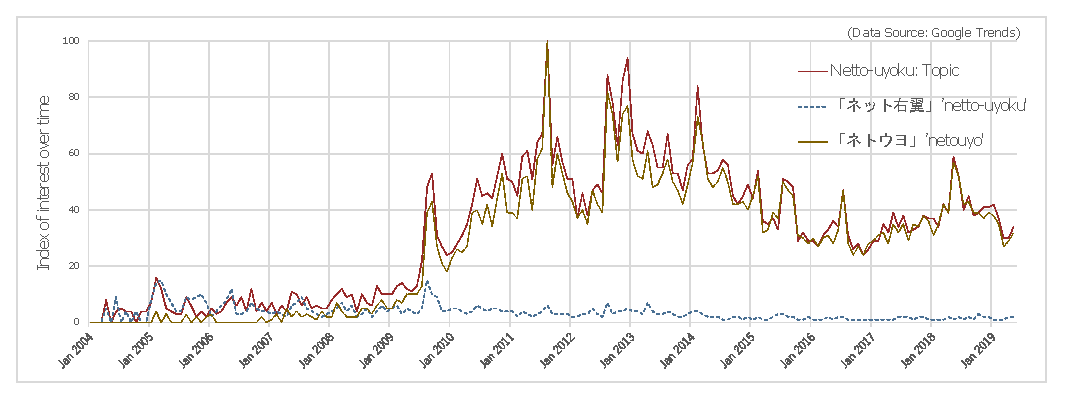
\includegraphics[width=0.95\textwidth,trim=4 4 4 4,clip]{images/nettouyoku2.eps}
\end{figure}

If we look at an estimate of relative interest in the Netto-Uyoku using
Google search queries from the past fifteen years (see \textbf{figure
\ref{fig:nettouyoku}}),\footnote{Google search queries offer a glimpse
  on public awareness and interest in a topic. This graph contrasts the
  term `Netto-Uyoku' as a `Topic' (which includes algorithmically
  collected related keywords) and its breakdown in the literal search
  terms `\emph{netto-uyoku}' 「ネット右」 and `\emph{neto-uyo}'
  「ネトウヨ」. Interest is scaled to the the highest peak of interest
  (100), which is calculated based on the highest amount of queries for
  a term or topic, relative to the total Google search queries at that
  time; it is not an indicator of quantity. For more information on the
  methodology behind Google Trends as well as other relevant graphs, I
  refer to \textbf{\ref{appendix:googletrends}}.} we could assert that
while there was a small rise in public interest after Sasaki's article,
a global awareness of this trend did not appear until the late 2000s,
with peaks coinciding with election lead-ups (such as former Prime
Minister Naoto Kan's resignation and subsequent party election, and the
December 2012 general election). This graph further shows that the more
pejorative `neto-uyo' (「ネトウヨ」) overtakes the more neutral
`netto-uyoku' 「ネット右翼」 in usage from mid-2009 onwards.

\section{Who are the Netto-Uyoku?}\label{who-are-the-netto-uyoku}

It is around this period too that academic interest in the Netto-Uyoku
starts to increase. In one of the earlier English language publications
by those in academia, Morris-Suzuki
(\protect\hyperlink{ref-morris-suzuki_freedom_2013}{2013})\footnote{Tessa
  Morris-Suzuki is professor of Japanese History and frequent
  contributor to \emph{The Asia-Pacific Journal: Japan Focus}. Her
  academic work focuses primarily on the topic of identity and politics
  in Japan.} warns against the dangers of social media as a tool for
populist mobilization, and paradoxical usage of the empty signifier
`freedom of speech'. While not explicitly using the term Netto-Uyoku or
\emph{net-right}, she describes trends of ``violently xenophobic or
racist messages, recycling wartime language and imagery that had long
disappeared from public discourse in Japan'' on the anonymous Internet
forum \emph{2channel} as a trend of ``Internet nationalism''. Based on a
2012 social media white paper showcasing 2channel users to be
predominantly young men, she frames this group as ``lonely, frustrated
\emph{otaku} (an isolated person with obsessive interests), probably
unemployed or in a dead-end job, seeking some sense of identity by
sharing anger and bitterness with nameless others.'' She further hints
that as the social media-scape shifts, so too then finds this
2channel-inspired Netto-Uyoku discourse its way to other platforms. The
image of lonely Netto-Uyoku as \emph{otaku} seeking comfort in
nationalism and group-bonding online is indeed a compelling narrative,
if potentially stereotypical and through such usage of polemic language
at risk of drawing backlash. So how then have other authors addressed
this?

Several years earlier Tsuji
(\protect\hyperlink{ref-tsuji_eng:_2008}{2008}) made a first attempt at
drawing a quantitative view of the Netto-Uyoku demographic. By holding
an online survey with 998 valid participants, Tsuji tried to map
right-wing radicalization and polarization (working on Cass R.
Sunstein's notion of \emph{group polarization}) amongst Internet-users,
and used the following traits to identify Netto-Uyoku:

\begin{enumerate}
\def\labelenumi{\arabic{enumi}.}
\tightlist
\item
  Feelings of antagonism towards China and Korea
\item
  Agreement to the Prime Minister's visit to the Yasukuni
  Shrine\footnote{A Shinto shrine generally commemorating those fallen
    in the service of the Japanese nation from the Meiji period onwards.
    This includes soldiers convicted of war crimes, including Class A
    war criminals during the Second World War, and public visits by
    politicians representing the state has drawn criticism for
    unapologetic, nationalist behavior.}
\item
  Agreement towards the revision of Article 9 of the
  constitution\footnote{Article 9 respectively renounces war (clause 1)
    and deters any legal rights to maintain a national army (clause 2).}
\item
  Agreeing with the display of the national flag and singing the
  national anthem in elementary and middle schools
\item
  Having written on social or political issues on one's website, or
  commented and engaged in discussion on social media online
\end{enumerate}

Out of his sample, thirteen people have had strong agreements to all of
the above (1.3 percent) and, when eased to agreement of three items
including the fifth point, this number increased to thirty-one (3.1
percent). Tsuji concluded that based on these early findings, this group
indeed appears to be dominantly male, frequently participate on
2channel, and has a negative bias towards mass communication. Moreover,
through a multiple regression analysis he concludes that a higher
frequency in usage of 2channel correlates with stronger feelings of
patriotism and exclusivism. Although some concerns could be raised on
the amount of Netto-Uyoku willing to truthfully participate in a
``survey on social awareness'',\footnote{Which is the title of the
  actual survey, \emph{shakai ishiki ni kansuru chōsa}
  「社会意識に関する調査」.} not to mention that the survey itself was
targeting only users between the ages of 20 and 44, this does indeed
suggest tendencies of right-wing polarization on 2channel. He further
expanded upon this research with a 2017 paper, after having again
revisited the survey in 2014. As seen in \textbf{table \ref{tab:tsuji}},
Tsuji broadened his target audience, this time with a reach of 2347
participants aged 20 to 59. For the sake of valid comparison results
limited to the age-groups 20 - 44 in 2014 have been added in brackets
(Tsuji \protect\hyperlink{ref-tsuji_eng._2017}{2017}).

\setlength{\dashlinedash}{0.2pt} \setlength{\dashlinegap}{4.5pt}
\setlength{\arrayrulewidth}{0.2pt}

\begin{table}[!htb]
\footnotesize
\centering
\begin{threeparttable}
\setlength{\tabcolsep}{5pt}
\caption{Ratio of Netto-Uyoku according to 2007 \& 2014 surveys}\label{tab:tsuji}
\begin{tabular}{ l c c c c } 
\toprule
 & \multicolumn{2}{c}{2007 survey} & \multicolumn{2}{c}{2014 survey}\\
 & Ratio (\%) & Total & Ratio (\%) & Total \\ 
 \midrule
 a) Negative Sentiment Towards China and Korea & 36.6 & 362 & 62.7 (60.6) & 1471 (880)\\\cdashline{2-5}
 b) Conservative political orientation & 6.4 & 63 & 11.3 (10.7) & 265 (155)\\ \cdashline{2-5}
 c) Posting or arguing on the Internet & 15.4 & 152 & 12.2 (10.7) & 286 (190)\\ \cdashline{2-5}
 a) Percentage Netto-Uyoku & 1.3 & 13 & 1.8 (1.9) & 43 (28)\\
\bottomrule
\end{tabular}
\caption*{\raggedleft(Source: Tsuji 2017)}
\end{threeparttable}
\end{table}

While Tsuji's conclusions are not drastically different, finding no
significant discrepancies in academic background or income, he confirms
seven years after the initial study that this group of `Netto-Uyoku'
still prefer anonymous communication tools such as 2channel and video
service Niconico over social media as Facebook or the messaging service
LINE. He further suggests that while there is not much of an increase in
users actively attempting to disseminate their political opinions (an
estimated two percent of Internet users), there is at least an increase
in latent Netto-Uyoku behavior when taking in mind the starch rise in
reactionary and xenophobic sentiment\footnote{In particular the idea
  that migrant foreigners will correlate to higher crime rates.} between
2008 and 2014 (Tsuji
\protect\hyperlink{ref-tsuji_eng._2017}{2017}).\footnote{He too argues
  the neo-nationalist ACM demonstrations as a real-life extension of the
  Netto-Uyoku and further refers to them as \emph{Nihon-ban no orutana
  uyoku} 日本版のオルタナ右翼, the Japanese version of the Alt-Right
  (Tsuji \protect\hyperlink{ref-tsuji_eng._2017}{2017}).}

\section{2channel, an imagined
Cyber-village}\label{channel-an-imagined-cyber-village}

2channel, an anonymous message-board developed by Hiroyuki Nishimura (at
the time an exchange student in the United States), was described in an
earlier Wired article as the biggest bulletin board system in the
world---with 2.5 million posts a day (Katayama
\protect\hyperlink{ref-katayama_2-channel_2007}{2007}). The article
paraphrases Daisuke Okabe as saying that 2channel is for its users a
place ``where people can combat the mass media on a grass-roots level,''
evoking through his wording imagery of warfare and suggesting there lies
a subconscious reasoning of the Internet as an ideological Other to
mass-media. Moreover, Katayama quotes 2channel founder Nishimura in
saying, as a reaction to ``more than 50 civil lawsuits in Tokyo alone
and more than \$4 million in settlements and court penalties for libel,
defamation, copyright violations, privacy and personal injury,'' that he
does not have ``any intention of paying up to a country whose laws I
don't respect.'' This again implies an atmosphere of rebelliousness and
one that we could then too associate with the messaging board
itself.\footnote{In another intersection with its English language
  counterpart, it must be noted however that Hiroyuki Nishimura has
  since lost legal ownership of 2channel to the owner of the extreme
  right-wing 4chan spin-off \emph{8chan}, Jim Watkins (Silverman and
  Lytvynenko \protect\hyperlink{ref-silverman_meet_2017}{2017}), and in
  turn himself became owner of 4chan. Furthermore, since Jim Watkins'
  take-over, 2channel now links to 8chan on its front-page. He has since
  gone on to create an intended 2channel rival \emph{2ch.sc}, which has
  attracted some of 2channel's former `population'.}

Kitada (\protect\hyperlink{ref-kitada_eng:_2005}{2005}) argues that this
sense of rebelliousness and scorn towards mainstream media experienced
on 2channel---in other words, a social space of `cynical anti-media
culture'---lies at least in part at the roots of the nationalism
experiences on 2channel. Writing in 2005 about trends of a
`right-leaning tilt amongst youth' (\emph{Wakamono-tachi no ukei-ka},
若者たちの右傾化) shortly before the public adoption of the term
Netto-Uyoku, Kitada observes on 2channel a distinct cynical mode of
communication that relies on harsh bluntness, but one through which its
users develop a sense of intimacy. This mode of communication then
relies on a constant source for critique through which it can sustain
social connections. As Kitada himself states in an English translation
of his 2005 essay, ``From a sociological point of view, 2ch marks a
departure from an instrumental rationality that supports the existing
social order. Instead, it is a social space that produces an extreme
form of connective rationality that supports ongoing communicative
actions and reactions that maintain the community.'' Furthermore, ``what
began as principled attacks on discrepancies between mass media's
ideology and reality have changed into an activity seeking to perpetuate
ironic communication, leading to a paranoid attitude that aggressively
seeks discrepancies between form and content,'' (Itō, Okabe, and Tsuji
\protect\hyperlink{ref-ito_fandom_2012}{2012}, 70--80).\footnote{Kitada
  views this cynical anti-media culture as an extension of an '80s
  consumerist society in which sensibilities of playful irony associated
  with media literacy and intertextuality became vulgarized through
  interaction with popular media. That is to say, a population growing
  up with the medium of TV developed a sense of ironic distance to this
  media, and an insider culture associated with the new mode of
  communication through which youth sought interactivity adopted a
  cynical stance towards ``the discrepancies between mass media systems
  and journalism,'' (Itō, Okabe, and Tsuji
  \protect\hyperlink{ref-ito_fandom_2012}{2012}, 76).}

This channels to certain extent political scientist Anderson's
(\protect\hyperlink{ref-anderson_imagined_2006}{2006}) notion of
\emph{imagined communities}, which Sakamoto
(\protect\hyperlink{ref-sakamoto_koreans_2011}{2011}), Murai
(\protect\hyperlink{ref-murai_net_2012}{2012}) and this author
(\protect\hyperlink{ref-poppe_digitaal_2017}{2017}) have respectively
relied upon in an attempt to explain the sense of kinship shared on an
online medium on which users are clouded in anonymity. Anderson, in his
work on nationalism, draws attention to the transforming role of what he
called \emph{print-capitalism}, the capitalist drive behind
mass-printing in vernacular languages. His idea of nations as `imagined'
communities then implies that the sense of kinship felt between its
members is a social construct based on imagined mutual experiences and
the standardization of language derived from this print capitalism and
its subsequent rise in mass-media. These communities develop a sense of
imagined sameness as well as a clearly defined paradigm of `otherness'.
In that sense, the communities on 2channel (and indeed, on its English
counterpart 4chan) then gain their imagined sense of comradeship through
Kitada's suggested grammar of cynicism; mutual consumption and critique
of mainstream media events and the cynical, harsh language behind it.

This logic has also been covered by media scholar McLuhan and his work
in the 1967 \emph{The Gutenberg Galaxy: The Making of Typographic Man},
expanding upon Harold Innis's \emph{The Bias Of Communication} (1951):
``The effect of the discovery of printing was evident in the savage
religious wars of the sixteenth and seventeenth centuries. Application
of power to communication industries hastened the consolidation of
vernaculars, the rise of nationalism, revolution, and new outbreaks of
savagery in the twentieth century''
(\protect\hyperlink{ref-mcluhan_gutenberg_2011}{2011}, 245). Innis and
in extension McLuhan argued that the invention of print-media
transformed an oral, `time-biased' tribe culture into a literate
`space-biased' culture, changing our mental processes and bringing about
a heightened sense of individual consciousness yet laying the
groundworks for nationalism.\footnote{``The inherent conflict
  {[}\ldots{}{]} is at the centre of print technology itself, which
  isolates the individual yet also creates massive groupings by means of
  vernacular nationalism.'' This inherent conflict refers to the
  conflict of the ``need for self-definition'' with the ``process of
  renunciation of differences''. (McLuhan et al.
  \protect\hyperlink{ref-mcluhan_gutenberg_2011}{2011}, 244)} With his
idea of a `global village', McLuhan hypothesized then that trends
towards electronic media (referring at the time to radio and television)
would again alter society---from a literate culture to a `post-literate'
visual culture, one with different forms of social interaction---that is
to say, one of a collective, homogeneous identity, in which the lack of
a physical body or physical cues creates a different relation to oneself
and one's surroundings (McLuhan et al.
\protect\hyperlink{ref-mcluhan_gutenberg_2011}{2011}, 21--35).

\section{The Action-Conservative Movement
(ACM)}\label{the-action-conservative-movement-acm}

In another early academic work on the Netto-Uyoku, Sakamoto
(\protect\hyperlink{ref-sakamoto_koreans_2011}{2011}) discusses the
Netto-Uyoku (what she abbreviated as \emph{netto-uyo}) as a form of
``Internet nationalism in contemporary Japan.'' She too connects the
Netto-Uyoku to 2channel and Niconico, and adheres to Tsuji's
(\protect\hyperlink{ref-tsuji_eng:_2008}{2008}) earlier classification,
describing the Netto-Uyoku as follows (Sakamoto
\protect\hyperlink{ref-sakamoto_koreans_2011}{2011}, 2--4):

\begin{quote}
Mirroring the post-1990s historical revisionism, netto-uyo exhibit
xenophobia towards immigrants, depict Korea and China negatively, and
uphold revisionist history, justifying and glorifying Japan's wartime
actions. They also support political leaders' official visits to
Yasukuni Shrine, revision of Article 9 of the constitution, and
patriotic education. {[}\ldots{}{]} Netto-uyo's `we the Japanese' does
not even include all ethnic Japanese, as those who do not share their
values (liberals, left-wingers, feminists, supporters of non-Japanese
residents' rights, Korean TV drama fans etc.) are all considered
potential enemies of the nation."
\end{quote}

Sakamoto further calls 2channel\footnote{She abbreviates 2channel as
  2-chan. This should however not be confused with another messaging
  board, Futaba Channel, which is often referred to as 2chan due its URL
  2chan.net.} ``\,`not for the faint of heart', this unmoderated forum
is known to be the main outlet for revisionism and xenophobic
neonationalism of the internet generation''
(\protect\hyperlink{ref-sakamoto_koreans_2011}{2011}, 2). like Kitada,
she concurs that the nationalism occurring on 2channel is not an
extension of preexisting nationalism, saying that ``discourses that
develop on the Internet may exhibit different characteristics from those
that form outside the Internet,'' and further arguing that ``{[}a{]}s
one of the many strands of nationalism that constitute contemporary
Japan's neonationalist landscape {[}\ldots{}{]} 2-chan online
nationalism should not be dismissed as mere chatter,'' (Sakamoto
\protect\hyperlink{ref-sakamoto_koreans_2011}{2011}, 13). Instead, so
she continues, ``{[}a{]}lthough netto-uyo nationalism currently remains
largely within cyberspace, and although cynicism seems to prevail over
modernist commitment to a fixed meaning, the potential for its
politicisation and mobilisation exists''
(\protect\hyperlink{ref-sakamoto_koreans_2011}{2011}, 13).

Although this paper deals primarily with the the potential for
\emph{politization}, illustrations of \emph{mobilization} are abound. In
the light of an increased Fuji Television programming of South Korean TV
series, for example several counter-protests were held in August 2011
drawing an estimate 2,000 to 10,000 participants depending on the source
(Schilling \protect\hyperlink{ref-schilling_japanese_2011}{2011};
Chosun.com \protect\hyperlink{ref-chosun.com_japanese_2011}{2011}; Ilbo
\protect\hyperlink{ref-the_donga_ilbo_japans_2011}{2011}; Itagaki
\protect\hyperlink{ref-itagaki_anatomy_2015}{2015}). Perhaps the most
clear testament to their potential for \emph{mobilization}, though, lies
in the activities of what Yamaguchi
(\protect\hyperlink{ref-yamaguchi_xenophobia_2013}{2013}) translates as
ACM, the Action Conservative Movement (\emph{kōdō suru hoshu undō},
行動する保守運動). As referred to in chapter one, those neo-nationalist
groups are in the literature covered so far intrinsically linked to the
Netto-Uyoku and have held over a thousand documented marches in the
timespan of three years (Nikaido
\protect\hyperlink{ref-nikaido_eng:_2016}{2016}). Higuchi, author of the
2016 \emph{Japan's Ultra-Right}, compares these ACM groups with the rise
of neo-nationalism in Europe and argues that ``{[}w{]}hile Japan's old
radical right is authoritarian, anti-communist, and nationalist, the new
radical right is uniquely characterized by its xenophobia'' (Higuchi and
Castelvetere \protect\hyperlink{ref-higuchi_japans_2016}{2016},
1).\footnote{We see this discrepancy between the neo-nationalism
  associated with the Netto-Uyoku and ACM and `traditional' nationalism,
  by the way, in the criticism by what might be considered the
  `historical' (post-war) far-right movements in Japan (\emph{uyoku
  dantai}, 右翼団体) of those groups as `not being rooted in
  conservative or right-wing ideology' (Yasuda
  \protect\hyperlink{ref-yasuda_eng:_2012}{2012}, 320). The head of the
  \emph{uyoku dantai} `Unification Front Volunteer Army' (\emph{tōitsu
  sensen giyūgun}, 統一戦線義勇軍), for example, criticized the ACM
  group Zaitokukai as not being able to distinct between the Internet
  and reality, acting rashly without experience (Yasuda
  \protect\hyperlink{ref-yasuda_eng:_2012}{2012}, 324--25). Furthermore,
  amongst the representatives of organization formed to counter the
  xenophobia of these groups, \emph{Norikoe netto} (のりこえねっと, a
  contraction of `\emph{Heitosupīchi to reishizumu o norikoeru kokusai
  nettowāku}'
  「ヘイトスピーチとレイシズムを乗り越える国際ネットワーク」, lit.
  ``International network to overcome hate speech and racism'') we find
  not just former Prime Minister of Japan Murayama Tomiichi, as well as
  Yasuda himself, but also founder of the \emph{uyoku dantai} `Issuikai'
  (see footnote \footnoteref{issuikai} on page \pageref{issuikai})
  Suzuki Kunio (Net \protect\hyperlink{ref-net_norikoe_2015}{2015}).
  This group's name is a deliberate reference to the aggressive
  demonstrations held by the Zaitokukai in regards to a Filipino
  schoolgirl, Noriko Calderon, whose parents were deported as illegal
  immigrants.} The ACM's topics of choice, so then writes Meiji Gakuin
University Professor Tom Gill,\footnote{In his paper on the ACM, he
  describes 2channel in a rather negative light as ``an internet site
  which is well known for no-holdsbarred discussion, virulent ad hominem
  attacks and rightist/racist rhetoric'' (Gill
  \protect\hyperlink{ref-gill_nativist_2018}{2018}, 184).} include ``the
lay Buddhist religious movement Soka Gakkai, the Japan Teacher's Union
(\emph{Nikkyōso}), the Buraku Liberation League (\emph{Buraku Kaihō
Dōmei}), the media {[}\ldots{}{]} and sometime the national and local
governments. However, its most striking feature is its hostility to
foreigners in Japan generally, and Koreans in particular,''
(\protect\hyperlink{ref-gill_nativist_2018}{2018}, 176). To reiterate,
the antagonizing of (ethnic) minority groups, foreigners and the media.

While a complete overview of the ACM and a breakdown of their concrete
stances lies beyond the scope of this paper, it is of some essence to
cover the Zaitokukai and its founder Sakurai Makoto, the man who stirred
Fackler (\protect\hyperlink{ref-fackler_new_2010-1}{2010}) to write his
initial \emph{The New York Times} article. Founded in 2006, the
Zaitokukai gained notoriety for its frequent demonstrations throughout
Japan and its aggressive rhetoric mirroring the language used on
2channel. As we might defer from the group's full name, ``The Citizens'
Group Refusing to Tolerate Special Rights for Zainichi Koreans''
(\emph{Zainichi Tokken wo Yurusanai Shimin no Kai}
在日特権を許さない市民の会), their activities are centered dominantly
around the topic of ethnic Koreans residing in Japan\footnote{This paper
  for the sake of brevity refers to the different diaspora with ethnic
  roots in the Korean peninsula and immigration histories tracing back
  to Japan's rule of the peninsula as `ethnic Koreans' (in Japanese,
  usually preceded with the term \emph{zainichi} 在日, literally meaning
  `residing in Japan'). We do not infer that the identity felt amongst
  these groups is homogeneous, and the complexity of the pre-war Korean
  kingdom known as Chosŏn, the post-war North and South Korea, the
  ambiguous legal state of these groups `permanently residing' in Japan
  and the various difficulties of integration these impose goes beyond
  the scope of this paper. When this paper references xenophobia as an
  ideological element of Netto-Uyoku or ACM, this includes the logic of
  viewing those `ethnic Koreans' as non-Japanese and not belonging.},
with protests often held in neighborhoods with large concentrations of
ethnic Koreans. Nevertheless, they often engage in attacks on media due
to a supposedly biased programming towards Korean pop-culture and
`concealment' the truth (e.g.~crimes supposedly committed by those
groups), and have engaged in reactionary protests against left-wing
counter-protests (on topics such as nuclear energy).\footnote{See for
  example the ``Demonstration march for not extinguishing the fire of
  nuclear plants'' (\emph{genpatsu no hi o kesasenai demo kōshin}
  「原発の火を消させないデモ行進」), a counter counter-protest in
  Shibuya on April 17, 2011, held in the belief that anti-Japanese
  left-wingers purposefully intend to weaken Japan from the inside by
  limiting its energy sources (Sakurai
  \protect\hyperlink{ref-sakurai__2011}{2011}).}

Freelance journalist and author of ``The Internet and Patriotism''
(``\emph{Netto to Aikoku}'', 『ネットと愛国』) Yasuda
(\protect\hyperlink{ref-yasuda_eng:_2012}{2012}) extensively covered the
Zaitokukai; conducting interviews with its members and
supporters\footnote{In 2017, the Zaitokukai's main page claimed a
  membership of 16399 people, of which 14079 (85,85\%) were male (Poppe
  \protect\hyperlink{ref-poppe_digitaal_2017}{2017}, 24--25). As of
  writing, the Zaitokukai web-page referred to is no longer online.} as
well as those who've known the Zaitokukai's founder as a child. Yasuda
found that, in spite of rhetoric inciting violence (at times including
the actual usage of violence)\footnote{For which Sakurai and three other
  members of the Zaitokukai were arrested. This article too reached the
  print edition of \emph{The New York Times} courtesy of Martin Fackler
  (Fackler \protect\hyperlink{ref-fackler_japanese_2013}{2013}).} and
racial pejoratives, its members are generally speaking `normal'
citizens.\footnote{Although going to some extents to include the social
  or economical exclusion felt by those supporters.} Higuchi
(\protect\hyperlink{ref-higuchi_japans_2014}{2014}) drives this point
further, stating they are `normal' in the sense that based on his
surveys, they do not even stand out due to economic malaise or for being
on the fringes of society. Furthermore, a common trait of these groups
is, unlike the mostly male-dominated post-war nationalist groups
collectively known as \emph{uyoku dantai} the inclusion of women; with
various ACM groups solely built around the female identity.\footnote{Gill
  sums several of these up, such as the ``\emph{Nippon Josei no Kai
  Soyokaze} (Japan Women's Association Breeze), its offshoot
  \emph{Aikoku Josei no Tsudoi Hanadokei} (Patriotic Women's Gathering
  Flower Clock), \emph{Zenkoku Hoshu Josei Rengō} (National Conservative
  Women's Alliance) and \emph{Nadeshiko Akushon} (Japanese Women for
  Justice and Peace)'' (Gill
  \protect\hyperlink{ref-gill_nativist_2018}{2018}, 176).} Yamaguchi
(\protect\hyperlink{ref-yamaguchi_xenophobia_2013}{2013}) argued earlier
that ACM groups such as the Zaitokukai pay strong attention to the
normative aspect of being `normal members of society'. This inclusive
role is then purposely done, to quote Yamaguchi, ``to enhance the
`ordinariness' of the ACM. Women are encouraged to deliver speeches,
walk in front of the group, and wear the kimono not only as the epitome
of Japanese women's tradition but for visual impact''
(\protect\hyperlink{ref-yamaguchi_xenophobia_2013}{2013}, 104).

Morris-Suzuki
(\protect\hyperlink{ref-morris-suzuki_freedom_2013}{2013}), like Yasuda,
Higachi and Yamaguchi, noted the Zaitokukai's active use of social media
for propagating ideology, hinting at a radicalizing effect by claiming
that such media usage is how the Zaitokukai ``recruit the
young.''\footnote{Their usage of hate speech then, while through various
  interpretations of the Penal Code illegal, so argues Morris-Suzuki,
  goes unpunished ``because such laws could limit freedom of speech.''}
Indeed, its core members are savvy Internet-users using Twitter,
Niconico and Youtube to spread videos of their protests,\footnote{In an
  interview, one of its members points out that the protests serve as
  vehicle to broadcast online
  (\protect\hyperlink{ref-yamaguchi_xenophobia_2013}{2013}, 108).
  Niconico has since, under influence of the 2016 anti-discrimination
  law, removed the Zaitokukai's account (Furuya
  \protect\hyperlink{ref-furuya_can_2016}{2016}\protect\hyperlink{ref-furuya_can_2016}{b}).
  Youtube and Twitter have taken similar actions.} and this author
(\protect\hyperlink{ref-poppe_digitaal_2017}{2017}) further pointed out
the stylistic resemblance of the Zaitokukai's homepage to 2channel, as
well as the usage of sub-culture elements as cartoon characters to drive
their arguments.\footnote{Moreover in a mixed-methods content analysis
  of a corpus of approximately 3200 Twitter messages (including
  retweets) of the Zaitokukai's founder, this author
  (\protect\hyperlink{ref-poppe_digitaal_2017}{2017}) found the topics
  to be dominantly centered around antagonizing South Korea and
  left-wing politics (using the pejorative term \emph{payoku} パヨク,
  `leftists').} As Yamaguchi and Gill argue, they draw on a social
anxiety that began in the early 2000s with the public acknowledgment of
North Korean kidnappings of Japanese civilians, as well as protests with
anti-Japanese sentiment held throughout East-Asia in 2005, and
economical stagnation in the face of China and South Korea's rapid
growth. It is nevertheless not just an outsider group's radicalizing
usage of media, that is of note. Rather, it could be argued that it is
within this right-leaning cynical Internet discourse itself that the
Zaitokukai arose.\footnote{Summarized as, ``the Internet too was a
  catalyst for encouraging Sakurai's activities.'' (\emph{Netto wa
  Sakurai jishin no hiyaku o mo unagasu kikkake tomo natta},
  「ネットは桜井自身の飛躍をも促すきっかけともなった」), Yasuda too
  suggests that it was within the discourse of the Internet that
  Zaitokukai founder Sakurai Makoto was able to rise (Yasuda
  \protect\hyperlink{ref-yasuda_eng:_2012}{2012}, 45).} Its founder,
going by the pen name Makoto Sakurai,\footnote{In the wake of the arrest
  of several Zaitokukai-members, News
  (\protect\hyperlink{ref-nikkei_news__2013}{2013}) published an article
  revealing his birth name to be Takada Makoto (高田誠). Due to the wide
  spread usage of his pen name, I will continue to refer to him as
  Sakurai Makoto.} started his anti-Korean activities (\emph{kenkan
katsudō}, 嫌韓活動) during the 2002 FIFA world championship organized in
South Korea, claiming in an interview with the conservative right-wing
newspaper \emph{Sankei Shimbun}
(\protect\hyperlink{ref-sankei_news__2016}{2016})\footnote{One of the
  few mainstream outlets covering his political ambitions during the
  2016 Tokyo gubernatorial elections.} that despite immense support from
Japan, Sakurai noted an anti-Japanese presence on the Internet, with
such slogans as ``Lose, Japan!'' (\emph{nihon makero} 「日本負けろ」)
making its way on anonymous messaging boards.

\begin{figure}[!htb]
 \centering
 \begin{subfigure}[b]{0.30\textwidth}
  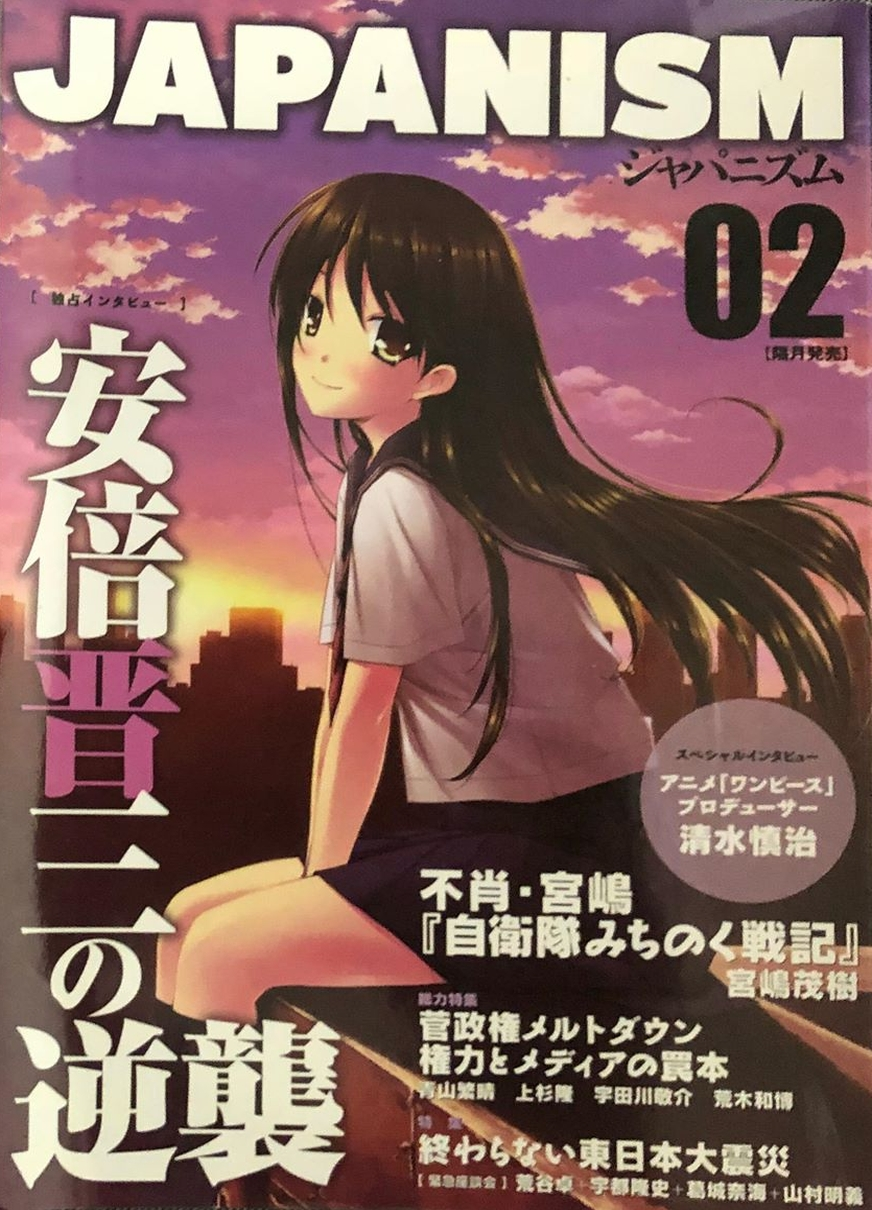
\includegraphics[width=\textwidth]{images/japanism1.jpg}
  \caption{Volume 2, June 2011. "Exclusive interview: Abe Shinzō's counterattack"}
  \label{fig:twitter1}
 \end{subfigure}
  \begin{subfigure}[b]{0.30\textwidth}
  
\includegraphics[width=\textwidth]{images/japanism4.jpg}
  \caption{Volume 15, October 2013. "Major feature: That's enough, South Korea!"}
  \label{fig:twitter2}
 \end{subfigure}
 \caption{Covers of Magazine 'Japanism'}\label{fig:twitter}
\end{figure}

Before going on to start the Zaitokukai in 2006, run for Tokyo Governor
in 2016 and start a political party in 2017 (the Japan First Party,
\emph{Nippon daiichi tō} 日本第一党), much of his early `career' as a
self-proclaimed political activist happened online and in interaction
with similar forms of neo-nationalism occurring on the South Korean
Internet.\footnote{Going in discussion with South Koreans on forums
  backed with automatic translation software (\emph{hon'yaku keijiban}
  翻訳掲示板), including that of Korean Internet portal NAVER. Murai
  references the VANK (Voluntary Agency Network of Korea), who took part
  in cyber-attacks on 2channel and in turn spread similar aggressive
  rhetoric on the Internet. As Murai states, ``Ironically, such
  conflicts of radical nationalism have given credibility to Net Uyoku's
  radical ideology'' (Murai
  \protect\hyperlink{ref-murai_net_2012}{2012}, 374).} It is only
through his continuous online activities\footnote{Including one website
  ``The Strange Country, South Korea'' (fushigi no kuni no kankoku
  「不思議の国の韓国」, a pun on ``Alice in Wonderland'', \emph{fushigi
  no kuni no arisu} 『不思議の国のアリス』), a forum ``live discussions
  on Korea'' (kankoku nama tōron 「韓国生討論」) and a blog under his
  longtime user-name \emph{Doronpa01}.} that Sakurai received an initial
invitation to star as guest member on the Nippon TV (日本テレビ)
variety-show `Generation Jungle' (\emph{jenejan}, 「ジェネジャン」),
became frequent contributor to the bi-monthly conservative magazine
Japanism (\emph{`japanizumu'}, 「ジャパニズム」)\footnote{Published by
  \emph{Seirindō}, the publishing house behind the influential
  underground manga anthology Garo (ガロ) and more recently, several
  other of Sakurai's writings, including the 2014 ``Great Korean Hate
  Era'' (``\emph{dai kenkan jidai}'', 『大嫌韓時代』 and the 2016
  ``Great Korean Hate Dictionary'' (``\emph{dai kenkan nikki}'',
  『大嫌韓日記』). The magazine, as well as the publishing house
  Seirindō, have gone through different editors-in-chief, with a gradual
  shift towards political topics.} and eventually in 2006 started the
Zaitokukai.\footnote{In October 2014 Sakurai participated in a recorded
  debate with former mayor of Osaka, Hashimoto Tōru. This ended several
  minutes after both parties engaged in verbal insults (2021 summer
  \protect\hyperlink{ref-2021_summer_vs_2014}{2014}). Sakurai stepped
  down as Zaitokukai leader shortly after.} As we can further defer from
\textbf{figure \ref{fig:murai-ratio}}, that latter magazine, which
started its print in April 2011 shortly after the March 11 Earthquake,
is a suitable example of Azuma's suggestion of subcultured nationalism,
wherein content that is highly ideological is juxtaposed with elements
of \emph{otaku} subculture.

\section{From 2channel \&
Niconico\ldots{}}\label{from-2channel-niconico}

Moving away from views of neo-nationalism on the Internet decidedly as
an expression of social anxiety, Sakamoto
(\protect\hyperlink{ref-sakamoto_koreans_2011}{2011}) too shifts her
point of focus on the discursive practices of building identity and
nationalism online. For that, she conducts a content analysis of one
thread on 2channel, involving the discussion of a YouTube clip on
Tsushima Island,\footnote{An island located in between Japan and the
  Korean Peninsula. Due its location, it is one element in the
  territorial despites (and the larger nationalist conflicts) between
  South Korea and Japan.} which gained 7000 reactions over a time span
of four days. According to her analysis, the majority of comments
deferred from the original topic at hand and serve simply to reinforce a
negative portrayal of Koreans as the cultural Other; that is to say, an
empty signifier symbolizing that what is ``\,`inferior', `dirty',
`shameless', `primitive', `violent', and `irrational'\,'', which then in
the process implies the Japanese participants on these threats to be the
opposite (Sakamoto \protect\hyperlink{ref-sakamoto_koreans_2011}{2011},
7).

\begin{quote}
\begin{quote}
``Collectively, the 7,000 postings produced and reinforced the negative
image of Korea and Koreans far beyond the Tsushima issue. Forum
participants brought up a multitude of Korea related issues which had
nothing to do with Korean tourists on Tsushima: the `special tax and
welfare privileges' that zainichi Koreans allegedly enjoy, the `illegal
occupation' of Takeshima Island', kimchi with parasite eggs, or crimes
by Koreans in Japan and overseas. Links were made to a TV news item
about a Japanese boy who was attacked in Korea, snapshots of
anti-Japanese artwork by Korean school children, a Youtube clip on a
rape by a zainichi Korean, 2-chan threads on zainichi pension
entitlement and welfare benefits, shocking images of anti-Japanese
demonstrators slaughtering pheasants (Japan's national bird) in front of
the Japanese Embassy, and many more. These and other unrelated events
and images are linked together under the unifying but empty sign of the
`Koreans','' (Sakamoto
\protect\hyperlink{ref-sakamoto_koreans_2011}{2011}, 5).
\end{quote}
\end{quote}

Sakamoto discusses the often decontextualized, historically revisionist
(or rather, ahistoric) usage of events and imagery in this thread in the
context of French sociologist Baudrillard's theorization of simulacra,
simulation, the hyper-real and the construction of reality. Although
this is but one interpretation of highly dense theory, simulation for
Baudrillard has in consumerist society come to no longer
\emph{represent} or \emph{copy} reality, but is through discursive
processes a \emph{real} that is not grounded in reality; or to put it in
Baudrillard's exact words ``a real without origin or reality''
(Baudrillard \protect\hyperlink{ref-baudrillard_simulacra_1994}{1994},
1). For Baudrillard, culture and media replace our understanding of an
`\emph{actual}' reality and meaning with simulations and simulacra; with
the \emph{idea} of reality. (Sakamoto
\protect\hyperlink{ref-sakamoto_koreans_2011}{2011}, 9) argues as
follows:

\begin{quote}
Baudrillard's point was that simulation proliferated as a result of the
new media like TV, but the Internet as a participatory medium carried
this trend even further. 2-chan users are not just passive consumers of
such signs provided by the mass media but are producing, performing, and
exchanging referentless, decontexualised signs to generate a sense of
belonging to a cyber community and a fantasy `Japan'.
\end{quote}

The notion of a \emph{fantasy} Japan both consumed and produced by
Netto-Uyoku is not unlike cultural critic Azuma Hiroki's
(\protect\hyperlink{ref-azuma_otaku:_2001}{2001}) critique of otaku.
Azuma argues that although the imagery \emph{otaku} consumed and produce
stems from an imitation of American pop-culture (in particular Disney
animation), attempts are made to draw connections to pre-war traditions
(in particular the Edo-period of 1603-1868) and portray this subculture
and the media they consume as uniquely Japanese. Moreover, traditional
Japanese motifs in wholly unrelated genres such as science fiction serve
to reinforce an imagined \emph{fantasy} or \emph{pseudo}-Japan
(\emph{giji nihon}, 疑似日本). This pseudo-Japan, argues Azuma, stems
from a psychological need for self reenforcement due to the loss of
traditional identity after the Second World War, and again due to
on-going contradictions in society reaching its peak after the narrative
of economical growth collapsed in the '90s (Azuma
\protect\hyperlink{ref-azuma_otaku:_2001}{2001}, ch.1). Moreover, Azuma
puts right-wing ideologies in Japan in direct correlation to this
\emph{otaku} subculture, arguing that ``it can be said that Japan's
right-wing discourse has generally survived through processes of
becoming subcultured, falsified and \emph{otaku}-ized.'' (Azuma
\protect\hyperlink{ref-azuma__2007}{2007}, 23).\footnote{``\emph{Nihon
  no uyoku-teki gensetsu wa ippan ni sabukaruchā-ka shi feiku-ka shi
  otaku-ka suru koto de ikinokotte kitatomo ieru.}'',
  「日本の右翼的言説は一般にサブカルチャー化しフェイク化しオタク化することで生き残ってきたとも言える。」
  (Azuma \protect\hyperlink{ref-azuma__2007}{2007}, 23).} One could then
read Baudrillard's notion of simulations and simulacra in this argument,
stating that those Japanese motifs in Japanese sub-cultural media
associated with \emph{otaku} are exactly such examples of a referentless
\emph{real}---a mediated hyper-reality that precedes actual reality.

\begin{figure}[!htb]
 \centering
 \begin{subfigure}[b]{0.75\textwidth}
  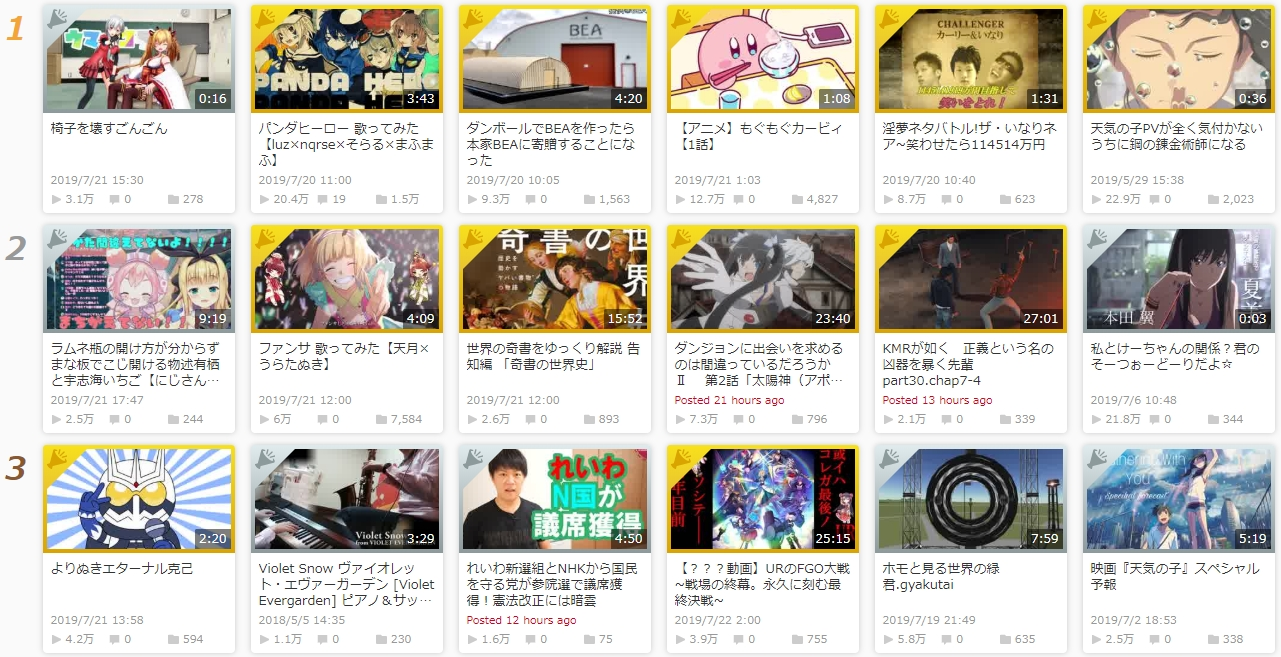
\includegraphics[width=\textwidth]{images/2channel/niconico.jpg}
  \caption*{(Screenshot by author. Source: nicovideo.jp)}
  \label{fig:nicotop}
 \end{subfigure}
 \caption{Screenshot of Niconico's top ranking category (July 23, 2019)}\label{fig:aa}
\end{figure}

If there is one platform illustrating Azuma's and Sakamoto's
interpretation of Baudrillard, it would be Niconico (\emph{nikoniko}
ニコニコ). Founded in 2006 as a video sharing service similar to YouTube
and as of July 2019 the \nth{10} most visited website in
Japan,\footnote{Based on Alexa ranking. For a full list of the top fifty
  most popular pages, see \textbf{table \ref{tab:50mostpopjp}}. Alexa
  statistics further reveal that half of 2channel's audience overlaps
  with that of Niconico (Alexa
  \protect\hyperlink{ref-alexa_alexa_2019}{2019}).} Niconico caters (as
illustrated in \textbf{figure \ref{fig:nicotop}}) primarily to
sub-cultural groups with a focus on Japanese animation or video-games
(or what has arguably since transcended to pop-culture status). Niconico
nevertheless contains a category with topics related to society,
politics and news, and is since used for broadcasting political
discussions and information on elections. Furthermore, its founding
coincides with the start of ACM groups as Zaitokukai and its
functionality and overlap with 2channel (Hiroyuki Nishimura himself
served as CEO for the company behind Niconico, Dwango), as referred to
in the earlier section, was exploited upon by those groups. Niconico has
since expanded as web-portal with a dedicated online news service,
Niconico News (ニコニコニュース),\footnote{Tsuji
  (\protect\hyperlink{ref-tsuji_eng._2017}{2017}) asserts that
  Netto-Uyoku are significantly more likely to read Niconico News, MSN
  Sankei News and jiji.com as their counterparts
  (\protect\hyperlink{ref-tsuji_eng._2017}{2017}, 217)} a comics service
and online dictionary.

While functionally similar to what YouTube offers, Niconico
distinguishes itself further through the ability to place time-synced,
horizontally scrolling comments on top of the video playing. Niconico is
therefore not just reliant on user generated content, the content itself
is actively transformed by those same users. While this brings about an
imagined sense of community as envisioned by Kitada
(\protect\hyperlink{ref-kitada_eng:_2005}{2005}), it could be argued
that not unlike a laugh track on prime-time sitcoms indicating comical
beats, such methods creates a standardized, homogeneous reaction to
particular beats in the video. In a 2013 \emph{Japan Times} article
Journalist Mie (\protect\hyperlink{ref-mie_xenophobia_2013}{2013})
paraphrases DPJ's then-Secretary General Azumi Jun in criticizing Abe's
proposal to campaign on Nico Nico exactly because ``Net uyoku often
alter such videos by directly overlaying their comments on
them.''\footnote{A 2013 \emph{Tokyo Shimbun} article claimed that Hirai
  Takuya, current minister in charge of information technology policy,
  minister of State for ``Cool Japan'' and accredited developer of the
  LDP-themed iPhone game Abepyon (あべぴょん), wrote jeering comments
  aimed at opposition leaders using this function while watching a live
  broadcast of a political debate on Niconico (Tokyo Shimbun
  \protect\hyperlink{ref-tokyo_shimbun_tokyo_2013}{2013}), which has
  since become a running joke.}

\begin{figure}[!htb]
 \centering
  \caption{\label{fig:murai-ratio} Breakdown of videos in (Niconico) "Politics" category.}
 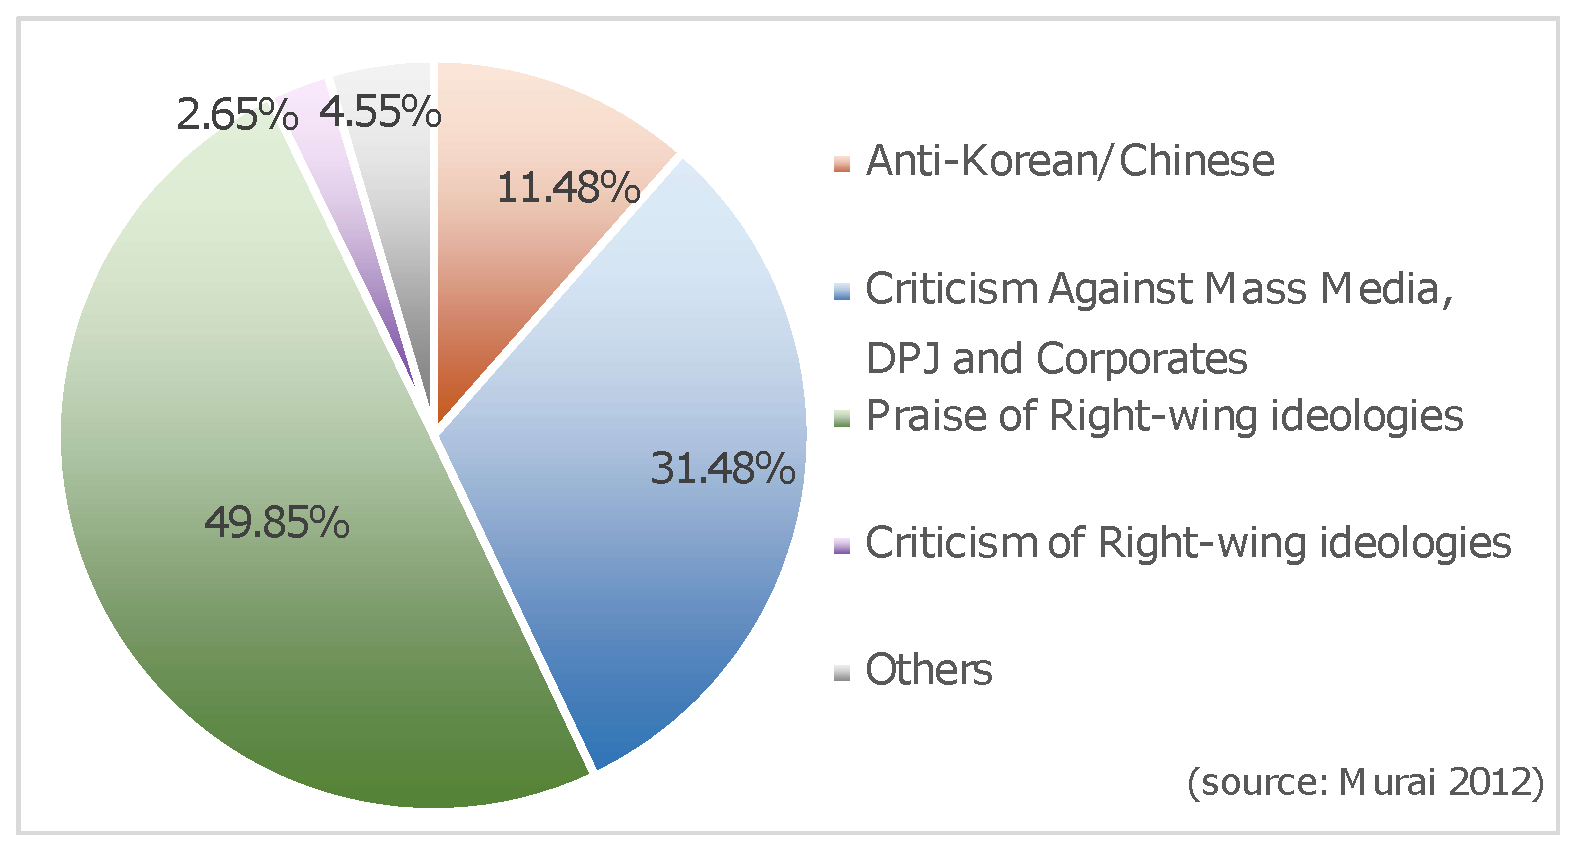
\includegraphics[width=0.65\textwidth,trim=4 4 4 4,clip]{images/murai-ratio2.eps}
\end{figure}

Murai (\protect\hyperlink{ref-murai_net_2012}{2012}) uses Tsuji's above
classification to identify videos containing Netto-Uyoku ideologies,
finding 92.8\% (3712/4000) of the top ranking videos in the `Politics'
category to be as such (see \textbf{figure \ref{fig:murai-ratio}} for a
breakdown per topic). In his content analysis, he describes these videos
as deviant from the ``recreational atmosphere of the other categories'',
containing political messages negative towards East Asian nations, the
Democratic Party of Japan (DPJ) and the ``anti-Japanese'' mass media. He
goes on to claim ``these conservative videos are usually filled with
sympathetic comments by anonymous viewers'' and that ``videos to condemn
imagined enemies are filled with harsh language, while scenes of
`patriotic' activities are praised as heroic.'' He fears that due to the
mass quantity of such videos in the `Politics' section, those political
views will be perceived as the standard and have a radicalizing effect
on a demography of mostly teens and those in their twenties (Murai
\protect\hyperlink{ref-murai_net_2012}{2012}, 369--71).

\#\#\ldots{}Into the Twitter-sphere

Whereas 2channel and Niconico, despite undeniable high in usage, still
have an image of subculture, Twitter has rooted itself firmly amongst
Japanese Internet users, and is as of 2019 the \nth{6} most visited
website in Japan, proceeding less anonymous social media as Facebook.
Furthermore, as Schäfer, Evert, and Heinrich
(\protect\hyperlink{ref-schafer_japans_2017}{2017}) points out, in 2013
the Japanese language became the second most used language on Twitter.
Moreover, according to a 2019 Bloomberg article, Japan became Twitter'
second-largest market, reaching in 2016 a milestone of one-third of
Japan's population logging onto the site at least once every month (Wang
\protect\hyperlink{ref-wang_how_2019}{2019}). Nevertheless this article
refers to ``hateful tweets that have targeted minority groups'' and
indeed, literature on the Netto-Uyoku has covered seepage of 2channel
and its rhetoric onto Twitter.

In 2015, Kanagawa University lecturer Taka Fumiaki held two quantitative
text analyses of respectively a corpus of data containing Twitter
messages pertaining to (ethnic) Koreans and one to China. Taka claims
that since the 2011 earthquake, ethnic Koreans and those with out a
Japanese passport residing in Japan have seen an increase in hate, libel
and false rumors (\emph{dema} デマ). Between the period of November 5,
2012 and February 16, 2013, Taka collected Korean-related tweets with a
final corpus of 109,589 tweets,\footnote{Which due the limitations of
  collecting data on Twitter cannot be claimed to be exhaustive.}
whereof 48,934 were retweets. Through a frequency analysis of the
contents of the tweets (which he further codified into topics such as
politics, historical problems, racism, 2channel, the call for
dispersion, etc), Taka revealed that terms associated with
socio-political tensions or hate-speech far outweigh references to
Korean pop-culture. Finally, through a sentiment analysis, he found the
majority of those messages (70\%) to be negative. Moreover, they are
dispersed by a small group of users intending these messages to be
further shared. Moreover, he examined a distrust of mass media, reliance
or links to 2channel and 2channel curated aggregation sites
(\emph{matome}-blogs), a belief in a ``hidden truth''
(\emph{``\,`Shinjitsu' ga kakusa rete iru to iu shin'nen''}, 「``真実''
が隠されているという信念」) and critique of anything self-identified as
anti-Japanese (Taka
\protect\hyperlink{ref-taka_twitter_2015-1}{2015}\protect\hyperlink{ref-taka_twitter_2015-1}{b}).
His analysis of the corpus pertaining to China (a final corpus of 67,884
Tweets collected between September 19, 2012 and November 5, 2012,
whereof 25,139 were Retweets) revealed the same trends, with beliefs in
truths hidden by mass media, negative sentiment that outweighs the one
seen in the Korean-related corpus; most likely the effects of South
Korea's soft-power (Taka
\protect\hyperlink{ref-taka_twitter_2015}{2015}\protect\hyperlink{ref-taka_twitter_2015}{a}).

Aichi Prefectural University lecturer Brett Hack follows up on Azuma's
notion of a pseudo-Japan and the subcultured status of nationalist by
referring to the \emph{otaku} subculture elements amongst the
Netto-Uyoku, describing the Netto-Uyoku as ``an online subculture
gravitating around a core of nationalist and historical revisionist
beliefs inflected with intense xenophobia'' (Hack
\protect\hyperlink{ref-hack_subculture_2016}{2016}, 34). On the topic of
Twitter, Hack refers to its presence in the form of the `Japanese flag
group' (`\emph{hi no maru kurasuta}', 日の丸クラスタ), users with
Netto-Uyoku tendencies who have the Japanese flag in their profile
picture, preferably in combination with elements of Japanese animation,
militaristic imagery or both.

\begin{figure}[!htb]
 \centering
 \begin{subfigure}[b]{0.40\textwidth}
  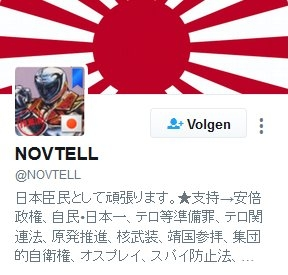
\includegraphics[width=\textwidth]{images/twitter1.jpg}
  \caption{"I will do my best as a Japanese subject. Support: Abe administration, LDP, Japan First Party, anti-terrorism law, terror related laws, promotion of nuclear power, nuclear arms, Yasukuni Shrine visits, right to collective self-defense, Osprey, anti-spy law" (Source: Twitter)}
  \label{fig:twitter1}
 \end{subfigure}
  \begin{subfigure}[b]{0.40\textwidth}
  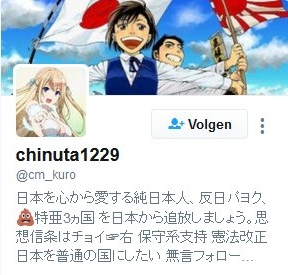
\includegraphics[width=\textwidth]{images/twitter2.jpg}
  \caption{"I'm a pure Japanese person who loves Japan from the bottom of my heart. Let's banish the anti-Japanese leftists and three Tokutei Asia countries from Japan. My thoughts and beliefs are somewhat right. I support conservatives and the constitutional amendment; I want to make Japan a normal country." (Source: Twitter)}
  \label{fig:twitter2}
 \end{subfigure}
 \caption{Examples of Netto-Uyoku Twitter-accounts}\label{fig:twitter}
\end{figure}

\textbf{figure \ref{fig:murai-ratio}} illustrates this. The rhetoric
used in the description of both user pages further fits Tsuji
(\protect\hyperlink{ref-tsuji_eng:_2008}{2008})`s classification of
Netto-Uyoku to a tee. \textbf{Figure \ref{fig:twitter1}} usage of
\emph{Japanese subject} (\emph{Nihon shinmin} 日本臣民) brings to mind a
pre-war Japan with Japanese citizens as the subject of the Japanese
Emperor. This user further expresses his support both for the LDP and
the Japan First Party founded by Zaitokukai's founder Sakurai Makoto.
The laws in question\footnote{The anti-terror laws refer to preemptive
  measures controversial for expanding police powers and threatening
  civil rights (Harding
  \protect\hyperlink{ref-harding_japan_2017}{2017}). The right to
  collective self-defense refers to article 9 of the Japanese
  constitution.} as well as the call for nuclear power, the visits to
Yasukuni Shrine and the military aircraft Osprey\footnote{A military
  aircraft intended for deployment by the Japanese Self-Defense Forces.}
are highly controversial topics and seem to be included more as a
reactionary, polemic statement. \textbf{Figure \ref{fig:twitter2}} uses
the normative 'Normal Japanese' construct; this users support for
constitutional amendment, patriotic feelings and negative feelings
towards the left-wing (\emph{payoku}, パヨク)\footnote{A derogative term
  signifying left-wing ideologues, which this paper loosely translates
  as `leftists'.} and three `Tokutei' countries (\emph{Tokua san-kakoku}
特亜三ヵ国)\footnote{Tokutei Asia (Specific Asia) is a pejorative for
  South Korea, North Korea and China as countries considered to have
  anti-Japanese sentiment.} is normal, perhaps leaning a tad on the
right (\emph{choi migi}, チョイ右).

In their quantitative approach to Netto-Uyoku's usage of bots to spread
political propaganda during the 2014 General Election, Schäfer, Evert,
and Heinrich (\protect\hyperlink{ref-schafer_japans_2017}{2017}) asserts
the importance of the Internet and social media in the outcome of
Japan's General Election of 2014, arguing that ``it was not only with
the support of ``assertive conservative organizations'' such as
\emph{Nippon Kaigi} but also with the help of netto uyo, manipulating a
huge cyber army of bots on Twitter pushing a similar nationalist agenda,
that Abe was successful in the last election,''
(\protect\hyperlink{ref-schafer_japans_2017}{2017}, 4). Furthermore,
Schäfer, building on Kitada
(\protect\hyperlink{ref-kitada__2008}{2008})'s aforementioned
theorization of cynicism as trait of 2channel and its associated
Netto-Uyoku, argues that ``political bots play an important role in this
cynical online strategy of Japanese Internet right-wingers,''
(\protect\hyperlink{ref-schafer_japans_2017}{2017}, 6).

Bots, Schäfer's study, refer to ``computer-generated programs that post,
tweet, or message of their own accord'' (Schäfer, Evert, and Heinrich
(\protect\hyperlink{ref-schafer_japans_2017}{2017}), p.10) in Schäfer,
Evert, and Heinrich (\protect\hyperlink{ref-schafer_japans_2017}{2017})
collected, in a timespan of weeks before- until the day after the
election, a sample of 542,584 tweets related to the election. Using

\section{Politics}\label{politics}

She recalls an incident in January 2001, when shortly before the planned
public broadcast of an NHK documentary on wartime acts of violence
against women by the Japan military, the national broadcast service NHK
was forced to cut parts including testimony and preliminary findings.
The reason for this, as turns out later, was an implied censorship and
political interference by Abe Shinzo, unsupportive of the biased nature
of the show. As the media-scape shifted, however, so too did Abe Shinzo
and a number of Japanese politicians including Hashimoto Toru take ``to
social media with great enthusiasm.'' In particular, she recalls an
incident in which Abe's secretary mobilized Abe's friends and followers
on his Facebook page (at the time counting at respectively 4,800 and
230,000) for an online attack, again, on the NHK (including a \emph{fake
news} story of one panel member on the show). Rather than condemning
this, and contradictory to his public statement of ``Japan's diplomacy
must always be rooted in democracy'' in 2012," Abe instead perpetuates
this attack by responding to that public message on his Facebook with
another \emph{ad hominem} attack.\footnote{She ends with a cautious
  warning that, reminiscent of Karl Popper's \emph{paradox of
  tolerance}, ``democracy is left impoverished when freedom of hate
  speech is protected more zealously than freedom of reasoned political
  debate'' Morris-Suzuki
  (\protect\hyperlink{ref-morris-suzuki_freedom_2013}{2013}).}

\begin{quote}
Tomorrow, the elections deciding the future of Japan finally begin. The
emerging China will not hide their territorial ambitions from Japan. The
illegal landing of the leaders of Korea and Russia on the northern
territories and Takeshima. Moreover, North Korea's missile launch. How
should we respond to such a crisis? Will we sit on our hands with
stopgap measures? Or will we build a new diplomatic history? If Japan
changes even just a little through this Internet call, it will be the
beginning of a new history. {[}\ldots{}{]} And thus, on the last day the
finale will be held by Mr.~Taro Aso as a street address in Akihabara
(electricity street exit) from 19:00 at night. It may be cold, but if we
can fill Akihabara Ekimae with determined people, Japan will without a
doubt change. Why don't we let those in the mass media saying, ``On the
\emph{internet}\ldots{} (italics added by the author to imply derogatory
intent)'' recognize the power of grass roots? Be sure to participate.
Let's change Japan from Akihabara!" (Abe
\protect\hyperlink{ref-abe_1_2012}{2012}) (English translation by the
author)
\end{quote}

https://lite-ra.com/2019/07/post-4813.html

Japanese lawyer Tomomi Inada, who has served under Abe Shinzō as
Minister of Defense and Minister in charge of the Cool Japan Strategy,
is another member of the Nippon Kaigi. She has made controversial
statements regarding stock elements of Japanese nationalism, such as
denial in part of the Nanking Massacre and the Comfort Women system,
stating there is no need to continuing expression of remorse towards
other Asian countries.

(zaitokukai donations?)

\section{Conclusion}\label{conclusion}

As Gill points out, the actions associated with the ACM and in
particular the Zaitokukai appear to be in decline. Since 2014 the amount
of ACM demonstrations has steadily decreased, Sakurai's debut in
politics has seen little success (albeit finishing fifth out of 21
candidates during the Tokyo gubernatorial elections) and the Zaitokukai
and its associated members' various online accounts have under pressure
of anti-hate speech legislation since been removed (Gill
\protect\hyperlink{ref-gill_nativist_2018}{2018}, 189--90). Furthermore,
since Google (both in Japan and worldwide the most used search-engine
and visited website) implemented its knowledge Panels, which draws its
content from a variety of sources including Wikipedia, a Google search
for Zaitokukai reveals decidedly negative content, further impacting
public perception of this group. As seen in \textbf{figure
\ref{fig:googlezaitokukai}}, both images contain a snapshot with imagery
of Adolf Hitler, and the English version in particular refers to
political extremism and terrorism.\footnote{This framing is not a
  deliberate choice by anyone related to Google and instead relies on
  user-generated content. This works however as a double-edged sword, as
  an unrelated Google search for Journalist Jake Adelstein revealed a
  knowledge panel containing an as of July 29, 2019 not-yet-removed
  Wikipedia edit stating ``Jake Adelstein is an American journalist,
  crime writer, anti-Japanese bigot, and blogger who has spent most of
  his career in Japan.''}

\begin{figure}[!htb]
 \centering
 \begin{subfigure}[b]{0.40\textwidth}
  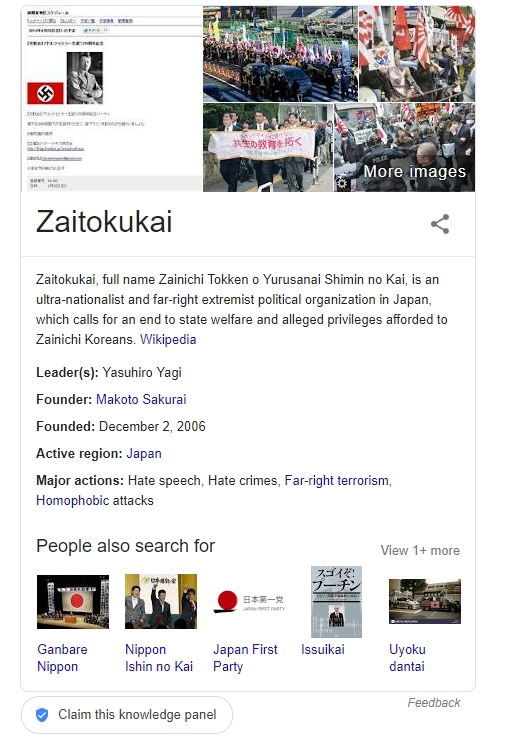
\includegraphics[width=\textwidth]{images/2channel/zaitokukaien.jpg}
  \caption{Search term: Zaitokukai (Source: google.com, taken at July 27, 2019)}
  \label{fig:zaitokukaien}
 \end{subfigure}
  \begin{subfigure}[b]{0.40\textwidth}
  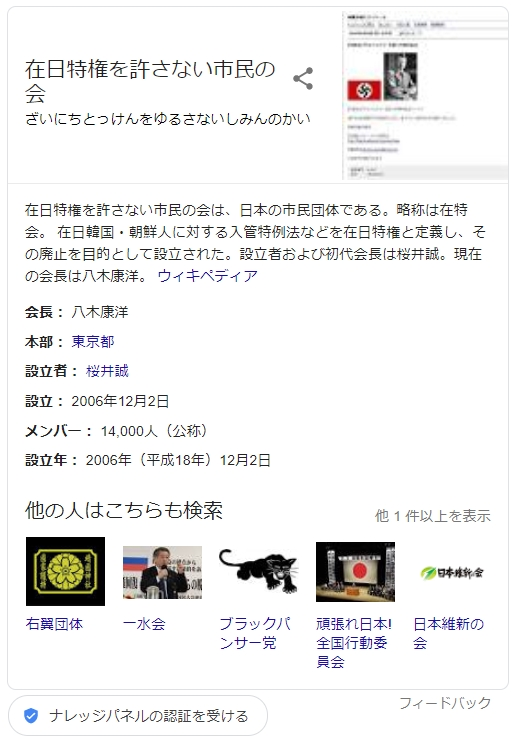
\includegraphics[width=\textwidth]{images/2channel/zaitokukaijp.jpg}
  \caption{Search term: \textit{zaitokukai} (在特会) (Source: google.co.jp, taken at July 27, 2019)}
  \label{fig:zaitokukaijp}
 \end{subfigure}
 \caption{Google Knowledge panels of 'Zaitokukai'}\label{fig:googlezaitokukai}
\end{figure}

This decline of real life manifestations does however not imply a
decline in Netto-Uyoku sentiment. Instead one could argue that the
perceived necessity for such manifestations has also declined due to
fading ideological boundaries between the current rendition of the LDP
and the Netto-Uyoku. Since 2012 the LDP has undeniably taken a shift to
the right, and in that sense, the ACM and the Netto-Uyoku might have
actually achieved their goal of normalizing their neo-nationalist
ideology through wide-spread propaganda, as suggested by Schäfer, Evert,
and Heinrich (\protect\hyperlink{ref-schafer_japans_2017}{2017}).
Furthermore, we have argued in Sakurai's case that he himself is a
product of the discursive processes of right-wing radicalization online.
While there is undeniably ongoing anti-Japanese sentiment amongst
Sakurai's perceived enemies, the carefully curated anti-Japanese
elements dispersed online (purposefully hidden by a supposed leftist
traitorous mass media) make Baudrillard's notion of hyper-reality feel
all the more applicable.

Demographically, Morris-Suzuki
(\protect\hyperlink{ref-morris-suzuki_freedom_2013}{2013}) does not
appear to stray much from the mark either. Tsuji (Tsuji
\protect\hyperlink{ref-tsuji_eng:_2008}{2008}; Tsuji
\protect\hyperlink{ref-tsuji_eng._2017}{2017}) confirms a mostly male
audience active on 2channel and Niconico, and the latter in particular
contains dominantly \emph{otaku} elements, as Azuma
(\protect\hyperlink{ref-azuma_otaku:_2001}{2001}) himself suggested
earlier. The actions of LDP members like Asō Tarō and Abe Shinzō are
then all the more logical.

\chapter{Cybernationalism and Japan --- Connecting the
Dots}\label{cybernationalism-and-japan-connecting-the-dots}

In chapter one, I have suggested that the Netto-Uyoku adhere
ideologically to a form of right-wing populist nationalism (which I'll
further refer to as neo-nationalism). I have further suggested that
media and this form of right-populism sweeping the world are
intrinsically linked. Finally, we can from the very meaning of the
Japanese term Netto-Uyoku (the `Internet Right') draw an implied
importance of the Internet and social media. These loaded statements
lead to several inevitable challenges. Concepts such as ideology,
populism and nationalism (along with such terms as freedom and
democracy) are due to their over-inflation in usage at an increasing
risk of becoming neigh reduced to trending political abstractions; or to
borrow from Laclau's
(\protect\hyperlink{ref-laclau_populist_2005}{2005}, 70) theorization of
semiotics and political identity, empty signifiers. This chapter serves
to build the theoretical framework through which I will interpret the
Netto-Uyoku.

\section{Discourse, Power, Ideology}\label{discourse-power-ideology}

``1. A system of ideas and ideals, especially one which forms the basis
of economic or political theory and policy. 2. The set of beliefs
characteristic of a social group or individual,'' thus defines the
online Oxford Dictionary the concept of ideology.\footnote{\url{https://en.oxforddictionaries.com/definition/ideology}}
Although Terry Eagleton in his \emph{Ideology: An Introduction}
(\protect\hyperlink{ref-eagleton_ideology:_1991}{1991}) agrees that such
a pragmatic view on the notion of ideology is common in public discourse
(albeit with the possibility of an underlying critique: that of the
ideologue having an oversimplified view of the world, and through
indoctrination has a distorted understanding of reality), he does warn,
in light of the historical context briefly sketched below, against one
`Grand Global Theory' or one single comprehensive definition of
ideology; especially one that would contrast ideology with
`pragmatism.'\footnote{``The term ideology, which had originally
  indicated a new science, became a condescending catch-word that served
  to demarcate political enemies. Ideology and ideologue began to
  connote the unwarranted interference of philosophical theory in
  political practices''(Mudde
  \protect\hyperlink{ref-mudde_oxford_2013}{2013}, p:19). These shifts
  are still on-going in today's political discourse and the term is
  often used in a dichotomous relationship to the truth or to a
  ``moderate position'' such as pragmatism. One recent piece by the USA
  political think tank Niskanen Center, for example, uses the terms
  ideologues and extremists interchangeably (Niskanen Center
  \protect\hyperlink{ref-niskanen_center_if_2019}{2019}), while a 2016
  Business Insider article paraphrases Barack Obama as calling Donald
  Trump pragmatic rather than ideological, ``someone who is stringently
  tied to a political philosophy'' (Darcy
  \protect\hyperlink{ref-darcy_obama_2016}{2016}) and Donald Trump, at
  the 73rd Session of the United Nations General Assembly, announced his
  rejection of the ``ideology Of globalism'' (Schwartz
  \protect\hyperlink{ref-schwartz_trump_2018}{2018}).} After all,
following Martin Heidegger's hermeneutic reasoning of interpreting
reality, it would be impossible to identify and judge an occurrence
without a set of preconceived values. Or following Mannheim's Paradox,
analyzing a world-view as an ideology is achieved only from the vantage
point of another ideology
(\protect\hyperlink{ref-eagleton_ideology:_1991}{1991}: p.1, pp221-224).
Actions of the Netto-Uyoku are, intentional or not, ideologically
motivated. By studying the discourse and rhetoric of the Netto-Uyoku, we
can uncover the underlying ideological mechanisms of the Netto-Uyoku,
and by unearthing these processes, we can then understand how its
discourse is formed. Keeping in mind Mannheim's Paradox, that this paper
too is ideologically predisposed,\footnote{The very fact that I am
  applying Marxist critical theory betrays my ideological bias, after
  all, and I therefore cannot claim objective neutrality.} a critical
reading of the Netto-Uyoku's discourse and ideological stances could
help to unravel any contradictions in, and give more insight of, greater
social trends facing our world today.

\subsection{Conceptualizing ideology}\label{conceptualizing-ideology}

Conceptualization of ideology has known many approaches. Historically,
the concept finds its roots in the French Revolution as a positivist
attempt to develop a new scientific framework of Enlightenment ideas
(`the discourse of patterns'), a form of skeptical scientific
materialism (Eagleton
\protect\hyperlink{ref-eagleton_ideology:_1991}{1991}: p.70). Following
Napoleon's attack of the French ``ideologues'' as, in Mudde
(\protect\hyperlink{ref-mudde_oxford_2013}{2013}) (\textbf{Page
number})`s words, ``unrealistic escapism and philosophical reverie,''
ideology has since gone through several shifts in meaning. From a
classical Marxist view, as interpreted by Eagleton
(\protect\hyperlink{ref-eagleton_ideology:_1991}{1991}), ideology too
represented a false or misleading awareness of the human situation.
Ideology was however to be understood as an instrument of those in
control of the means of production. That is to say, steering---whether
intentional or not---the economically subservient class away from a
scientific, objective reality (and hence from what is in the best
interests of the dominated class) with a \emph{false consciousness}, of
one's ability to self-identify as an economic class and express a
political will. Hence maintaining the equilibrium this mode of
production.\footnote{Summed up in the first chapter of Marx' \emph{Das
  Kapital} as ``Sie wissen das nicht, aber sie tun es,'' or in English,
  ``They do not know it, but they do it.''} In other words, classical
Marx' materialist theory places ideology as a superstructure in contrast
to reality within an economic, dialectic basis-superstructure
relationship. The dominant ideology is tied directly to the base, the
mode of production, and visa-versa. On the precondition of being
universally applicable, we might then, for example, view the
\emph{kokutai} (国体) notion or state-Shintoism to be ideological means
for morally \emph{justifying} exploitation (perhaps viewing the
\emph{zaibatsu} conglomerate as part of a Japanese
\emph{bourgeoisie}),\footnote{In \emph{The Japanese Economy}, Flath
  (\protect\hyperlink{ref-flath_japanese_2005}{2005}) refers to the
  \emph{Zaibatsu} as ``at best a kind of \emph{petite bourgeoisie}
  (\protect\hyperlink{ref-flath_japanese_2005}{2005}, 75). Miwa and
  Ramseyer (\protect\hyperlink{ref-miwa_fable_2010}{2010}) in polemic
  fashion dismisses the \emph{Keiretsu} and \emph{Zaibatsu} (industrial
  and financial business conglomerates) in its entirety as fictional
  scapegoats of''Marxist scholars in post-war Japan" and ``populist
  journalists'' (Miwa and Ramseyer
  \protect\hyperlink{ref-miwa_fable_2010}{2010}, 52). He further argues
  a historical growing demand for literature on Japanese economics and a
  lack of Japanese-literate Western economics who have resorted to
  accounts by academics from other disciplines, perpetuating
  conventional Japan-centric claims on \emph{main bank systems} and
  \emph{industrial policy} (Miwa and Ramseyer
  \protect\hyperlink{ref-miwa_fable_2010}{2010}, 54--57).} while in
contrast during the era of the `Economic Miracle', the ideologies of
economic growth and the \emph{nihonjinron} (日本人論) breed of
ethnocentric nationalism would then function to deprive of or obscure
from the subservient class the objective reality; thus maintaining or
legitimizing the \emph{status quo} of society and its economic
structures of exploitation. We see this line of reasoning in the
Alt-Right and Netto-Uyoku-appropriated conspiracy theories of
``red-pilling'' and ``waking up'' (\emph{kakusei} 覚醒 or
\emph{mesameru} 目覚める, a concept Furuya Tsunehiro has referred to as
a matrix-historical viewpoint, \emph{matorikksu-shikan}
「マトリックス史観」). This is a reference to the main character of 1999
science fiction film The Matrix who after consuming a red pill wakes up
to a reality in which humanity is enslaved as a source of energy for a
large machine. The idea of `waking up' or being red-pilled is becoming
aware of a Marxist left-wing elite utilizing their cultural hegemony
over media to brainwash and exploit the ordinary people into believing a
fabricated world-view. This very notion is of course unapologetic
Marxist in nature.

This line of thinking is nevertheless too economically determinist.
Furthermore, failure of Marx' proposed collapse of capitalist society
betrays its rigid scientism. after all, despite hints of a Taisho-era
democracy we cannot pinpoint an exact bourgeois revolution within the
transition from feudalism to capitalism in Japan. Karl Mannheim then
approached ideology as dynamic and being shaped both by the unconscious
assumptions guiding our lives on a \emph{psychological} level, and by
our (social group's) position within social structures, on a
\emph{social} level. For him, this Marxist interpretation of history
\emph{itself} was an ideology; so too changed the pejorative notion of
ideology and grew the idea of a `positive' ideology to counter class
oppression (Dijk and Fabra
\protect\hyperlink{ref-van_dijk_politics_2006}{2006}; Mudde
\protect\hyperlink{ref-mudde_oxford_2013}{2013}: ch.1,ch.3). Since the
early writings on ideology, and with sociological developments such as
the \emph{linguistic turn}, ideology as a concept has seen a wide range
of meanings, deeply entangled with the study of discourse, culture and
politics (Mudde \protect\hyperlink{ref-mudde_oxford_2013}{2013}: ch.1),
with contributions made by amongst others Marxist scholars Louis
Althusser, Georg Lukács (\emph{theory of reification}) and Antonio
Gramsci (\emph{theory of hegemony}), as well as Michel Foucault and
members of the Frankfurt School. Contributions that have helped develop
the relation between the Marxist notion of ideology and the fields of
culture and communication. In his approach to ideology critique,
Eagleton recapitulates top down from its most common to its most
specific usage, in six points the different epistemological perspectives
on ideology (Eagleton
\protect\hyperlink{ref-eagleton_ideology:_1991}{1991}, 28--30; Fuchs
\protect\hyperlink{ref-fuchs_racism_2018}{2018}, 158--59). let us then
observe the following list:

\begin{enumerate}
\def\labelenumi{\arabic{enumi}.}
\tightlist
\item
  Ideology as the ``the general material processes of production of
  ideas, beliefs, and values in social life'' and ``the whole complex of
  signifying practices and symbolic processes in a particular society''
  (Eagleton \protect\hyperlink{ref-eagleton_ideology:_1991}{1991}, p28).
  In other words, a neutral, descriptive definition of ideology as
  \emph{culture}.
\item
  Ideology as the ``ideas and beliefs'' of a ``specific, socially
  significant group or class'' as ``a kind of collective symbolic
  self-expression'' (Eagleton
  \protect\hyperlink{ref-eagleton_ideology:_1991}{1991}, p29). In other
  words, ideology as a neutral \emph{world-view}.
\item
  Ideology as the ``promotion and legitimation of particular interests
  {[}\ldots{}{]} in the face of opposing interests'' and as rhetorical
  discourse, a ``discursive field in which self-promoting social powers
  conflict and collide over questions central to the reproduction of
  social power as a whole'' (Eagleton
  \protect\hyperlink{ref-eagleton_ideology:_1991}{1991}, p29). In this
  definition, ideology begins to be seen in relational, conflictive
  terms.
\item
  Like 3, the ``promotion and legitimation of sectoral interests'' but
  by ``a dominant social power.'' This perhaps in order to
  ``\emph{unify} a social formation in ways convenient for its rulers
  {[}\ldots{}{]} securing the complicity of subordinated classes and
  groups'' (Eagleton
  \protect\hyperlink{ref-eagleton_ideology:_1991}{1991}, pp29-30). This
  definition refines the third definition
\item
  Like 4, ``ideas and beliefs which help to legitimate interests of a
  ruling group or class'' but specifically through ``distortion and
  dissimulation'' (Eagleton
  \protect\hyperlink{ref-eagleton_ideology:_1991}{1991}, p30).
\item
  False or deceptive beliefs ``arising not from the interests of a
  dominant class but from the material structure of society as a whole''
  (Eagleton \protect\hyperlink{ref-eagleton_ideology:_1991}{1991}, p30),
  such as Marx's theory of commodity fetishism. The economic base
  determines the superstructure of ideology.
\end{enumerate}

\subsection{Gramsci, Lukács \& Althusser (Post-War Japan \& The Economic
Miracle)}\label{gramsci-lukuxe1cs-althusser-post-war-japan-the-economic-miracle}

The epistemologically neutral definitions we have seen courtesy of the
Oxford Dictionary fit in the first two descriptions given above, while
the last three are akin the Marxist tradition; the last one in
particular relating to so-called \emph{vulgar} or economically
reductionist Marxism. In these, power is a zero-sum game. The dominant
possession of power invariably reduces the power of the subservient
class. With that in mind, and for importance to this thesis, are the
next generation of Marxists: Gramsci, Lukács and Althusser---three
crucial thinkers in expanding Marxist theory on ideology. Building on
Marx' concept of false consciousness, Lukács theorized class
consciousness as a class-bound ideology obtained through class-level
self-awareness, the result of \emph{reification}. \emph{Reification}
meaning the alienation of the self and a fragmented understanding of the
totality, in the wake of Marx's notion of commodity fetishism and
commodification of labor (Eagleton
\protect\hyperlink{ref-eagleton_ideology:_1991}{1991}, 94--99).

After a failed communist uprising in Italy and in order to explain the
failure of Marx' conception of the inevitable proletarian revolution,
Gramsci recognized culture (or cultural \emph{soft} power) as an
important factor not sufficiently taken in account for in traditional
Marxist theory. Gramsci views the state as a superstructure consisting
of a \emph{political society} and a \emph{civil society}---in other
words, an \emph{integral state} in which the latter is an essential
component for maintaining consent and the former is a means to coerce
and discipline those who don't consent.\footnote{These are concepts by
  the way that Althusser has also systematized as the \emph{ideological
  state apparatus} and \emph{repressive state apparatus}.} Furthermore,
Gramsci coins the notion of \emph{cultural hegemony}, arguing that
consent to the rule of the governing class is a manufactured outcome of
socialization and promulgation of ideology.\footnote{Although not from a
  Marxist school of thought, these topics have also been explored by
  Walter Lippmann in his seminal work \emph{Public Opinion} (1922) and
  Edward Samuel Herman and Noam Chomsky's work on propaganda (an
  ideological form of communication to gain consent) in mass media,
  \emph{Manufacturing Consent: The Political Economy of the Mass Media}.}
More specifically, promulgation through social institutions within the
public sphere of civil society: education, organized religion, the media
industry, and the entertainment industry. While the civil society is in
modern capitalist nations formally not under control of the political
society (notwithstanding that Japan is ranked 67th in the 2019 World
Press Freedom Index),\footnote{Far below Belgium (9), the United Kingdom
  (33) South Korea (41) and the United States (48). This ranking is
  based on among others restrictions of journalism in official press
  rooms (see concept of the `reporters club,' the 記者クラブ \emph{kisha
  kurabu}), strict policies against whistleblowers, and an increasingly
  hostile public climate towards public media (Japan : Tradition and
  Business Interests Reporters Without Borders
  \protect\hyperlink{ref-noauthor_japan_2019}{2019}).} they serve to
impose the state's dominant set of values as ``common sense'': the
values of the dominant class become accepted as that of society in
general. Predominance of the ruling class by coercion is in contrast
restricted to the level of political society, which includes
institutions as the government, police, judicial system and army. In a
modern capitalist state however, civil society and \emph{soft} power
have grown to such an extent that this ``legitimized violence'' has to
certain degrees answer to public consent; which again can be achieved
through the dominant ideology. Yet, if contradictions in the dominant
ideology are too great, the manufacturing of consent becomes
unsustainable. In other words, this leads to a \emph{hegemonic crisis}.

For Althusser, ideology was an \emph{unconscious}, discursive and
material process; assimilated and reproduced through cultural practices
in the ideological state apparatus; with little space for human agency.
Gramsci does however see room for this in civil society. For Gramsci,
ideology does have value. He further coins the concept of
\emph{subaltern} (a term crucial in post-colonial studies)\footnote{In
  post-colonial theory, the concept of the subaltern refers to those in
  the margins of colonial society, lacking of agency and being forced to
  resort to speak the colonial oppressor's language. Crucial early works
  on the topic include Edward Said's \emph{Orientalism} (1978) and
  Gayatri Chakravorty Spivak's deconstruction \emph{Can the Subaltern
  Speak?} (1983), which criticizes the practice of interpreting the
  Other through western methodology. Something I feel I am guilty of,
  writing this very paper on Japanese \emph{digital nationalism} using
  mostly western traditions of academic theory and methodology as
  universally applicable. I find some irony too in basing my Japanese
  resume on my English manuscript, neither of which are my native
  languages.} to refer not just to those lacking in economic and
political power (such as peasants and the proletariat), but those whose
very cultural or social identity is on the fringes of the dominant
ideology. Those whose history is overshadowed by that of the ruling
class and who are denied the right to make one's own culture and
historical narratives. Yet in these fringes is an opening to develop a
subaltern consciousness, a \emph{sub-culture}. For revolution to be
successful, it is therefore first necessary for those groups to
dismantle the cultural hegemony by developing one's own organic ideology
(a dialectic process of an ``ideological struggle'' with the hegemonic
ideologies) unifying a `collective will' as class-consciousness and
producing a counter-hegemony. Only after ascertaining a
counter-hegemonic dominance on civil society could the subservient
classes succeed in coercive action over the political society (Gramsci
and Hoare \protect\hyperlink{ref-gramsci_selections_1985}{1985}: p.47,
pp.210-238).\footnote{These concepts have been translated as \emph{War
  of Position} and \emph{War of Maneuver} (Buttigieg
  \protect\hyperlink{ref-buttigieg_gramsci_1995}{1995}; Gramsci and
  Hoare \protect\hyperlink{ref-gramsci_selections_1985}{1985}: p.46). It
  must be noted that this part of Gramsci's reasoning has since gained
  renewed popularity and seen appropriation by both Identitarian
  movements and the Alt-Right. Social institutions education and the
  mass media are seen as platforms for manufacturing consent to a
  hegemonic left-wing or globalist ideology, and the notion of Gramsci's
  counter-hegemony is re-framed as \emph{metapolitics} (Stein
  \protect\hyperlink{ref-stein_jeff_2018}{2018}). Belgian populist
  right-wing party member Dries Van Langenhove claims his Identitarian
  youth movement Schild \& Vrienden to function as a vehicle of
  metapolitics (NWS \protect\hyperlink{ref-nws_van_2018}{2018}), and
  previous Vlaams Belang leader Filip de Winter added that ``The
  methodology Gramsci promoted is the right one'' (``De methodiek die
  Gramsci aanprees, is de juiste'') (Ceulaer
  \protect\hyperlink{ref-ceulaer_6_2016}{2016}).} Gramsci calls this
\emph{passive revolution} (Gramsci and Hoare
\protect\hyperlink{ref-gramsci_selections_1985}{1985}, pp106-120). In
the case of a crisis of hegemony as mentioned above, the dominant class
has no means but to either rely on coercion through the political
society, or to consolidate oppositional movements in civil society (the
passive revolution). Ideology for Gramsci is a specific historical
phenomenon (a ``historicist'' approach in contrast to ``scientific''
Marxism) and observable both on a micro- and macro-scale. On an
individual level, ideology is a ``lived, habitual social practice
\ldots{} the unconscious, inarticulate dimensions of social
experience''; on a collective level it is that of social institutions
(Eagleton \protect\hyperlink{ref-eagleton_ideology:_1991}{1991}, p115).
Perry Anderson\footnote{Brother of Benedict Anderson, who gained fame
  with his notion of socially constructed ``imagined communities''
  (\protect\hyperlink{ref-anderson_imagined_2006}{2006}).} builds on
this. Whereas Gramsci locates cultural hegemony in civil society alone,
Anderson finds hegemony in political society, ``for the political form
of the capitalist state is itself a vital organ of such power,'' and
reasons that the institutions of civil society play a complementary role
to hegemony (Eagleton
\protect\hyperlink{ref-eagleton_ideology:_1991}{1991},
112--13).\footnote{In this paper's introduction, I noted the Alt-Right's
  infatuation with Japan in particular. Asking why, one might look at
  war-time relations between the far-right in the West and Japan. In
  Fukushima's mount Iimori, for example, I examined both an
  archaeological column of Pompeii, donated by Italian fascist leader
  Mussolini, and a 1930s German donation in the form of a black granite
  plate with an Iron Cross--as form of praise for the
  \emph{bushido}-related war-time propagandistic media-event of the
  White Tiger Company military unit (\emph{Byakkotai}, 白虎隊), the
  story of 19 teenagers committing ritual suicide after mistakenly
  believing their castle had fallen during the Bosshin War. Perhaps in
  more recent memory, one other answer could be found in a dialectic
  processes of cultural hegemony between Japan and the West. With the
  widespread `80s narratives of Japan as economic powerhouse and the
  growing cultural \emph{soft} power of Cool Japan, many a page were
  written on the \emph{Japanese model} (see for example Chalmers' 1982
  \emph{MITI and the Japanese Miracle}), and thus a window opened to
  sell Japan's hegemonic ideology of \emph{nihonjin} 日本人論 style of
  (ethno-)nationalism to the West.}

Some concrete examples of this reasoning. If orthodox Marxism were to
view the contradictory nature of increasing student debt in the United
Stages and the ideological narratives of neo-liberal
capitalism\footnote{``In reality, it is a material political and
  ideological formation that has the function of managing the new mode
  of production of a transnational High-Tech Capitalism'' (Rehmann
  \protect\hyperlink{ref-rehmann_bernie_2016}{2016}).} as a trigger for
working class awareness and the inevitable overthrow of capitalism, then
in Gramsci's interpretation, civil society would be the stage for
counter-hegemonic processes in passive revolution. 2011 saw widespread
resentment directed at Wall Street in the populist Occupy Wall Street,
with ideological slogans as ``We are the 99\%'' (Rehmann
\protect\hyperlink{ref-rehmann_bernie_2016}{2016}). In 2019, politicians
Bernie Sanders, Elizabeth Warren and Alexandria Ocasio-Cortez are
running on a counter-hegemonic platform to cancel student debt.
Likewise, although the democratic impact of the 1994 electoral system
reforms in Japan is questionable considering the near constant dominance
of the Liberal Democrat Party on national politics since (Komatsu
\protect\hyperlink{ref-komatsu_first_2017}{2017}), the 1993 Japanese
general election and fall of the 1955 system\footnote{\emph{55-nen
  taisei} (55年体制). An electoral system of Single Non-transferable
  Vote in which the Liberal Democratic Party (LDP) held political
  dominance over the Japan Socialist Party (JSP).} could also be read
through this lens. When Japan, as elsewhere, entered a late-capitalist
phase of mass consumerism, different contradictions arose. Although not
explicitly referring to Gramsci or Marxist traditions of ideology, the
language of Dower et al.
(\protect\hyperlink{ref-dower_peace_1993}{1993}) in his narrative
assessment of the New Left and late '60 political movements certainly
seem to suggest such logic as well. As Dower states, the growth of Japan
as a cultural and economic powerhouse brought to light contradictions in
society---the \emph{San Francisco System}, the ambiguous position of
Okinawa and environmental issues (mercury poisoning in Minamata) to name
a few; pitting ``liberal and left-wing critics against the dominant
conservative elites'' and introducing ``a more radical anti-imperialist
critique to the discourse on peace and democracy.'' In light of rapid
economic growth, hegemonic ideologies of nationalism, capitalism, peace
and democracy retained a strong grip on public consent, or as Dower et
al. (\protect\hyperlink{ref-dower_peace_1993}{1993}) puts it, the
``conservative hegemony-the bedrock of the 1955 System-continued to rule
japan'' (Dower et al. \protect\hyperlink{ref-dower_peace_1993}{1993},
5--6,p.21). Nevertheless this counter-hegemonic shakes society in the
late '60s.

\begin{quote}
``It is estimated that between 1967 and 1970 alone, more than eighteen
million Japanese took to the streets to protest the war in Vietnam and
demand the reversion of Okinawa to Japan. Uncounted others were involved
in the university struggles and citizens' movements against the ravages
of the growth-oriented state. As elsewhere,''people's power" entered the
Japanese lexicon at this time as a legitimate and essential alternative
to bourgeois parliamentary politics; and, as elsewhere, the theory and
practice of ``people's power'' ranged from peaceful protest to wanton
violence. By the mid-1970s the nationwide people's movement was
moribund, but it left as legacies the memory and experience of
grass-roots mobilization that could be evoked in more particularistic
causes thereafter." (Dower et al.
\protect\hyperlink{ref-dower_peace_1993}{1993}, 22)
\end{quote}

This was a period of hegemonic crisis, but one that in its aftermath did
leave a considerably sour aftertaste in the mouths of many. Communists
groups associated with New Left thought, such as the Japanese Red Army
and the East Asia Anti-Japan Armed Front, proceeded directly to direct
action and vise-versa so did the political society too respond with
violence. Furthermore, in light of economic growth and relative public
wealth, the hegemonic ideologies of economic and ethnic nationalism
(what Dower et al. (\protect\hyperlink{ref-dower_peace_1993}{1993})
coins a ``late-Showa cult of exceptionalism''
(\protect\hyperlink{ref-dower_peace_1993}{1993}, 6)) had despite high
profile political scandals as the Lockheed bribery thus far helped
retain a strong, manufactured grip on consent. Nevertheless, with the
collapse of the bubble economy so too did contradictions in the
dominant, hegemonic ideology once again become unearthed (Akio Morita
and Shintaro Ishihara's 1989 essay \emph{The Japan That Can Say No} has
not aged particularly well), renewing distrust in established politics
and the political system behind it. In other words, the political reform
of the 1955 System by temporarily allied political outsiders in 1994 was
the logical outcome of an increased alienated Japanese civil society.

\subsection{The Frankfurt School \& Post-Ideology (The Lost
Decades)}\label{the-frankfurt-school-post-ideology-the-lost-decades}

The Frankfurt School of Critical Theory furthers the theoretical
approach to how culture shapes ideology. In particular, Adorno and
Horkheimer's Dialectic of Enlightenment

Habermas: public sphere

Adorno: the culture industy

This line of reasoning is in itself of course highly ideological and if
any of this sounds unapologetically populist, that is no coincidence. I
consider this logic an important tactic of what I call \emph{digital
populists}, populists focusing on cultural-ideological warfare on the
Internet and whose rhetoric is shaped by sub-cultures online. I maintain
that this Gramscian understanding of ideology and hegemony is beneficial
in understanding the processes of reasoning behind populist,
neo-nationalist (and ultimately, `cyber-nationalist') ideology.
Moreover, the open and public nature of the Internet and social media
would present an ideal public space for the under-represented to form a
cultural identity and engage in ideological struggle with the hegemonic
dominant ideology. The rise of online \emph{influencers} using social
media such as YouTube, Niconico, Twitter, Instagram and Facebook to
spread politically inspired messages, and right-wing populists utilizing
this medium to sell a narrative of revolution, certainly seem to suggest
so. Furthermore, As I will expand on in the next chapter, its very
creation is commonly framed as being rooted in the American libertarian
counter-culture movement of the sixties, after all.

The debate on ideology far from stopped since. Francis Fukuyama, for
example, claimed in his essay \emph{The End of History?} that we have
reached a post-ideological world in which western liberal democracy was
the end-point of ideological evolution, an idea that could not be
improved upon. On the other side, and furthering Lukács' ideas on
alienation due to the increased importance of commodity fetishism in
capitalist society, Žižek views late-capitalist cynicism as inherent to
modern-day ideology, summarized best as ``they know very well what they
are doing, but still, they are doing it.'' We are aware of the
contradictions, of the false consciousness, but we renounce it only in
cynical subversion (\protect\hyperlink{ref-zizek_mapping_2012}{2012},
18, pp312--5).

\section{Neo-Nationalism}\label{neo-nationalism}

Can we then interpret this world-wide growth of neo-nationalist
movements as counter-hegemonic process?

\subsection{Populism}\label{populism}

How then are we to understand populism? Open just about any recent
article on politicians such as Donald Trump, Bernie Sanders, Viktor
Orbán, Corbyn, Jair Bolsenaro or Matteo Salvini and the possibility is
high any of them will have been name-called a populist, disregarding any
dissimilarities in either political agenda or geographical situation.
Often used in a pejorative fashion, there is however little explanation
if any at all offered in those takes, and with an unprecedented soar in
the frequency of usage of this term in Western discourse (a Google
Trends search for populism both worldwide and in Japan over the past 10
years, as illustrated on \textbf{figure \ref{fig:populism-gt}}, reveal a
worldwide rise of public interest in populism correlating to the
political shifts referred to earlier),\footnote{Although these worldwide
  trends reflect on Japan, they are preceded with a short but strong
  spike of interest in both July 2011 and August 2012, suggesting the
  concept of populism had penetrated Japanese public discourse a fair
  bit earlier as on a global scale. A period, barely a year after the
  devastating 2011 Tōhoku earthquake in which political outsiders
  Shintaro Ishihara and Hashimoto Taro were making headlines, current
  prime minister Abe Shinzo was staging his political comeback, Tsuneo
  Watanabe, who was once called Japan's most powerful media baron
  (Onishi \protect\hyperlink{ref-onishi_shadow_2006}{2006}), publishes a
  book warning against the dangers of populist nationalism (Watanabe
  (\protect\hyperlink{ref-watanabe_anti-populism_2012}{2012})), and
  literary critic Azuma Hiroki gains renewed success with his
  publication of \emph{ippan-ishi 2.0} (General Will 2.0, 一般意志2.0).}
the term populist is increasingly used interchangeable or combined with
demagoguery.\footnote{One \emph{The Huffington Post} article, for
  example, referred to Roman politician Publius Clodius Pulcher as ``the
  Trump of Ancient Rome, a Populist Demagogue Who Helped Bring Down the
  Republic'' (Freeman, professor, and author
  \protect\hyperlink{ref-freeman_meet_2016}{2016}).}

\begin{figure}[!htb]
 \centering
 \caption{\label{fig:populism-gt} The Google Trends of Populism Worldwide \& Japan (10 Years).}
 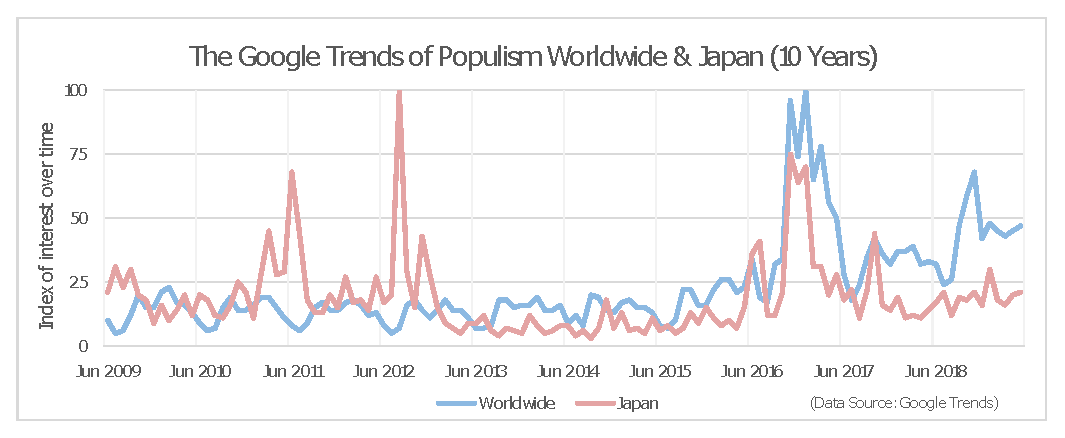
\includegraphics[width=0.95\textwidth,trim=4 4 4 4,clip]{images/populismtrends.eps}\end{figure}

\subsubsection{Theory}\label{theory}

\subsubsection{Populism in
Japan(日本型ポピュリズム)}\label{populism-in-japanux65e5ux672cux578bux30ddux30d4ux30e5ux30eaux30baux30e0}

http://www.tokyoreview.net/2018/09/antonio-inoki-fighting-spirit-diplomacy/

\subsection{Nativism}\label{nativism}

Vanaf hier specifiek over rechts nu en neto-uyo praten

\subsection{Nationalism}\label{nationalism}

\section{Cyber-Nationalism}\label{cyber-nationalism}

https://en.wikipedia.org/wiki/Cyber-nationalism

\subsection{The Medium is the Message}\label{the-medium-is-the-message}

Despite some cultural lag, there are now many theoretical options to
approaching the Internet, new media, and politics. In an early stage,
Rimmer and Morris-Suzuki (1999), following sociologists Kumon Shumpei
and Masuda Yoneji's writings on a `teledemocracy', take a utopian view
and predicted the Internet would serve democracy by fundamentally
altering its users thinking patterns and leading to a power-shift away
from mass-media. Recent debate on the Internet's role in populist
politics in East-Asia (Youngmi Kim 2009, Azuma Hiroki 2011, Tamura en
Kobayashi 2014) have instead taken a distinct dystopian turn, employing
such terms as `the People's Will 2.0', and again arguing that due to the
very nature of computer-mediated communication and social media, with
traits such as anonymity, filter-bubbles and so-called `echo-chambers',
the individual `will' has been reduced to a general `will' led by
emotion rather than rationality. Thus, following this logic, Internet as
an open medium for communication would become an invaluable tool for
political leaders utilizing a populist narrative.

Paradigm shift: postmodernist fragmentation due inhibiting the linear
reading exerpience

\subsection{Japanese Internet}\label{japanese-internet}

The development of the Internet in Japan has a similar history as in the
United States and Europe, starting with universities developing
technology to interlink academic papers. As the ``first nationwide
noncommercial computer network'' in 1984, JUNET (Japan
University/UnixNETwork) linked Tokyo University, Keio University and the
Tokyo Institute of Technology (Aoki
\protect\hyperlink{ref-aoki_virtual_1994}{1994}). According to Barubora
and Sayawaka (\protect\hyperlink{ref-barubora_eng:_2017}{2017}), the
loosening grip of government policy in 1985 led to the consequent
adaptation of bulletin board systems (BBS) for computer-mediated
communication between hobbyists in Japan. Through translations in
technological magazines,\footnote{Such as Mitsuhiro Takemura's
  メディア・エクスタシー (\emph{media ekusutashī}, `Media Ecstasy') and
  Kazuhiko Nishi's 『ASCII』 (\emph{asukī}, アスキー) and its spin-off
  『ログイン』 (\emph{roguin}, LOGiN), although the latter gradually
  evolved into a solely gaming-centered magazine (the now famous
  \emph{Famitsu}). Its founder, Nishi Kazuhiko is mostly known for his
  work on the Japanese desktop-computer PC-8001, and the development of
  the MSX in a joint project with Bill Gates.} the ideology of American
west coast voices crucial to the rise of Silicon Valley becomes known in
Japan as \emph{shisō nishikaigan shisō} 西海岸思想 or \emph{Karuforunia
shisō} カリフォルニア思想 (West Coast Thought or California Thought): an
ideology that envisions increased participation in democracy through the
development of IT and computer science. In his narrative on the
development of computers and the Internet, John Markoff echoes this
connection of the libertarian hackers-ethos to '60s counterculture
(\protect\hyperlink{ref-markoff_what_2005}{2005}). Barubora and Sayawaka
(\protect\hyperlink{ref-barubora_eng:_2017}{2017}) argue that while, as
Markoff too states, early rhetoric on the Internet in the united states
is built on newsgroups discussing political activities and usages of the
medium,\footnote{Such as John Gilmore's \emph{Cypherpunks} mailing list,
  who later co-founded the Electronic Frontier Foundation with John
  Perry Barlow, author of the 1996 \emph{A Declaration of the
  Independence of Cyberspace}.} in contrast were Japanese mailing lists
and BBS then primarily built around niche sub-culture topics
(\protect\hyperlink{ref-barubora_eng:_2017}{2017}, ch.1). Aoki
(\protect\hyperlink{ref-aoki_virtual_1994}{1994}) too argues that early
adaption was associated with \emph{otaku} (\emph{otaku-zoku}, オタク族,
a term that roughly in this timespan came to denote those with obsessive
interests in sub-culture topics) and less accessible to the public due
to the difficulty of encoding Japanese characters on the Internet; early
communication had to be written with the Latin script.\footnote{Which
  incidentally lies at the root of particular now `mainstream'
  \emph{net-slang}, such as the common usage of multiple letters `w' as
  signifier of humor (the loose equivalent of the now rather outdated
  `\emph{lol}', laughing out loud). As abbreviation of `(笑)'
  (\emph{wara}, `to laugh'), this \emph{slang} saw its first usage on
  platforms that required Japanese to be written with the Latin script.}

(Azuma \protect\hyperlink{ref-azuma_otaku:_2001}{2001}) has argued the
same, claiming that from the beginning of computer mediated
communication (CMC) in Japan in the '80s onwards, the discourse on
Japanese internet has been shaped by \emph{otaku}; not just through
websites and bulletin boards through references to Japanese animation or
video-games dispersed on a technical level as well (such as in the
naming of FTP-sites or sample sentences in manuals for word or
spreadsheet software) (\protect\hyperlink{ref-azuma_otaku:_2001}{2001},
4)

\section{Model}\label{model}

blabla

\begin{table}[!htb]
\footnotesize
\centering
\setlength{\tabcolsep}{5pt}
\caption{Model of Cyber-Nationalism Applied to Netto-Uyoku}\label{tab:modelcybernationalism}
\scalebox{0.8}{
\begin{tabular}{ll}
\toprule
Ideology&Topics\\
\midrule
Nationalism&Identity, Japan, Patriotism\\
Nativism&Foreigners, Koreans, China\\
Revisionism&Pacific War, Comfort Women, Territorial Disputes\\
Populism&Mass Media, Truth, (Left Wing) politics\\
Digitalism&Internet, 2channel, matome\\
\bottomrule
\end{tabular}
}
\end{table}

(Rimmer and Morris-Suzuki
\protect\hyperlink{ref-rimmer_japanese_1999}{1999})

\section{Conclusion}\label{conclusion-1}

This paper takes a critical approach to ideology, basing itself
primarily on the work of Gramsci and thinkers aligned with the Frankfurt
School of critical theory. Thus in this paper I view ideology as a
world-view rooted in class-conflict; and in capitalist nations that rely
on consent over coercion, as a means to consolidate power. Consolidating
power over civil society as done by those in control of the political
society (the `elite' or establishment) through disseminating ideology
(by means of popular culture and mainstream media: the hegemonic
ideology). Contradictions in society, a consequence of the capitalist
nature of commodity fetishism, lead to alienation among exploited
classes and therefore to class-awareness and an opening for
counter-hegemonic processes in civil society. This reasoning is a strong
element of populist rhetoric and neo-nationalists. I adhere to Mudde
(\protect\hyperlink{ref-mudde_oxford_2013}{2013})`s definition of
populism as a thin-centered ideology based on the antagonizing of an
'elite' in function of a homogeneous `will' of `the people'. Right-wing
populists view the `elite' in this case as primarily a left-wing entity
utilizing the media to spread manufactured consent through a \emph{fake}
world-view. In this narrative the populists \emph{are} the
counter-hegemonic forces. They utilize alternative means in
civil-society to appeal to `the people', the exploited classes that are
more often than not defined based on nationalist ideologies: ethnic
background or cultural values (i.e.~Judeo-christian values). This
\emph{fake} world-view borders on a nativist conspiracy theory wherein
globalist values of the elite lead to clashes of culture and the
disintegration of `the people's' best interest.

What the French fachosphère, the Japanese Netto-Uyoku and the American
Alt-Right have in common is exactly that: a neo-nationalist ideology of
populism, nationalism and nativism. I argue however a difference between
those that adhere to this ideology and utilize the Internet purely for
organizational means (ie. protest marches), and \emph{netizens} as a
sub-culture adhering to an ideology of Internet as a `new frontier'

For them, however, the Internet forms an escape in the form of a `new
frontier'; one that ought to be free from elite interference. With some
violent exceptions, there is a difference between

In other words, what I have defined as cyber-nationalism.

If self-perceived contradictions in society (such as immigration and
terrorism) brought about a wave of right-wing populism with 2016 as a
pivotal year, then 2009 - 2011 could be considered the same for Japan.
Blatantly populist politicians as Shintaro Ishihara and Hashimoto Toru
gain renewed fame,

\chapter{The Anatomy of Japanese Cyber-Nationalism ー From 2channel to
Wikipedia}\label{the-anatomy-of-japanese-cyber-nationalism-ux30fc-from-2channel-to-wikipedia}

I illustrated in the second chapter that Netto-Uyoku are often
associated particularly with 2channel, Niconico and with its more recent
rise of usage in Japan, with Twitter as well (Katayama
\protect\hyperlink{ref-katayama_2-channel_2007}{2007}; Tsuji
\protect\hyperlink{ref-tsuji_eng:_2008}{2008}; Sakamoto
\protect\hyperlink{ref-sakamoto_koreans_2011}{2011}; Murai
\protect\hyperlink{ref-murai_net_2012}{2012}; Yasuda
\protect\hyperlink{ref-yasuda_eng:_2012}{2012}; Morris-Suzuki
\protect\hyperlink{ref-morris-suzuki_freedom_2013}{2013}; Taka
\protect\hyperlink{ref-taka_twitter_2015-1}{2015}\protect\hyperlink{ref-taka_twitter_2015-1}{b}).
Furthermore, all of these belong to the top visited websites in Japan,
with the latter two dominantly fixed in the top ten.\footnote{For more
  information, I refer to \textbf{table \ref{tab:50mostpopjp}}.} In the
previous chapter I have also brought up McLuhan's argument that the
content of the message is itself intrinsically shaped by the vessel
through which it is delivered. Following this argument through in the
age of online social media, Lev Manovich argues that software now takes
a central position in our interaction with the world around us
(\protect\hyperlink{ref-manovich_software_2013}{2013}). As someone
creates a potentially viral image intended for political persuasion and
posts it online, they might do so using their laptop computer to edit
different layers of the image through image-editing software as
Photoshop. Next they might use Chrome as a browser to interpret and
visualize the semantic text of the World Wide Web (HTML), and upload the
image on a platform as Twitter or 2channel. They have to adhere to the
limits required on image-size and length of text, and preferably add
symbols for interconnection or recognition to gain a wider reach (using
hash-tags, the @ sign, or \emph{trip-code} identifiers on
pseudo-anonymous Bulletin Board Systems). Combined, these are a great
amount of different interfaces for communication. Azuma
(\protect\hyperlink{ref-azuma_otaku:_2001}{2001}) expresses similar
reasoning. Whereas the content of other media has one final represented
form, data on the World Wide Web is determined by software. A web-page
built using the HTML syntax will represent the contents in a different
fashion depending on the software and hardware it is opened with, and
reveals the underlying structural composition when opened with a
text-editor instead of a browser. Furthermore, similar to the non-linear
structure of games, non-linear paths are an intrinsic element of the
world wide web's hyper-connectedness
(\protect\hyperlink{ref-azuma_otaku:_2001}{2001}, ch.3).

Since the effective start in the mid 2000s of what Tim O'Reilly coined
the \emph{Web 2.0}---a participatory web based on interactive
collaboration and user-generated content---as well as the onset of
machine learning and artificial intelligence in generating semantically
interlinked content, over a decade has passed for social media and its
hyper-extended \emph{hyper-connectedness} to mature within our lives.
Based on my theoretical framework in the previous chapter, I approach
this chapter through a mixed methods critical content analysis applied
to social media, attempting to bring to light from a semiotic
perspective how the Netto-Uyoku reinforce and disperse ideological
narratives on the Internet. While it is hard to ignore major platforms
as YouTube, Twitter and 2channel, I will focus particularly on two
less-documented forms of Internet-based media in Japan:
\emph{2channel}-based \emph{matome} curated aggregation websites and
Wikipedia. The former as a a means to disperse to a greater audience a
selected sample of certain sub-categories as supposedly representative
of the Internet \emph{vox populi}. The latter, an open and collaborative
encyclopedia built on hyper-links, is both a prime example of Azumi's
non-linear and endless structure inherent to the world wide web and,
more concretely, gives us through its revision history insights in how
and by whom persuasive narratives are formed.

\section{\texorpdfstring{2channel \&
\emph{Matome}-blogs}{2channel \& Matome-blogs}}\label{channel-matome-blogs}

Although I cannot dismiss previous literature in tracing the
\emph{Netto-Uyoku} and their rhetorical methods back to
2channel,\footnote{Take for example the suffix 「~ニダ」 \emph{nida} as
  a pejorative expression in imitating someone with an ethnic Korean
  background.} it would be unwise to dismiss those platforms in their
whole as one homogeneous, even toxic community (with at their peak
millions of messages per day).\footnote{Katayama
  (\protect\hyperlink{ref-katayama_2-channel_2007}{2007}) reported in
  2017 2.7 million messages per day spread over 800 different
  categories. Whereas \emph{2channel} was in 2017, a decade after that
  report, still the \nth{18} most visited website in Japan (Poppe
  \protect\hyperlink{ref-poppe_digitaal_2017}{2017}, 15), in its current
  renamed state as 5channel it has since dropped to \nth{43} position.}
The technical base behind 2channel was created in 1999 based on the
structure of early Usenet-inspired Bulletin Board Systems \emph{ayashī
wārudo} あやしいわーるど (1996, lit. `Strange World') and \emph{amezō
rinku} あめぞうリンク (1997), purposed as a text-only multi-threaded
anonymous messaging board
(\protect\hyperlink{ref-barubora_eng:_2017}{2017}, ch.2). These were
subsequently the origin for the more graphically-oriented \emph{Futaba
Channel}, the software base on which \emph{4chan} is based on. While
correctly identified as strictly anonymous, users have the option to
register a personal identifier (a trip-code). Moreover, messages
(\emph{posts}) have a numeral ID used when reacting to another post, and
within one \emph{thread} (a conversation on one particular topic) users
often have a fixed ID to keep some consistency in communication. A
thread has a limit of 1000 posts before it is `archived' (meaning no new
reactions can be placed) and users need to create a follow-up thread.
Similar to the structure of news websites, those approximately 800
boards are thematically divided (including such topics as news, society,
sports, idols and video-games). A 2channel ranking-site (based on the
amount of threads and replies within a certain timespan)\footnote{See
  \url{http://2ch-ranking.net/}.} consistently places boards belonging
to the news section on top, as well as several boards dedicated to idol
culture.

One trend that accompanied the growth of 2channel is the appearance of
so-called \emph{matome}-sites. Those are curated aggregation websites
based around particularly popular (\emph{viral}) threads on 2channel
(and since the early 2010s other social media platforms such as
Twitter). The curator manually collects the material s/he deems most
relevant to the viral topic in question---either as representation of
public opinion, or for its comical value---and is usually accompanied
with a particularly appealing title (what is in English colloquially
known as `clickbait') and a short personal comment. A common trait of
those \emph{matome}-sites is the usage of private advertising or
services such as Google's Adsense for the pursuit of financial
profit,\footnote{This is pejoratively known as \emph{afikasu}
  アフィカス, a contraction of \emph{afiriēto} アフィリエイト and
  \emph{kasu} カス, loosely translated as `affiliate-tainted'.} and one
of the larger subsections (boards) of 2channel, \emph{Nyūsu sokuhō
(kenmō)} ニュース速報 (嫌儲)\footnote{A subdivision of the
  \emph{Breaking News} boards. 嫌儲 \emph{kenmō} is a word play on 嫌韓
  \emph{kenkan} (lit. `Hate Korea') and translates to `Hate Profit'. The
  URL itself \url{https://5ch.net/poverty/} itself contains an English
  language pun.} started in protest of such curated aggregation sites
and may by terms of service not be aggregated.

\begin{figure}[!htb]
 \centering
 \begin{subfigure}[b]{0.95\textwidth}
  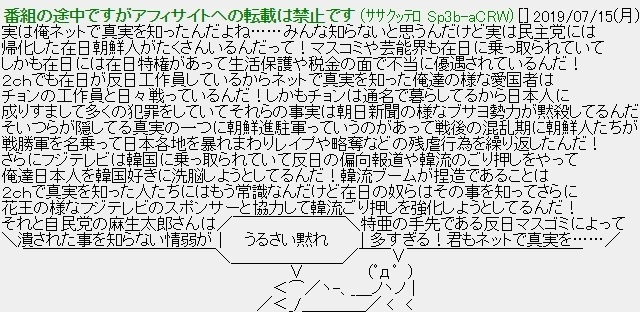
\includegraphics[width=\textwidth]{images/2channel/anti-aa.jpg}
  \caption*{\textbf{Above}: "In fact, I learned the truth on the Net... I don't think many know this but in fact there are a lot of naturalized Koreans in the LDP! The media and the entertainment world have also been taken over by Zainichi Koreans, and they enjoy privileged rights unfairly favored in terms of welfare and taxes! Patriots like us who learned the truth on the net are fighting daily with anti-Japanese \textit{chon} agents because they have infiltrated even 2ch! Moreover, because \textit{chon} use common names, they commit many crimes pretending to be Japanese, and these facts are being suppressed by the \textit{filthy leftists} like the \textit{Asahi Shimbun}! One of the facts they hide is that that during the post-war chaos, Zainichi Koreans pretended to be part of the victorious army and ran around all over Japan committing atrocities such as rape and looting! Furthermore, Fuji TV is being taken over by South Korea, and try to brainwash Japanese people into liking Korea by biased anti-Japanese reporting and airing the Korean Wave! It is common sense for the people who learned the truth on 2ch that the Korean Wave is forged, but Zainichi Koreans know this as well and try to further cooperate with sponsor of Fuji TV like Kao Corporation to enforce and strengthen the Korean Wave! Moreover many people have inadequate access to information that the LDP's Taro Aso was thwarted by the anti-Japanese garbage media, a puppet of Anti-Japanese Asian countries. You too should learn on the Net..." \textbf{Below}: "So noisy, shut up!"\newline (Screenshot by author. Source: leia.5ch.net/poverty/)}
  \label{fig:aajp}
 \end{subfigure}
 \caption{ASCII Art (AA) parodying Netto-Uyoku}\label{fig:aa}
\end{figure}

In a July 15, 2019 thread on this board, users discuss if and why there
are less expressions of Netto-Uyoku discourse on \emph{kenmō}. There is
no consistent political ideology amongst its users (who refer to
themselves as \emph{kenmomen} ケンモメン or 嫌儲民), but in an
interesting group dynamic there is a perception of the other \emph{nyūsu
sokuhō} boards as their cultural Other, with an overall resistance to
profit-seeking aggregation sites and writers targeting the medium they
identify with.\footnote{Referred to as \emph{biji-uyo} (ビジウヨ, an
  abbreviation of business-right, \emph{bijinesu-uyoku} ビジネス右翼)
  and \emph{sutema sōdō} (ステマ騒動, stealth-market unrest).} Through
somewhat serious discussion on nationalism and ideology (along an
occasional conspiracy theory),\footnote{Several reactions claim
  mind-control (i.e.~Marx' notion of `false consciousness') by the
  left-wing and ethnic outsiders. See for example: .``..In spite of
  being controlled by the baby boomer leftists, and Zainichi Koreans and
  Chinese'' (\emph{zainichi chūgokujin, zainichi kankokujin, dankai
  sayoku ni kontorōru saretekita baka no kuse ni yo}
  「在日中国人、在日韓国人、団塊サヨクにコントロールされてきたバカのくせによ」).}
several users echo the 2011 earthquake as a trigger for psychological
cravings for positive nationalist self-reinforcement and view
\emph{matome} blogs as one such tool. Conclusively, these
\emph{kenmomen} dislike profit-seeking \emph{matome} blogs and
marketers, therefore they reason they have not become \emph{Netto-Uyoku}
themselves (which are often subject to parody, as illustrated on
\textbf{figure \ref{fig:aa}}).\footnote{An earlier trend on 2channel and
  similar message-boards was the usage of text-based artwork (AA, ASCII
  Artwork), the Japanese variant of the viral imagery referred to as
  \emph{memes}. While somewhat out of fashion, they are now recycled in
  an ironic manner.} One anonymous user summarizes their answer to the
thread's question as follows (5ch.net
\protect\hyperlink{ref-5ch.net_eng._2019}{2019}):

\begin{quote}
「右翼とか左翼以前に世の中の天邪鬼なのがネットの主流だから\newline
ネトウヨがまだ頭が良いと思われていた頃はテレビや世間が左寄り\newline
今はテレビや世間がネトウヨやっているから俺たちが左寄りでバランスを取らないといけない\newline
って言う潜在意識があるんだよ」
\end{quote}

\begin{quote}
``\emph{Uyoku toka sayoku izen ni yononaka no amanojakuna no ga netto no
shuryūdakara\newline neto-uyo ga mada atamagaii to omowa rete ita koro
wa terebi ya seken ga hidariyori\newline ima wa terebi ya seken ga
neto-uyo yatte irukara oretachi ga hidariyori de baransu o toranaito
ikenai\newline tte iu senzai ishiki ga arunda yo}''
\end{quote}

\begin{quote}
``It's because since before all of this left-wing or right-wing talk,
the voice of the Internet was this world's contrarian. When the
Netto-Uyoku were still considered to be intelligent, television, public
opinion and such were still left-leaning. Since they have become
Netto-Uyoku themselves, we have to create a counter-balance to the left.
At least there is such kind of subconscious reasoning.''
\end{quote}

Of note is the implicit ideological reasoning of the Internet as the
`new frontier' and public sphere.\footnote{In a February 21, 2016 thread
  that is now comically referred to as \emph{poverlution} (a contraction
  of the board's URL-name `poverty' and `revolution') and プリキュア革命
  (\emph{purikyua kakumei}, a reference to an animation `Pretty Cure'),
  a user asks ``I'm thinking about bringing about a labor revolution in
  this rotten country Japan. Violence is out of the question. What can
  we do?'' (\emph{`Kono kusatta kuni, nihon de rōdō-sha kakumei o okosō
  to omō bōryoku wa NG dōsureba ii?'}
  「この腐った国、日本で労働者革命を起こそうと思う 暴力はNG どうすればいい?」).
  In a similar trend to the `Anonymous' movement associated with 4chan,
  a general distrust in mass media was noticeable and users discussed
  things as cyber-terrorism, strikes and the control of information.
  While this was the subject of much ridicule, The thread reached its
  limit of 1000 posts in less than two hours (5ch.net
  \protect\hyperlink{ref-5ch.net_eng._2016}{2016}).} When this user
refers to public opinion being Netto-Uyoku, it refers to the idea that
the Netto-Uyoku counter-ideology has successfully spread over civil
society and become the hegemonic ideology. In their reasoning, these
users present a counter-balance. Or as one user claims, ``the ideology
of the \emph{kenmomen} will, maybe after around two years or so, have
without a doubt become the Net-mainstream''
(「多分2年後くらいは嫌儲思想がネットの主流に間違いなくなっている」
\emph{``tabun 2-nen-go kurai wa kenmō shisō ga netto no shuryū ni
machigainaku natte iru''}).

I found one recent thread particularly suitable for demonstrating the
reach of \emph{matome} sites. On July 8, 2019 a South Korean YouTube
\emph{vlogger} posted a video complaining about the rising nationalist
trade conflicts between South Korea. In the wake of public protests and
various boycotts against Japanese products in South Korea, he tore up
his airplane ticket for a planned trip to Japan and stated there are
other places in the world to visit (daelyugnamTV
\protect\hyperlink{ref-daelyugnamtv_eng._2019}{2019}). On July 11, 2019
4:40 P.M. an aggregation website called Record China
(\emph{rekōdochaina}, レコードチャイナ), claiming to offer information
of Chinese events towards a Japanese audience, published an article on
this video (Kitada
\protect\hyperlink{ref-kitada_eng._2019}{2019}).\footnote{Accredited to
  an otherwise anonymous Kitada (北田), someone who is not listed among
  the staff of this site.} In this unsourced article, the author claimed
that this video went viral on the Chinese video-service Pear Video
(梨視頻):\footnote{The actual video referred to did reach publicity on
  Chinese social media through the hashtag
  \#\chinesefont{韩国主播手撕赴日本机票}\# (`\emph{Hánguó \zhu3bō \shou3
  sī fù rìběn jīpiào}', ``Korean YouTuber tears ticket to Japan''),
  although the video itself served as a recap of the socio-political
  tensions between South Korea and Japan, and the segment of this Korean
  YouTuber took just 26 seconds out of 1 minute and 39 minutes. See
  \url{https://www.weibo.com/6004281123/HCP32zb6L}.}

\begin{quote}
この動画は11日午前現在、16万回余り再生されている。コメント欄では、「かっこいい」「応援する」「愛国心に拍手」「日本旅行に行かないことが日本にとって一番のダメージになる」など、男性を支持するものが大半となっている。
\end{quote}

\begin{quote}
``Kono dōga wa 11-nichi gozen genzai, 16 man-kai-amari saisei sareteiru.
Komento-ran de wa, `kakkoī'`ōen suru' `aikokushin ni hakushu'
`Nihonryokō ni ikanai koto ga nihon ni totte ichiban no damēji ni naru'
nado, dansei o shiji suru mono ga taihan to natte iru.''
\end{quote}

\begin{quote}
As of the \nth{11} in the morning this video has been played over
160,000 times. In the comments section most of them support him, writing
comments such as ``cool,'' ``I support you,'' ``applause to
patriotism,'' and ``not traveling to Japan is the most damaging thing to
Japan.''
\end{quote}

One hour after, on July 11, 2019 5:41 P.M. a user created a thread on
one of 2channel's `breaking news' sections to discuss this story
(5ch.net \protect\hyperlink{ref-5ch.net_eng._2019}{2019}). Based on a
script I wrote to scrape the contents of this thread, I found that
including the original post, within two hours 650 unique users reached
1000 messages (whereof 21 users were registered with a user-name). Out
of those 1000 posts, 312 messages where then placed by 171 unique users
as reaction to others (indicating the echo-chamber function for the
majority of users).\footnote{Slurs such as \emph{chon} `チョン' were not
  uncommon (54 instances).} From there, various \emph{matome}
aggregation websites picked up on this story, starting with on July 11,
2019 7:04 P.M. the conservative 2channel news-aggregation blog
\emph{hoshu sokuhō} 保守速報 (`Conservative Newsflash').

Another conservative 2channel aggregation site, Anonymous
Post,\footnote{In March 2019 Major of Osaka Matsui Ichirō gained
  backlash for retweeting an Anonymous Post message that contained false
  information on the 2019 Osaka gubernatorial election (Otsujiki
  \protect\hyperlink{ref-otsujiki_eng._2019}{2019}).} shared this with
an addition in the post's title: ``the Internet reacts `nah, if you've
paid then it's already settled, right?w' `paying and not coming\ldots{}
You're the best'\,'' (\emph{Netto no han'nō `iya kane haratteru ijō
kōnyū-zumidaro w' `kane haratte konai\ldots{} omae saikō'}
ネットの反応「いや金払ってる以上購入済みだろw」「金払って来ない\ldots{}
オマエ最高」) (Anonymous Post
\protect\hyperlink{ref-anonymous_post_eng._2019}{2019}). Although not
indicating where this populist notion of the people's `Internet
reaction' came from, a quick comparison traced every listed `Internet
reaction' back to the 2channel thread in question. This story was
subsequently shared on their Twitter-account with over 135,000
followers. At midnight, july 12, 2019 1:30 A.M. another aggregation site
focusing primarily on video-games and animation (\emph{Hachima Kiko}
はちま起稿) picked up on this story. On 2019-07-15 pop-culture news-blog
SoraNews24 posts an English version of this story sourcing Hachima Kiko,
which was subsequently shared on online newspaper Japan Today, as well
on its Japan Today's Facebook (which has as of writing over 1,3 million
followers)\footnote{Japan Today shared this story on Facebook twice,
  once on July 15, 2019 7:10 P.M., receiving at over 160 comments, and
  again shortly afterwards on July 15, 2019 7:32 P.M., when it received
  over 500 reactions and 170 shares.} and finally reached 4chan's /pol/
board.

SoraNews24 and Japan Today failed to include any of the socio-political
context presented in the video. Moreover it contained false claims that
the South Korean YouTube vlogger ``had driven all the way down to the
airport to purchase a flight ticket to Japan worth 1.35 million won
(\$1,150)'' and that ``he could potentially walk up to a counter for a
ticket refund,'' while in fact the vlogger had purchased this ticket
prior to the political tensions. Although Hachima Kiko did not list the
former information, it explicitly mentions the YouTube vlogger's claim
that canceling the ticket and hotel is impossible (Hachima Kiko
\protect\hyperlink{ref-hachima_kiko_eng:_2019}{2019}; Japan Today
\protect\hyperlink{ref-japan_today_popular_2019}{2019}). The YouTube
video has as of July 17, 2019 reached over 316,000 views, and its
comment section, with over 10,000 comments, has seen an influx of
English and Japanese reactions.\footnote{One interesting observation was
  the frequent English claim that this YouTuber is in fact Chinese and
  not Korean.} Disregarding the actual contents of this video, in just
one week did a story magnified by echo-chambers of one particular
sub-community on 2channel find its way to a common media-platform
presenting English news on Japan---echoing the distorted bias the story
had gained in this process.

Moreover, one of those \emph{matome} sites listed above, Hoshu Sokuhō,
was linked to on November 24, 2014 in a since removed message on Prime
Minister Abe Shinzō's Facebook and Twitter account. Earlier, that
\emph{matome} site had been sued by the ethnic Korean freelance writer
Lee Sinhae for libel (The Huffington Post JP
\protect\hyperlink{ref-the_huffington_post_jp_lee_2014}{2014}; J-CAST
News \protect\hyperlink{ref-j-cast_news_eng:_2014}{2014}).\footnote{A
  judicial decision ordered a compensation of 2 million yen in favor of
  the journalist, which was confirmed in a final decision on 11-12-2018
  in her favor after an appeal by \emph{hoshu sokuhō} to the highest
  court was won (Okamoto
  \protect\hyperlink{ref-okamoto_eng:_2018}{2018}).} The repercussions
of the lawsuit have led to \emph{hoshu sokuhō} support by other popular
\emph{matome} blogs and the withdrawal of \emph{hoshu sokuhō}'s sponsors
and Google Adsense Support, as illustrated on \textbf{figure
\ref{fig:matome-examples}}.\footnote{Council member and blogger Kotsubo
  Shinya (whose blog is located at the subtly-titled
  \emph{samurai20.jp}) defended \emph{hoshu sokuhō} with the argument
  that freedom of speech should be absolute and suggested selling goods
  such as bookmarks as income replacement (Furuta and Harimaya
  \protect\hyperlink{ref-furuta_eng:_2018}{2018}).}

\begin{figure}[!htb]
 \centering
 \begin{subfigure}[b]{0.45\textwidth}
  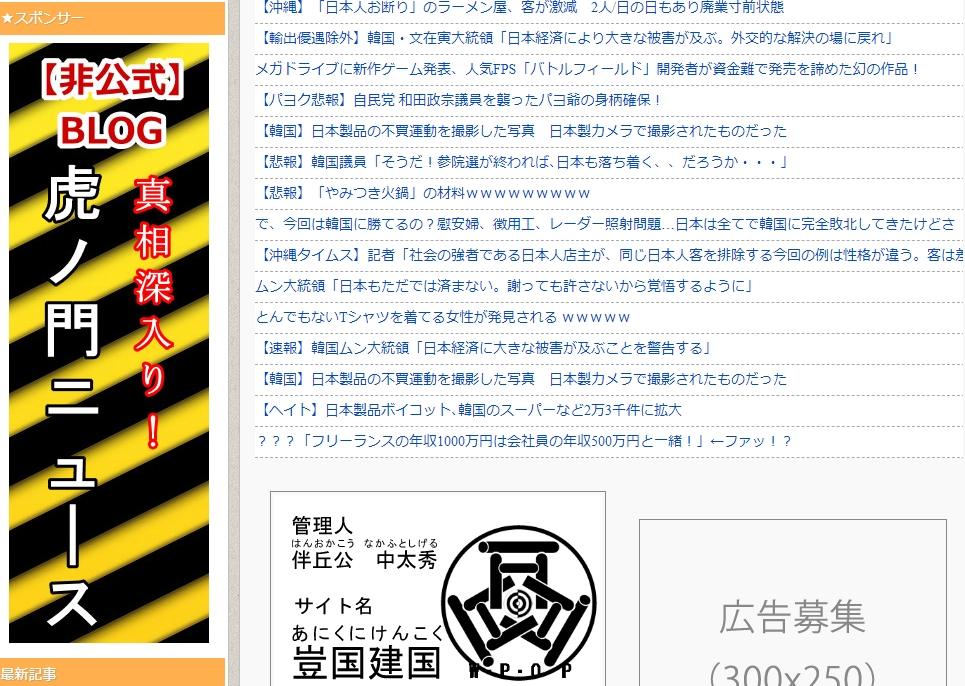
\includegraphics[width=\textwidth]{images/2channel/hoshusokuho.jpg}
  \caption{\textit{hoshu sokuhō} on 15-07-2019. (Screenshot by author. Source: hosyusokuhou.jp)}
  \label{fig:hoshusokuho}
 \end{subfigure}
  \begin{subfigure}[b]{0.45\textwidth}
  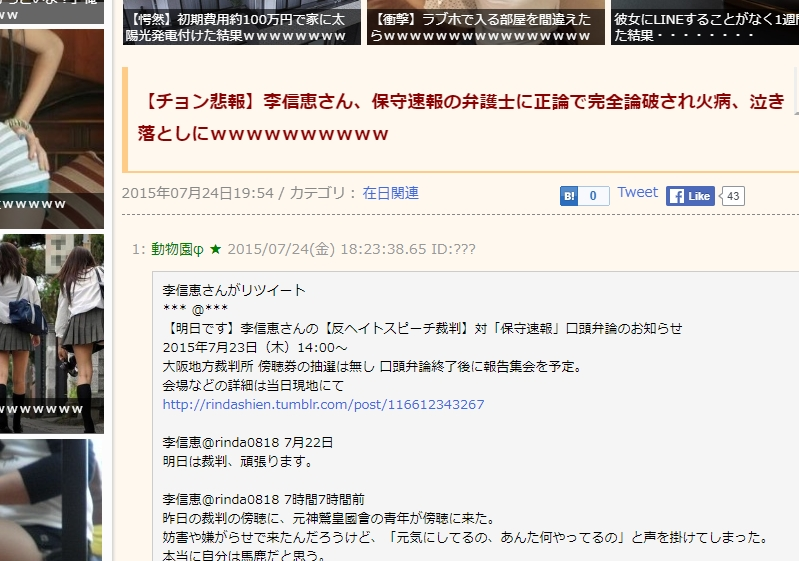
\includegraphics[width=\textwidth]{images/2channel/moeruasia.jpg}
  \caption{Moeruasia on 07-07-2016. (Screenshot by author. Source: moeruasia.net using archiving service archive.is)}
  \label{fig:moeruasia}
 \end{subfigure}
 \caption{Screenshots of 2channel-based \textit{matome} blogs}\label{fig:matome-examples}
\end{figure}

Disregarding the content of the aggregated items in \textbf{figure
\ref{fig:matome-examples}} (it should by now not be particularly
surprising that most items are related to Korean topics or left-wing
politics, often accompanied with the rhetorical device of '\emph{w}'s
for intended ridicule), two other things are of note. On \textbf{figure
\ref{fig:moeruasia}}, \emph{Moeruasia} uses the ethnic slur \emph{chon}
チョン as well as \emph{hibyō} / \emph{hwabyeong} (火病, a term
referring to a culture-bound mental illness). In the wake of this trial,
such \emph{matome} blogs have out precaution since opted to exclude
messages with explicit racial hatred from their aggregated posts.

\begin{quote}
「【チョン悲報】李信恵さん、保守速報の弁護士に正論で完全論破され火病、泣き落としにwwwwwwwwww」
\end{quote}

\begin{quote}
\emph{{[}Chon hihō{]} Ri Shine-san, hoshu sokuhō no bengoshi ni seiron
de kanzen ronpa sare kabyō, naki otoshi ni wwwwwwwwww}
\end{quote}

\begin{quote}
{[}Tragic \emph{Chon} News{]} Lee Sinhae was completely refuted by the
sound reasoning of Hoshu Sokuho's lawyer; falls into mental illness and
breaks down in tears \emph{wwwwwwwwww}
\end{quote}

The second point of note is on the screenshot of \emph{hoshu sokuhō}
(see \textbf{figure \ref{fig:hoshusokuho}}). As of July, 15 2019
\emph{hoshu sokuhō} is still in search of adverts. Whereas this blog had
previously been supported by ads of large companies as Epson (Hatachi
\protect\hyperlink{ref-hatachi__2018}{2018}), only one advertisement is
filled out (with a reference to a small-scale web-comic). To the left is
an advertisement for an unofficial fan-blog of Toranomon News
(\emph{toranomon nyūsu}, 虎ノ門ニュース).\footnote{This name most likely
  refers to the December 27, 1923 Toranomon incident (\emph{toranomon
  jiken}, 虎ノ門事件), an assassination attempt of the then Prince
  Regent Hirohito, committed under influence of left-wing ideologies.}
Although there is no substantial link between \emph{hoshu sokuhō} and
Toranomon News aside from a mutual target audience, I find that as a
conservative web-show drawing up to a combined half a million viewers
within its first day on YouTube and Niconico, Toranomon News is worth
briefly expanding upon for both its eclectic cast of ultra-right
conservative regular speakers as well as for its plethora of guest
speakers (see \textbf{figure \ref{fig:toranomon}}).

Sponsored by DHC Television,\footnote{Another show of DHC Television,
  News Girl (``\emph{Nyūsu joshi}'', 『ニュース女子』), gained criticism
  for its libelous reporting of a protest march in Okinawa in January
  2017, claiming that the demonstrators looked like terrorists, were
  being bribed, blocked ambulances and had (ethnic) Koreans amongst them
  (SANKEI DIGITAL INC
  \protect\hyperlink{ref-sankei_digital_inc_eng._2017}{2017}). Its panel
  and guest list overlaps with that of Toranomon News, and includes
  various celebrities and idols.} the majority of Toranomon News' hosts,
including Kent Gilbert and the Chinese born Seki Hei (Shi Ping), have
previously capitalized and continue to do so on a print-medium market
for historical revisionist and nationalist `Japan as Number One'
literature and literature highly critical of China and South
Korea.\footnote{Although there is a market for counter-argumentative
  literature as well. On 2019-4-6 a book with the following eye-catching
  title was published in Martin Fackler's name, the journalist with whom
  this paper opened: ``Precisely because I'm an American journalist is
  Japan's national disaster transparent'' (\emph{Beikoku hito
  jānarisutodakara minuketa Nihon no kokunan}
  『米国人ジャーナリストだから見抜けた日本の国難』 ). It's subtitle:
  ``The truth of this country that the media does not report''
  (\emph{media ga hontō no koto o tsutaenai kono kuni no shinjitsu}
  「メディアが本当のことを伝えないこの国の真実」).} Since 2015 they have
joined hands to influence public opinion and target the market for
nationalist rhetoric online, with YouTuber and imperial descendant
Takeda Tsuneyasu on the panel and YouTuber Kazuya as frequent guest (the
latter seen amongst the top Niconico videos back in chapter two in
\textbf{figure \ref{fig:nicotop}}). Other guests include Abe Shinzō
himself,\footnote{As Arimoto Kaori herself describes in an article on
  \emph{Sankei Shimbun} tabloid \emph{Yūkanfuji} (夕刊フジ), On the
  2019-07-13 edition of the annual cherry blossom viewing party
  (\emph{sakura o mirukai} 「桜を見る会」), Abe Shinzō was again seen in
  the company of various Toranomon News regulars including Arimoto
  Kaori, Hyakuta Naoki, Kent Gilbert, Takeda Kunihiko, Jōnen Tsukasa,
  Suda Shin'ichirō, Takeda Tsuneyasu, Fujii Genki and Ōtaka miki
  (Arimoto \protect\hyperlink{ref-arimoto_eng._2019}{2019}).} as well as
former Minister of Internal Affairs and Communications Yoshitaka Shindō,
various LDP lawmakers including Mio Sugita, \emph{Nippon Kaigi}
associate Sakurai Yoshiko and former idol Chiba Reiko.\footnote{Many of
  the above have contributed to the magazine Japanism as well. Volume 24
  'September 16, 2015), for example, includes writings by Kent Gilbert,
  Sugita Mio, Sakurai Makoto, Kurayama Mitsuru, while Volume 49 (June 8,
  2019) includes writings by Kazuya, Chiba Reiko and again Sugita Mio.}

\begin{figure}[!htb]
 \centering
 \begin{subfigure}[b]{0.5\textwidth}
  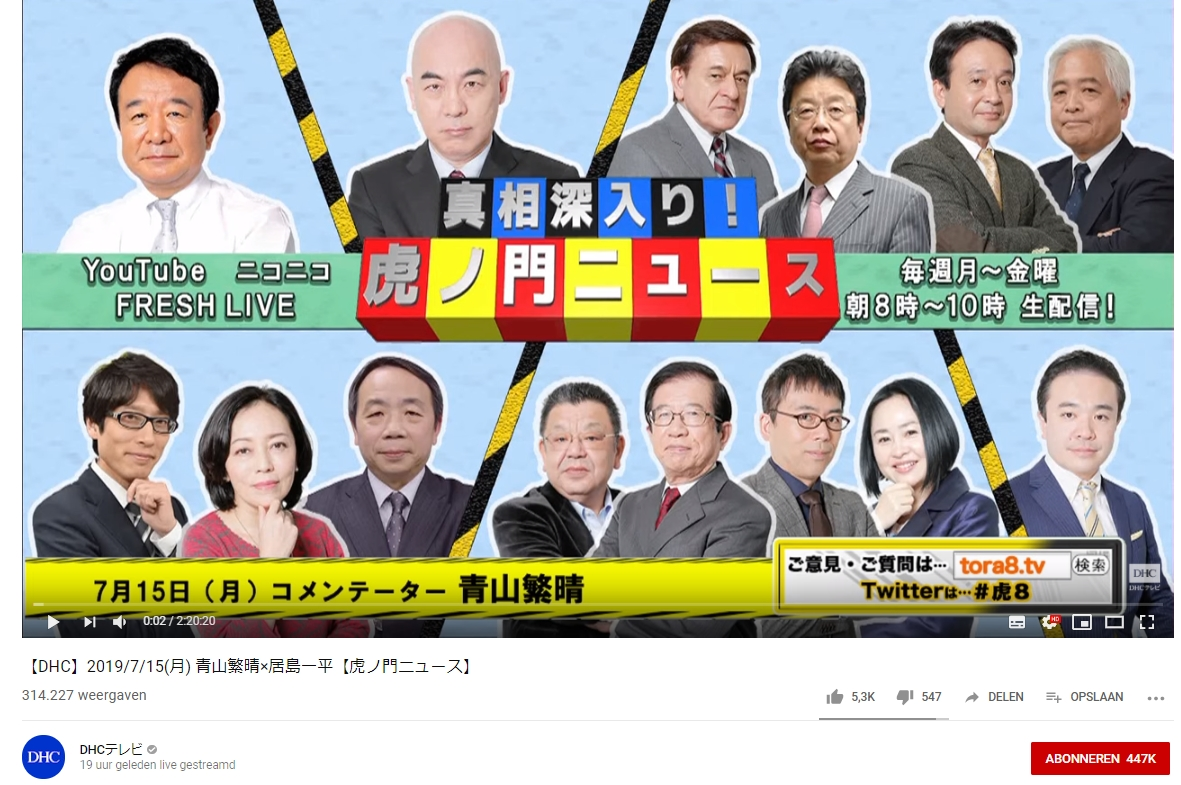
\includegraphics[width=\textwidth]{images/2channel/toranomon.jpg} 
  \captionsetup[sub]{font=scriptsize}
  \caption*{\textbf{Left to right}: Aoyama Shigeharu, Hyakuta Naoki, Kent Gilbert, Kitamura Haruo, Inoue Kazuhiko, Fujii Genki, Takeda Tsuneyasu, Arimoto Kaori, Seki Hei, Suda Shin'ichirō, Takeda Kunihiko, Jōnen Tsukasa, Ōtaka miki, Orishima Ippei (Screenshot by author. Source: YouTube.com)}
 \end{subfigure}
 \caption{Screenshot of Toranomon News on YouTube}\label{fig:toranomon}
\end{figure}

Hyakuta Naoki, regular commentator on Toranomon News and author of the
best-selling 2006 war drama ``The Eternal Zero'' (which in its 2013
screen-adaption won the Japan Academy Prize for best film) went on to
co-author 『日本よ、世界の真ん中で咲き誇れ』 (\emph{nihon yo, sekai no
man'naka de sakihokore}, ``Japan! Be Proud of Yourself in the Center of
the World!'') with Abe Shinzō in 2013 and was appointed by the latter as
board of governor member of Japan's national broadcast service NHK in
2013.\footnote{Abe gained further criticism with his appointment of
  ``comfort women'' apologist Katsuto Momii as chairman of NHK, in what
  the \emph{Japan Times} described as a ``trend toward self-censorship''
  (Sieg \protect\hyperlink{ref-sieg_under_2015}{2015}).} Although his
November 2018 bestseller \emph{Nihon Kokuki} (日本国紀, `Chronicle of
Japan') was criticized for historical revisionism and plagiarism from
Wikipedia (Yamamoto \protect\hyperlink{ref-yamamoto__2018}{2018}), he
subsequently followed up with the March 2019 『今こそ、韓国に謝ろう
~そして、「さらば」と言おう~』 (\emph{Ima koso, Kankoku ni ayamarō
\textasciitilde{} soshite,`saraba' to iō \textasciitilde{}}, ``Then let
us now apologize to Korea-and say, `Farewell'\,'').

Takeda Tsuneyasu is not without controversy either, posting, for
example, the following Tweet on May 22, 2016, enforcing stereotypes of
violent crimes linked to foreigners (Takeda
\protect\hyperlink{ref-takeda_eng._2016}{2016}):

\begin{quote}
「小金井ライブハウス殺人未遂事件で逮捕された人物は「自称・岩埼友宏容疑者」と報道されている。自称ということは本名でないということ。なぜ本名で報道しない?ここが日本のメディアのおかしいところ。臆する必要はない。本名で報道すべき。これは私の憶測だが、容疑者は日本国籍ではないと思われる。」
\end{quote}

\begin{quote}
``\emph{Koganei raibuhausu satsujin misui jiken de taiho sa reta
jinbutsu wa `jishō iwa saiyū Hiroshi yōgi-sha' to hōdō sa rete iru.
Jishō to iu koto wa honmyōdenai to iu koto. Naze honmyō de hōdō shinai?
Koko ga Nihon no media no okashī tokoro. Okusuru hitsuyō wanai. Honmyō
de hōdō subeki. Kore wa watashi no okusokudaga, yōgi-sha wa Nihon
kokusekide wa nai to omowa reru.}''
\end{quote}

\begin{quote}
``The person arrested for the Koganei Live House murder attempt is
reported as the `self-proclaimed' Tomohiro Iwasaki. `Self-proclaimed'
means it is not a real name. Why not report their real name? This is
strange of the Japanese media. There is no need to be hesitant. The
media should report it under their real name. This is my speculation,
but the suspect seems not to be of Japanese nationality.''
\end{quote}

\begin{figure}[!htb]
 \centering
 \begin{subfigure}[b]{1\textwidth}
  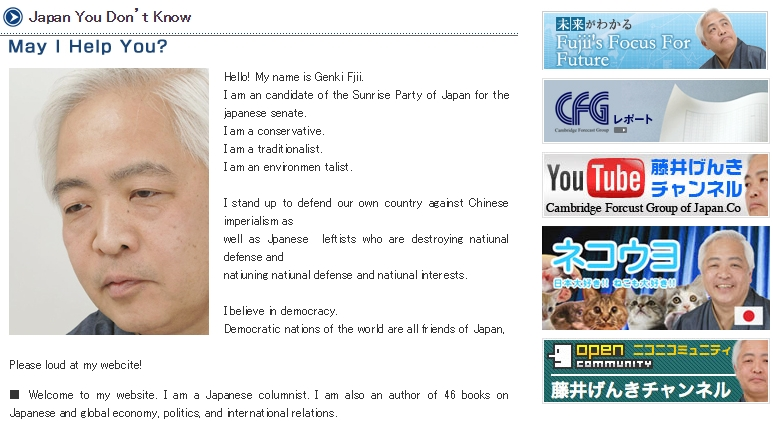
\includegraphics[width=\textwidth]{images/genkifuji.jpg}
  \caption*{(Screenshot by author. Source: gemki-fujii.com/english/)}
 \end{subfigure}
 \caption{Screenshot of Fuji Genki's English homepage (14-07-2019)}\label{fig:genkifuji}
\end{figure}

Some have embraced the Netto-Uyoku phrasing, such as YouTuber Fuji Genki
(see \textbf{Figure \ref{fig:genkifuji}}), who with 14,900 subscribers
on his main account has published videos both in English and Japanese on
accounts as Yamatotube2, \emph{Chan'neru kura-ra} チャンネルくらら and
\emph{hoshu ronkaku chan'neru+} 保守論客チャンネル+ (lit. `Conservative
Polemicist Channel+'). A conservative online voice, he has referred to
himself tongue-in-cheek as \emph{nekouyo} ネコウヨ (a wordplay literally
meaning `cat-right' as opposite to `net-right'). Of note is the English
language antagonizing both Chinese imperialists and Japanese leftists as
anti-Japanese elements, and the literal translation ``Japan You Don't
Know'' (most likely from the common rhetorical device \emph{anata no
shiranai nihon} 「あなたの知らない日本」), implying a \emph{real} Japan
hidden by the mainstream press.

\section[Wikipedia]{\texorpdfstring{Wikipedia\footnote{Throughout this
  section, I will refer to Wikipedia users using single quotation marks
  (with additional \emph{romanized} readings when required). When I
  translate Wikipedia articles I use italics and single quotation marks,
  adding the romanized readings and original Japanese expression the
  first I time refer to that article.}}{Wikipedia}}\label{wikipedia76}

Whereas the software the Japanese 2channel and English 4chan are based
on were influential in shaping online communities throughout the late
90s and early `00s, the software Wikipedia (a free online encyclopedia
based on transparent and open collaboration) runs on, MediaWiki, has
since its inception in 2002 gained much traction worldwide. Uses range
from the political realm\footnote{Governmental instances in the United
  States use the software as a content management system for internal
  information sharing (Diplopedia and Intellipedia), for example.
  WikiLeaks, famous for publishing various sensitive documents, was
  originally built on this software as well.} to lighter
topics,\footnote{Wikipedia co-founder Jimmy Wales founded \emph{Fandom},
  a for-profit variant of MediaWiki, specifically for in-depth pages on
  popular culture topics.} and Wiki-style sub-communities are build
around every possible aspect of popular culture.\footnote{I have for
  example found numerous Japanese Wiki-style outlets solely on the topic
  of AKB48's idol formations, with \url{https://48pedia.org} (as of
  12-07-2019) alone already containing 2,062 pages.} Wikipedia itself is
as of 2019 the \nth{5} most visited website in the world and \nth{6}
most in Japan; with 7 percent of all articles being written in Japanese
(the \nth{2} most represented language on Wikipedia). The specific
mannerisms of utilizing Wikipedia have formed distinct subcultures and
group dynamics, and vandalism or so-called \emph{edit-wars} (disputes
over content through reverting and adjusting user contributions) are not
uncommon elements of those. The open nature of Wikipedia and its
underlying MediaWiki software permits us a glimpse into topics that
Wikipedia editors place high importance on. \textbf{Table
\ref{tab:50mostcont}},\footnote{This is a translation. For the
  methodology employed as well as the original, slightly more expanded
  list, I refer to section \ref{sec:wikiappendix} and \textbf{table
  \ref{tab:50expanded}} on page \pageref{tab:50expanded}.} for example,
displays the top fifty most 'contentious' articles on the Japanese
Wikipedia as of 2019 (in other words, articles that have high rates of
such \emph{edit-warring}, based on the amount of reverts done in
contrast to the total amount of edits).\footnote{As of 2019, the article
  with the highest rate of reverts in contrast to its rate of revisions
  is the topic of Japanese war crimes in Nanjing during the Second
  Sino-Japanese War. This paper follows the English designations as used
  by Wikipedia. \emph{Nankin jiken} 南京事件 is therefore not translated
  as Nanjing Incident but as Nanjing Massacre instead.}

\begin{table}[!htb]
\footnotesize
\centering
\setlength{\tabcolsep}{5pt}
\caption{50 most contentious articles on the Japanese Wikipedia (2019)}\label{tab:50mostcont}
\scalebox{0.8}{
\begin{tabular}{@{}p{0.1cm}lp{0.1cm}lp{0.1cm}lp{0.1cm}l@{}}
\toprule
1&Nanjing Massacre&14&Soka Gakkai&27&Keisuke Honda&40&HKT48\\
2&Netto Uyoku&15&Emperor&28&SKY PerfecTV! Channel List&41&South Korea\\
3&Japan&16&Taiwan&29&List of terms in ONE PIECE&42&Shuriken Sentai Ninninger\\
4&Maeda Atsuko (AKB48)&17&Mr. Osomatsu&30&List of monsters in Kamen Rider Series&43&Hatsune Miku\\
5&Shichibukai (One Piece)&18&Yuna Kim&31&K-on!&44&Witchy PreCure!\\
6&Devil's Fruit (One Piece)&19&Zaitokukai&32&Kantai Collectrion-Kancolle-&45&Fate / Grand Order\\
7&One Piece&20&Rino Sashihara (HKT48)&33&Navy (One Piece)&46&Magical Girl Madoka $\star$ Magica\\
8&Watanabe Mayu (AKB48)&21&Zainichi Koreans in Japan&34&Takahashi Minami (AKB48)&47&Kimura Takuya (SMAP)\\
9&Nogizaka46&22&Sakurai Sho (Arashi)&35&Kamen Rider Ghost&48&Naruto Characters\\
10&AKB48&23&Akihito&36&Hitoshi Matsumoto&49&Minecraft\\
11&Abe Shinzo&24&YouTube&37&Doubutsu Sentai Zyuohger&50&Korea origin theory\\
12&Keyakizaka46&25&Monkey D. Luffy (One Piece)&38&DPR Korea\\
13&Yukio Hatoyama&26&Asahi Shimbun&39&Hiroiki Ariyoshi\\
\bottomrule
\end{tabular}
}
\end{table}

Based on these statistics, I find that regardless whether sorted by
total revisions, total reverts or total `contention', the lists of
Wikipedia articles are dominated almost entirely with articles devoted
to Japanese idol pop-artists (in particular AKB48) and animation
(specifically One Piece). Sorted on either total reverts or total
contention these lists include throughout the years topics such as Abe
Shinzo, Japan, Sōka Gakkai, the Nanjing Massacre, Netto-Uyoku, both
South and North Korea, and Zainichi Koreans. Throughout other years,
this list has included topics such as the South Korean figure skater
Yuna Kim,\footnote{In the wake of Yuna Kim's victory over the Japanese
  skater Mao Asada during the 2010 Winter Olympics, rumors were spread
  on \emph{2channel} over a supposed improper win (CNN
  \protect\hyperlink{ref-cnn_korean_2010}{2010}).} the topic of male
discrimination (\emph{dansei sabetsu} 男性差別), an article on a
supposed \emph{Korean origin theory} (\emph{kankoku kigen-setsu}
韓国起源説), global warming, Ishihara Shintarō, Hashimoto Tōru and the
former Prime Ministers Asō Tarō, Hatoyama Yukio, Kan Naoto and Koizumi
Jun'ichirō.

Of immediate note is 1. the position of Netto-Uyoku as \nth{2} most
contentious article (already implying that Netto-Uyoku are highly active
on Wikipedia), and 2. a seemingly distinct lack of articles that would
otherwise be considered controversial topics, such as the territorial
disputes of the Liancourt Rocks. These are however missing primarily due
administrators' ability to `protect' articles from anonymous edits (or
even any edit in general) until new information comes up. That being
said, on a platform that is dominated by articles on pop-culture when
viewed over large time lapses, a closer look at top edits per month does
reflect topical events. As that particular dispute gained renewed
traction, so did the Japanese article on the Liancourt Rocks, for
example, reach first spot as the most edited article of August 2012.
Moreover, so did between May and June 2006 various other articles
related to Netto-Uyoku sentiment reach first or otherwise high
spots.\footnote{in order the following articles all reached top
  revisions for those months: `\emph{Anti-Korean sentiment}'
  (\emph{kenkan}, 嫌韓), `\emph{Zchannel}' (2ちゃんねる), `\emph{South
  Korea}' (\emph{daikanminkoku}, 大韓民国), `\emph{The Women's
  International War Crimes Tribunal on Japan's Military Sexual Slavery}'
  (\emph{josei kokusai senpan hōtei}, 女性国際戦犯法廷),
  `\emph{Japan--Korea disputes}' (\emph{nikkanmondai}, 日韓問題),
  `\emph{minority discrimination}' (\emph{minzoku sabetsu}, 民族差別),
  `\emph{Anti-Japanese Sentiment}' (\emph{han'nichi}, 反日),
  `\emph{ishihara shintarō}' (石原慎太郎), `\emph{Right of foreigners to
  vote}' (\emph{gaikokuninjinseiken}, 外国人参政権), `\emph{Special
  Privileges of the Zainichi}' (\emph{zainichi tokken}, 在日特権).}

During the early 2000s when articles on common topics were still being
written from the ground up, reverts were uncommon to the point that they
are not a reliable way to express quantifiable controversy in this time.
Based on the total amount of revisions as an indicator of perceived
importance by the Japanese Wikipedia community, top articles in the
early days of the Japanese Wikipedia contain however few articles
related to such pop culture phenomena. Instead in 2003 the most revised
articles include the topics of the Japanese railway,\footnote{Such as
  \emph{`List of railway stations in Japan'} (\emph{nihon no tetsudō-eki
  ichiran}, 日本の鉄道駅一覧), \emph{`List of railway lines in Japan'}
  (\emph{nihon no tetsudō rosen ichiran}, 日本の鉄道路線一覧),
  \emph{`Tokyo Express Railway'} (\emph{tōkyōkyūkōdentetsu},
  東京急行電鉄) and \emph{`Japanese National Railway 113-series Trains'}
  (\emph{kokutetsu 113-kei densha}, 国鉄113系電車). High interest in
  railways and trains (\emph{tetsudō otaku} 鉄道オタク or \emph{densha
  otaku} 電車オタク) is not an uncommon phenomenon.} religion\footnote{\emph{`Christian
  glossary'} (\emph{kirisutokyō yōgo ichiran} キリスト教用語一覧),
  \emph{Catholicism} (\emph{katorishizumu}, カトリシズム),
  \emph{`Christianity'} (\emph{kirisutokyō}, キリスト教), \emph{`List of
  Gods'} (\emph{kami no ichiran}, 神の一覧) and \emph{`Religion'}
  (\emph{shūkyō}, 宗教)} as well as topics related to China\footnote{\emph{`China'}
  (\emph{chūgoku}, 中国), \emph{`Taiwan'} (台湾), \emph{`List of Chinese
  Emperors' } (\emph{chūgoku teiō ichiran}, 中国帝王一覧)} and Japanese
history.\footnote{\emph{`World War II'} (\emph{dainijisekaitaisen},
  第二次世界大戦), \emph{`Pacific War'} (\emph{taiheiyōsensō},
  太平洋戦争), \emph{`Japanese History'} (\emph{nihon'norekishi},
  日本の歴史)} In 2004 2channel joins the top of this list as second
most revised article, alongside articles related to
media-channels\footnote{\emph{`Fuji Television'} (\emph{Fuji terebijon},
  フジテレビジョン), \emph{`Nippon Television Broadcasting Network'}
  (\emph{nihon terebi hōsōmō}, 日本テレビ放送網), \emph{`TV TOKYO'}
  (\emph{terebi tōkyō}, テレビ東京), Mainichi Broadcasting
  (\emph{mainichi hōsō}, 毎日放送), \emph{`Tokyo Broadcasting Holdings'}
  (\emph{tōkyōhōsō hōrudingusu}, 東京放送ホールディングス), \emph{`Japan
  Broadcasting Association'} (\emph{nihon hōsō kyōkai}, 日本放送協会),
  \emph{`Chubu Nippon Broadcasting'} (\emph{chūbu nippon hōsō},
  中部日本放送), \emph{`Nippon Broadcasting'} (\emph{nippon hōsō},
  ニッポン放送), \emph{`Asahi Broadcasting Group Holdings'}
  (\emph{asahihōsō gurūpu hōrudingusu} 朝日放送グループホールディングス)}
and the Korean peninsula. It is only from 2005 onwards that we perceive
an increase of mass-edited articles on pop-media (animation as
\emph{crayon shin-chan} クレヨンしんちゃん, \emph{doraemon} ドラえもん,
One Piece and Naruto reach the top of this list). Although this rate has
decreased over the years, the rate of anonymous edits on the Japanese
Wikipedia is still remarkably high when contrasted to the global scale;
an indication of 2channel's \emph{modus operandi} seeping into Wikipedia
(see \textbf{figure \ref{fig:anon-wiki}}). Although anonymity is to be
taken with a grain of salt, considering IP addresses are publicly
available, of note here is particularly the intent of the user not to be
associated with a user-name.

\begin{figure}[!htb]
 \centering
 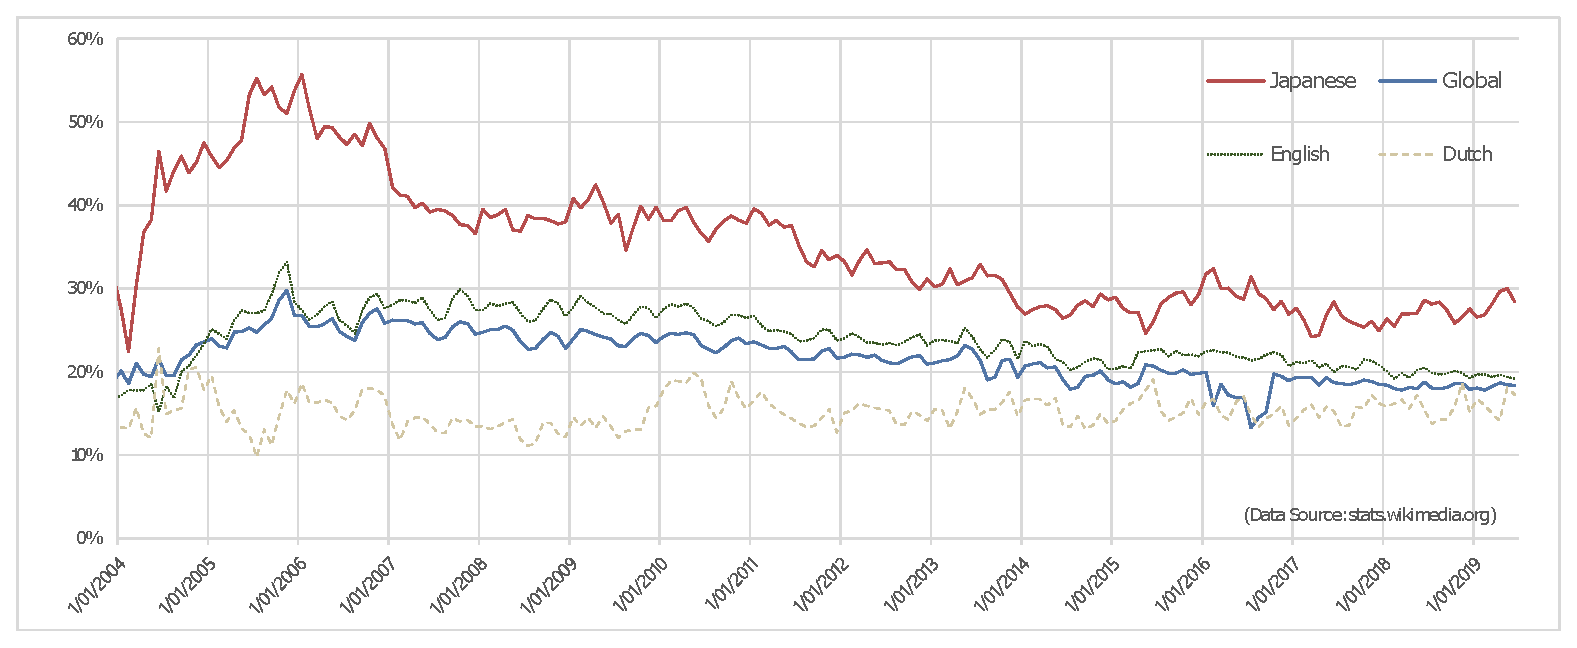
\includegraphics[width=0.95\textwidth,trim=4 4 4 4,clip]{images/anon-wiki.eps}
 \centering\caption{Percentage of Anonymous Edits in Japanese and Worldwide (15 Years)}\label{fig:anon-wiki}
\end{figure}

Using the statistic tool-set \emph{XTools},\footnote{An open-source
  tool-set building on the Wiki-media API, available at
  \url{https://www.mediawiki.org/wiki/XTools}.} one gets further
insights into the revision history of each article, as well as into the
Wikipedia users contributing to them. An overview of revision statistics
on two contested topics (see \textbf{figures \ref{fig:xtools-zainichi}
and \ref{fig:xtools-asahi}}) shows a sharp increase of activity in the
period of 2009-11, an increase that cannot be explained solely by a rise
in usage of Wikipedia as a platform but falls in line with the
aforementioned increase of interest in right-wing politics
(\textbf{figure \ref{fig:politictrends}}) and Netto-Uyoku
(\textbf{figure \ref{fig:nettouyoku}}). This is confirmed by the
relative word count to the amount of edits, which is aside, aside from
the 2011 peak in edits of \textbf{figures \ref{fig:xtools-zainichi}},
not in proportion and indicates again the contentious character of the
topic on Wikipedia.

\begin{figure}[!htb]
 \centering
 \begin{subfigure}[b]{0.49\textwidth}
  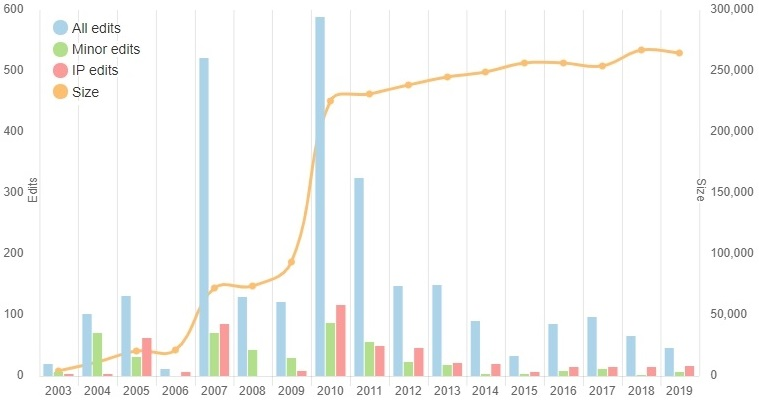
\includegraphics[width=\textwidth]{images/wiki/zainichi.jpg}
  \caption{\textit{'Zainichi Koreans'} (Source: xtools.wmflabs.org)}
  \label{fig:xtools-zainichi}
 \end{subfigure}
  \begin{subfigure}[b]{0.49\textwidth}
  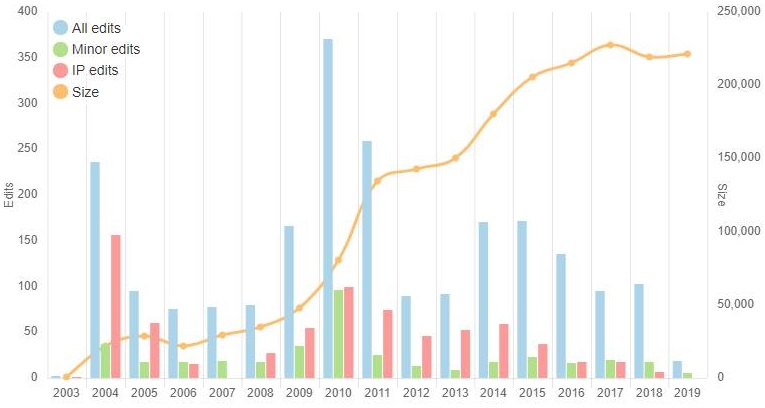
\includegraphics[width=\textwidth]{images/wiki/asahi-shimbun.jpg}
  \caption{\textit{'Asahi Shimbun'} (Source: xtools.wmflabs.org)}
  \label{fig:xtools-asahi}
 \end{subfigure}
 \caption{Revision Statistics for Japanese Wikipedia Article \textit{'Zainichi Koreans'} and \textit{'Asahi Shimbun'}}\label{fig:xtools}
\end{figure}

The article on Netto-Uyoku then has seen 2,281 edits by 756 users since
its creation on September 30, 2005 with an anonymous revision:

\begin{quote}
「ネット上で徘徊・跋扈する馬鹿な右翼のこと。2ちゃんねるなど無責任な管理者が運営する掲示板に生息する。また、まじめな議論をおこなおうとする、右翼に批判的な掲示板などを荒らすことも生業としている。2ちゃんねる風のプラカードをもって、杉並で「つくる会」教科書採択のために策動した連中もいる。」
\end{quote}

\begin{quote}
``\emph{Netto-jō de haikai bakko suru bakana uyoku no koto. 2-Chan neru
nado musekinin'na kanrisha ga un'ei suru keijiban ni seisoku suru. Mata,
majimena giron o okonaou to suru, uyoku ni hihantekina keijiban nado o
arasu koto mo nariwai to shite iru. 2-Chan neru kaze no purakādo o
motte, Suginami de `tsukurukai' kyōkasho saitaku no tame ni sakudō shita
renchū mo iru.}''
\end{quote}

\begin{quote}
``Stupid right-wingers loitering on the Internet. They inhabit bulletin
board systems (BBS) such as 2channel, operated by irresponsible
administrators. Moreover, they call for trolling Bulletin Board Systems
meant for attempting serious discussion and/or for making critical
arguments against the right. There are also those that have participated
in the Suginawa protests on the adoption of a new school textbook with
2channel-themed placards.''\footnote{This refers to an event in 2005,
  \emph{Suginami-ku rekishi kyōkasho saitaku sōdō}
  (杉並区歴史教科書採択騒動, ``Suginami Ward history textbook adoption
  riot'') wherein groups both agreeing with and protesting the adoption
  of a new history schoolbook for public education (which would lessen
  the focus on topics deemed masochistic) took to the Suginawa Ward in
  Tokyo for public protest. \emph{2channel} users in particular
  protested supposed ties of protesters with the New Left (in particular
  the Revolutionary Communist League, National Committee or Chūkaku-ha).}
\end{quote}

Since then the article has grown to contain 70,744 characters and is
linked to from other pages 405 times, an indication of the term steadily
seeping into public discourse. As shown in \textbf{table
\ref{tab:50mostcont}}, the topic remains controversial amongst certain
users. The very last edits in my data-source (and thus the most recent
at July 2, 2019) are the following addition and its subsequent
revert:\footnote{A user whose further edits include the addition
  「日本人に経済保証と謝罪をした上で滅びるべき国家である。」
  (\emph{Nihonjin ni keizai hoshō to shazai o shita ue de horobirubeki
  kokkadearu}, lit. ``A nation that after giving economic guarantees and
  apologies to the Japanese people, ought to be destroyed''), to the
  Japanese article of `\emph{South Korea}' and some vandalism to the
  article of South Korean idol formation TWICE. Edits to that article
  include amongst others changing Japanese member 名井 南 (Myōi Mina) to
  \emph{han-nichi, baikoku-yatsu} (「反日、売国奴」, `anti-Japanese,
  traitorous bastard') and later \emph{uragirimono no nihonjin} (「
  裏切り者の日本人」, `traitorous Japanese').}

\begin{quote}
「日本を取り戻し、世界でもっとも輝ける国にするために日々研鑽を惜しまない素晴らしい方達である。そのために、日本人による正当な民族差別を率先して行っている。」
\end{quote}

\begin{quote}
``\emph{Nihon o torimodoshi, sekai de mottomo kagayakeru kuni ni suru
tame ni hibi kensan o oshimanai subarashīi kata-tachi dearu. Sono tame
ni, nihonjin ni yoru seitōna minzoku sabetsu o sossen shite itte iru.}''
\end{quote}

\begin{quote}
``These are wonderful people who do not spare time in order to restore
Japan and making it the brightest country in the world. To that end,
they takes the initiative of legitimating ethnic discrimination by
Japanese people.''
\end{quote}

Here, the phrasing of `restoring Japan' is eerily similar to prime
minister Abe's political catch-phrase `We will restore Japan'
(\emph{nippon o torimodosu} 「日本を、取り戻す。」), used during his
political campaign against the DPJ in the wake of the 2011 earthquake.
As is what I translated as `brightest country' similar to prime minister
Abe's 『美しい国へ』 (\emph{Utsukushii kuni he} `Toward a Beautiful
Nation'). The initially vague expressions of `restoring' (from what?)
and `bright' or `beautiful' country (defined how?) are implicitly
answered by this user: normalization of ethnic discrimination is a means
to restore Japan (from ethnic minorities) and make it a bright
(ethnically homogeneous) country.

A constant in these contested pages are large contributions by a small
group of people. The top contributor to the article of \emph{Nanking
Massacre} (27.7\% of all edits, between the period of November 1, 2009
and April 16, 2019), for example, is a user by the handle of
\emph{yamato-yashiki} (大和屋敷). This is a user with as of July 2, 2019
16,682 edits over 3,229 pages including 139 edits to English Wikipedia
articles (where he has since been blocked from contributing, having
focused primarily on topics related to Korea, such as `Korean
Nationalism' and the `Japan-Korea Treaty of 1910', as well as `softer'
topics as \emph{otaku}, \emph{Yakiniku} and `Secret photography').
Moreover, this user is amongst the top editors (based on frequency of
personal edits compared to total edits) for other such contested topics
as \emph{Netto-Uyoku} (first place with 19.7\%). The second largest
contributor to this article (with 166 or 15.7\% edits between October
21, 2015 and March 17, 2019) is `Japanese Sincerity', which is a
twin-account of the since blocked account `Japanese spirits' (and most
likely a reference to \emph{yamato-damashii} 大和魂, a normative
expression of \emph{nihonjin}-style Japanese ethno-nationalism). A look
at the profile page of `Japanese Sincerity' on Wikipedia reveals the
following information:

\begin{quote}
「得意分野\newline
日本史(特に昭和の時代)。イデオロギーでなく、事実の正確な記述や広い視点による解釈に固執します。記述に恣意的に反映するかどうかは別として、個人的には日本の皇室の大ファンであり、それも昭和天皇、上皇、今上天皇と戦後皇室の在り方に個人的には共感しています。」
\end{quote}

\begin{quote}
``\emph{Tokui bun'ya\newline
nihonshi (tokuni Shōwa no jidai). Ideorogīdenaku, jijitsu no seikakuna
kijutsu ya hiroi shiten ni yoru kaishaku ni koshū shimasu. Kijutsu ni
shii-teki ni han'ei suru ka dō ka wa betsu to shite, kojin-teki ni wa
Nihon no kōshitsu no dai fandeari, sore mo shōwadenkō, jōkō, kinjōten'nō
to sengo kōshitsu no arikata ni kojin-teki ni wa kyōkan shite imasu.}''
\end{quote}

\begin{quote}
``Specialty\newline
Japanese history (in particular the Showa era). I am not ideological,
and instead stick to writing accurate, factual descriptions and
interpretations through broad perspectives. Regardless of whether it
reflects in my articles, I am a big fan of the Imperial House of Japan,
and feel sympathetic to the state of the Showa Emperor, Emperor Akihito,
Emperor Naruhito and the postwar imperial family.'' (source:
\url{https://ja.wikipedia.org/wiki/\%E5\%88\%A9\%E7\%94\%A8\%E8\%80\%85:Japanese_sincerity})
\end{quote}

\begin{figure}[!htb]
 \centering
 \begin{subfigure}[b]{1\textwidth}
  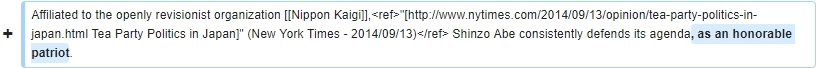
\includegraphics[width=.9\textwidth]{images/wiki/japanese-spirits-abe.jpg}
  \caption*{(Screenshot by author. Source: ja.wikipedia.org)}
  \label{fig:nicotop}
 \end{subfigure}
 \caption{English Wikipedia Edits by User 'Japanese spirits' on 'Shinzō Abe'}\label{fig:js-abe}
\end{figure}

Contrary to that statement, the topics of choice and their particular
edits do reveal an ideological point of view. Of note are this user's
455 contributions to the English language Wikipedia, as well as several
to the Spanish (46) and French Wikipedia (28), dominantly on topics of
Japanese war crimes. As shown in \textbf{\ref{fig:js-abe} and
\ref{fig:js-inada}}, through the now banned twin-account of `Japanese
spirits' this user has formerly contributed to English articles on Inada
Tomomi and Abe Shinzō with apologetic, reactionary edits (the former
which are as of July 9, 2019 still largely in-tact). Support for the
revisionist agenda of Nippon Kaigi is in this user's logic an act of
honor and patriotism. Criticism of the Yasukuni Shrine too is
disrespectful towards ``the souls of dead Japanese soldiers'' and,
furthermore, the 2017 critical documentary \emph{Yasukuni} betrayed a
Chinese tinted political agenda. Through their main account `Japanese
Sincerity', this user has since opted for a softer tone. Their last
contribution, on the article for `Pantingan River massacre' (which too
is still largely intact as of July 9, 2019), attempts to downplay events
with the following line:

\begin{quote}
``Following Tsuji's abnormal order which was considered to be a war
criminal and beyond his commission, Japanese 122 Regiment of Sixty-fifth
Brigade executed the US and Philippine soldiers in the Pantingan River
{[}2{]}. Colonel Takeo Imai, of another Japanese regiment, was doubt the
authority of the order which came from the top but not clearly from who?
and Imai ignored the cruel order and did not any execusion{[}3{]}
(\emph{sic}).''
\end{quote}

\begin{figure}[!htb]
 \centering
 \begin{subfigure}[b]{0.9\textwidth}
  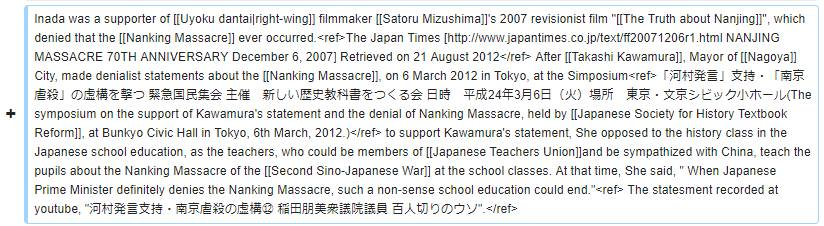
\includegraphics[width=\textwidth]{images/wiki/japanese-spirits-inada1.jpg}
 \end{subfigure}
 \begin{subfigure}[b]{0.9\textwidth}
  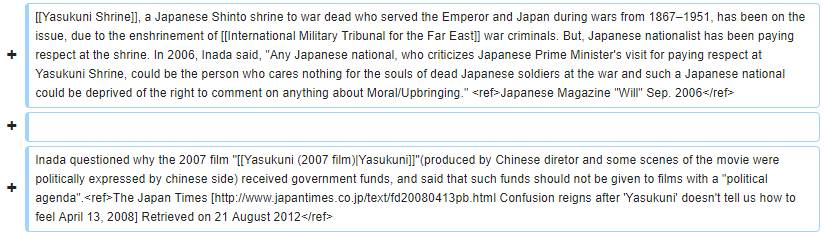
\includegraphics[width=\textwidth]{images/wiki/japanese-spirits-inada2.jpg}
 \end{subfigure}
 \begin{subfigure}[b]{0.9\textwidth}
  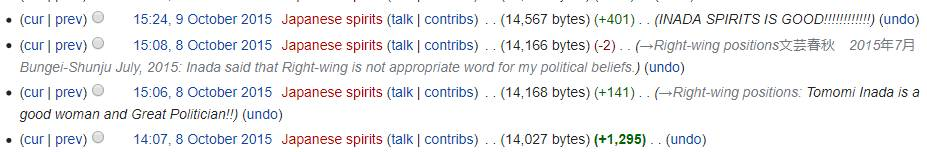
\includegraphics[width=\textwidth]{images/wiki/japanese-spirits-inada0.jpg}
  \caption*{(Screenshot by author. Source: ja.wikipedia.org)}
 \end{subfigure}
 \caption{English Wikipedia Edits by User 'Japanese spirits' on 'Tomomi Inada'}\label{fig:js-inada}
\end{figure}

Another prolific Wikipedia user (and contributor to the \emph{Nanking
Massacre} article with 10.5\% of its edits done between December 3, 2009
and April 30, 2019) is the user `\emph{kachō fūgetsu setsugetsuka
keibu}' (`花蝶風月雪月花警部').\footnote{The origin of the name is
  unclear but possibly refers to a poem. 花蝶風月 \emph{kachō fūgetsu}
  is the title of a popular \emph{vocaloid} composition \emph{dōjin}
  album released on Comiket in 2017, and translates as ``Beauty of
  Flowers and Butterflies'' or ``Blossoms and butterflies, the cool
  breeze and a bright moon.'' 雪月花 \emph{setsu gekka} refers to an
  ancient Chinese poem (attributed to Bai Juyi) and is a common theme
  amongst ukiyo-e artists. It translates as ``Snow, Moon and Flowers.''
  警部 \emph{keibu} translates as ``police force'' and possible refers
  to the user's role as an administrator or supervisor on Wikipedia.}
The actions of this user however involve policing primarily un-sourced
or biased edits, and an online search of this account reveals several
topics accusing that user of being an `Anti-Japanese leftist traitor'
(\emph{han-nichi baikoku sayoku} 反日売国サヨク) and an ethnic Korean
(\emph{zainichi chōsenjin} 在日朝鮮人).\footnote{See for example
  \url{https://detail.chiebukuro.yahoo.co.jp/qa/question_detail/q10183667130}
  and
  \url{https://detail.chiebukuro.yahoo.co.jp/qa/question_detail/q13171578898}.}
One other such active user, `JapaneseA' (2,655 pages created and 46,343
pages edited) has received similar critique.\footnote{See for example
  \url{https://detail.chiebukuro.yahoo.co.jp/qa/question_detail/q10171294600}.}
Their policing conflicts have led to bans of active editors such as
`Chichiii', who has added 11,999 edits to 3,926 articles and authored
572 articles including \emph{Emperor Apologize request by Korea}
(\emph{Kankoku ni yoru ten'nō shazai yōkyū} 韓国による天皇謝罪要求),
\emph{Foreign Regional Suffrage} (\emph{gaikokujin chihō sansei-ken}
外国人地方参政権) and \emph{The issue of the Chinese Embassy and Primary
land acquisition in Tokyo} (\emph{chūgoku taishikan tonai ittōchi baishū
mondai} 中国大使館都内一等地買収問題).\footnote{A MediaWiki-based
  \emph{2channel} aggregation (\emph{matome}) page,
  2ちゃんねるウィキペディアスレまとめwiki (\emph{2-channeru wikipedia
  sure matome wikki}, `2channel Wikipedia tread aggregation Wiki')
  contains entries on various of the aforementioned Wikipedia editors.
  The entry on `Chichiii' in particular states ``Joined with an account
  in 2008. A typical neto-uyo, this user happily writes revisions
  whenever Zainichi Koreans have cause some kind of incident''
  (\emph{``2008-Nen kara akaunto de sanka. Tenkei-tekina neto-uyodeari,
  zainichichōsenjin ga nanika jiken o okosu to ōyorokobi de kahitsu
  suru''},
  「2008年からアカウントで参加。典型的なネトウヨであり、在日朝鮮人が何か事件を起こすと大喜びで加筆する」).
  For more information, see
  \url{https://jawp2ch.miraheze.org/wiki/Chichiii}.}

If we take a look at some of the other contested articles, similar
trends arise. Going through the revision history of articles as
\emph{`Japan'} (\emph{`nihon'}, 日本), \emph{`Hatoyama Yukio'}
(鳩山由紀夫), \emph{`Foreign suffrage in Japan'} (\emph{nihon ni okeru
gaikokujin sanseiken}, 日本における外国人参政権), \emph{`Zainichi
Koreans'} (\emph{zainichi kankoku・chōsenjin} 在日韓国・朝鮮人),
\emph{`Asahi Shimbun'} (朝日新聞) and \emph{`Zaitokukai'} reveals
primarily edits by `Chichiii', \emph{`kachō fūgetsu setsugetsuka keibu'}
(`花蝶風月雪月花警部' and `\emph{yamato yashiki}'
(`大和屋敷').\footnote{Going through the article on \emph{Zaitokukai} in
  particular reveals a large portion of blocked accounts, including for
  example contributor \emph{Asahara Shoko} 麻原彰晃, a reference to Aum
  Shinrikyo founder Asahara Shoko.} Another top contributor with a
telling user name to that latter article is the user \emph{`takeshima wa
nihon'} (`竹島は日本', translated as `Takeshima is Japanese'), who has
also contributed to articles related to 2channel,\footnote{In particular
  the topics \emph{`2channeler'} (\emph{2-channerā}, 2ちゃんねらー),
  \emph{`List of \emph{2channel} boards'} (\emph{2-channeru no ita no
  ichiran}, 2ちゃんねるの板の一覧) and `\emph{news bulletin (VIP) +
  board}' (\emph{nyūsu sokuhō (VIP) + ita}, ニュース速報(VIP)+板).}
Baseball star Suzuki Ichirō (popularly referred to as \emph{Ichirō},
イチロー) and the Wikipedia article on Makoto Sakurai.

One aspect of personalization on Wikipedia is the usage of badges on
one's profile.\footnote{For a full list of such badges, see
  \url{https://ja.wikipedia.org/wiki/Wikipedia:\%E3\%83\%A6\%E3\%83\%BC\%E3\%82\%B6\%E3\%83\%BC\%E3\%83\%9C\%E3\%83\%83\%E3\%82\%AF\%E3\%82\%B9}.}
Take, for example, user `S.S.Exp.Hashimoto'; a user primarily active on
railway-related articles but just as well a top contributor to the
articles \emph{`Netto-Uyoku'}, \emph{`Taiwan'} and \emph{`Foreign
suffrage in Japan'} (with a total of 4,698 pages edited between February
28, 2004 and July 6, 2019, including several on the English Wikipedia).
The user-page includes some information on the user's interest in
railways (the handle itself is a reference to the Keio Line semi-express
train towards Hashimoto, Kanagawa prefecture) and 2channel. More
interesting is however this user's usage of badges, as illustrated on
\textbf{figure \ref{fig:hashimoto}}. Badges that should be pointed out
are not uncommon, as seen on the profile of a top contributor to the
article on \emph{`asahi shimbun'}, user \emph{`gokoku bōkyō-dan'}
(`護国防共団', lit. `anti-communist national defense corps') and article
\emph{Taiwan} top editor `Kamakura' (who between August 19, 2003 and
June 30, 2019 had made 7,616 edits to over 3,933 articles, including 315
edits on the English wikipedia). This is illustrated on respectively
\textbf{figure \ref{fig:defense-corps}} and \textbf{figure
\ref{fig:kamakura}}.

In all three cases do the users express support for the Self Defense
Force (SDF). `S.S.Exp.Hashimoto' and `Kamakura' both take pride in their
identity as 2channel users,\footnote{The catchphrase used on that
  particular badge (「この利用者は2ちゃんねらーですが何か?」 \emph{Kono
  riyōsha wa 2-chan nera ̄ desugananika?}) translates as a rhetorical
  question expressing indifference, ``This user is a 2channel-user, so
  what?.''} both have Shintoist beliefs and both express their support
for nuclear energy. `S.S.Exp.Hashimoto' and \emph{`gokoku bōkyō-dan'}
(`護国防共団') then both describe themselves as conservative.
\emph{gokoku bōkyō-dan} (護国防共団) and `Kamakura' show their support
for the Emperor System and the LDP. User \emph{gokoku bōkyō-dan}
(護国防共団) takes pride in being Japanese, shows support for the
ultra-conservative Nippon Kaigi, political visits to the Yasukuni Shrine
and the LDP. `S.S.Exp.Hashimoto' expresses a dislike towards Mainland
China and communism, while simultaneously expressing love for Taiwan (as
documented earlier, a Wikipedia topic this user is affiliated with) and
the United States. Finally, `Kamakura' has further syncretic tendencies
expressing belief in both Taoism and Buddhism, and furthermore expresses
support for the death penalty.\footnote{The user also expresses their
  love for cats (\emph{kono riyōsha wa neko ga suki desu}
  「この利用者は猫が好きです。」). This badge is possibly an
  inside-reference to the deceased `Nekosuki600', a \emph{2channel} user
  who was amongst the earliest contributors to Wikipedia and claimed by
  user `Kamakura' to be their role-model.
  \url{https://jawp2ch.miraheze.org/wiki/Nekosuki600}.}

\begin{figure}[!htb]
 \centering
 \begin{subfigure}[b]{0.3\textwidth}
  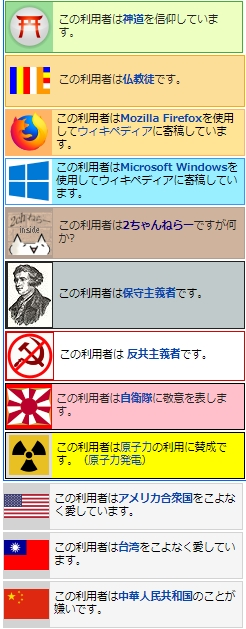
\includegraphics[width=\textwidth]{images/wiki/hashimoto.jpg}
  \caption{\textbf{User}: `S.S. Exp.Hashimoto' (Screenshot by author. Source: ja.wikipedia.org)}
  \label{fig:hashimoto}
 \end{subfigure}
  \begin{subfigure}[b]{0.3\textwidth}
  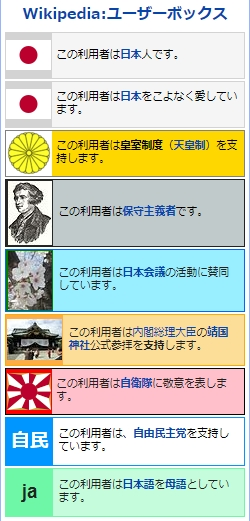
\includegraphics[width=\textwidth]{images/wiki/defense-corps.jpg}
  \caption{\textbf{User}: `護国防共団' (\textit{gokoku bōkyō-dan}) (Screenshot by author. Source: ja.wikipedia.org)}
  \label{fig:defense-corps}
 \end{subfigure}
 \begin{subfigure}[b]{0.3\textwidth}
  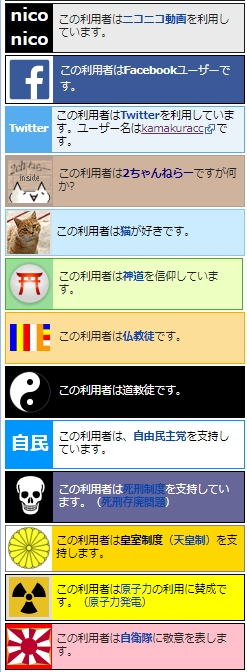
\includegraphics[width=\textwidth]{images/wiki/kamakura.jpg}
  \caption{\textbf{User}: `Kamakura' (Screenshot by author. Source: ja.wikipedia.org)}
  \label{fig:kamakura}
 \end{subfigure}
 \caption{Examples of Wikipedia Badges}\label{fig:badge-examples}
\end{figure}

The hyper-linked design of the MediaWiki software, reflecting on Azuma
(\protect\hyperlink{ref-azuma_otaku:_2001}{2001}) and Manovich
(\protect\hyperlink{ref-manovich_software_2013}{2013}), offers
previously unseen ways of global interconnection by linking articles
between the different language variants of Wikipedia. This has political
consequences as well. I have already shown the tendency of editing
articles on non-Japanese Wikipedia variants (primarily the English
variant) by several users depicting tropes common to the Netto-Uyoku.
Whereas the English article\footnote{The page was created on 2016-06-01
  with the most recent revision made on 2019-07-17.} portrays
Netto-Uyoku as ``Japanese neo-nationalists who interact almost entirely
within their own cyber community, shut off from the rest of Japanese
society'' and who ``first appeared on the Internet during the Lost
Decade, which was an economic crisis in Japan from the 1990s to 2010s''
(perpetuating the idea of Netto-Uyoku as a disenfranchised by-product of
the Lost Decade), on November 11, 2018 a user by the name of `Normal
Japanese' replaced the page contents with ``anti-Japanese left wings
will perish'' (which was reverted one minute afterwards). The normative
framing of oneself as ``normal Japanese,'' representing the general will
of the Japanese people, is a common red line throughout Netto-Uyoku
rhetoric, as is the usage of ``anti-Japanese left wings'' (a direct
translation of \emph{han'nichi sayoku}, 反日左翼) and `perish'
(\emph{shine}, 死ね) as aggressive verbal attack.\footnote{Adachi
  Yasushi (a House of Representatives member and Deputy Secretary
  General of Japan Innovation Party) for example, tweeted on 11 Nov 2017
  「朝日新聞、死ね。」 (\emph{asahi shimbun, shine}, lit. ``Asahi
  Shimbun, die.''), which has since gained traction on Twitter with the
  hashtag ``\#朝日新聞死ね'' (Adachi
  \protect\hyperlink{ref-adachi_eng._2017}{2017}).}

With heated tensions between Japanese and South Korean nationalists, it
is not unexpected to find traces of struggles online and on Wikipedia
either (as suggested by \textbf{figures \ref{fig:netto-altright}} and
\textbf{\ref{fig:netto-altright-kor}}). Although the page on Zaitokukai
has variants in different languages, the article on the umbrella term
for such organizations as the Action Conservative Movement is available
only on the Japanese and Korean Wikipedia. Another example of utilizing
interlinking articles for nationalist purposes: a large-scale DDoS
(cyber-)attack on 2channel's servers occurring on March 1, 2010 has an
article in Japanese (\emph{Kangokujin ni yoru 2-chan neru e no saibātero
jiken} `韓国人による2ちゃんねるへのサイバーテロ事件') and Korean
(\emph{2010nyeon han·il sam-iljeol saibeo gong-gyeog sageon}, `2010년
한·일 삼일절 사이버 공격 사건'). An English variant (`2010 Japan--South
Korea cyber-warfare') was created on December 24, 2014, 4 years after
the initial event, by a Korean-speaking user.\footnote{The English
  variant was created by user `Kanghuitari' (who has between April 29,
  2012 and July 11, 2019 contributed 27,984 edits on the English
  Wikipedia page and 28,411 edits on the Korean Wikipedia).} Translated
to English, the Japanese title of the page is more akin to ``the
cyber-terror incident on 2channel by South Koreans,'' explicitly using a
reference to terrorism as an ideologically motivated attack. The Korean
title then translates to ``The 2010 South Korea-Japan 3-1
cyber-attack,'' with 3-1 (\emph{sam-iljeol}, 삼일절) as an explicit
reference to the Korean March \nth{1} Movement in 1919.

Another common aspect of Wikipedia are lists or categories with
personally identified correlations. Take for example the categories
`Anti-Japanese sentiment in Korea' (containing 61 pages), its Japanese
equivalent \emph{Kankoku no han'nichi kanjō} 韓国の反日感情 (56
articles) and its Korean equivalent \emph{daehanmingug-ui ban-il
gamjeong} `대한민국의 반일 감정' (80 articles). The English page has an
additional ``See also: Category:Anti-Korean sentiment in Japan.'' tag
that is present neither on the Japanese nor Korean variants.\footnote{There
  are however equivalents for that category on both the Korean Wikipedia
  (\emph{ilbon-ui banhan gamjeong} 일본의 반한 감정, with 23 items) and
  the Japanese Wikipedia (\emph{hankan kanjō} 反韓感情, lit.
  \emph{`anti-Korean sentiment'} and \emph{hanchō kanjō} 反朝感情, lit
  \emph{`anti-South Korean sentiment'}, containing respectively 4 and 18
  items).} That latter category, Anti-Korean sentiment in Japan, then
contains 33 articles (including a link to 2channel), with edits made to
primarily by users who have expressed Korean identity or interest into
Korea in their user-pages (such as the user `Caspian blue'\footnote{This
  user appears to be Swedish but contributions are almost exclusively on
  Korean cultural or historical aspects.}). Between April and July
2019‎, an anonymous user made additions to several pages such as
Japanese idol Chiba Reiko\footnote{Since 2016 frequent Toranomon News
  guest Chiba Reiko did publish various works on the topic, such as the
  2016 ``\emph{Sayonara payoku ― chibarei ga mita sayoku no jittai}''
  『さよならパヨク---チバレイが見た左翼の実態---』 (lit. ``Farewell
  Payoku-The Actual Condition of the Left Wing As Seen by Chiba-Rei'')
  and the collaboration with Zaitokukai-founder Makoto Sakurai
  『くたばれパヨク』 (lit. ``Drop dead \emph{payoku}''), as well as the
  2017 ``\emph{mama ha aikoku}'' 『ママは愛国』 (lit. ``Mommy is a
  patriot'') with prolific right-wing author Kurayama Mitsuru and
  \emph{``kanashī sayoku ni goyōshin!''} 『悲しいサヨクにご用心!』 (lit.
  ``Beware of the sad left-wingers'') with Kurayama Mitsuru and LDP
  lawmaker Mio Sugita.} and film director and comedian Kitano Takeshi,
including the Wiki-formatted reference
`\texttt{[[Category:Anti-Korean sentiment in Japan]]}'. As of July 2019
Kitano Takeshi is still listed as belonging to this category, although
neither the English nor Japanese variant contain mentions of anti-Korean
sentiment either on the main document or in prior revisions).\footnote{Rumors
  of Takeshi Kitano having either anti-Korean sentiment or being
  ethnically Korean himself have been renewed in 2018, after a South
  Korean idol reportedly came under fire for posting on social media a
  gift he received from the film-maker. The Korea Times erroneously
  reported `anti-Korean Japanese filmmaker Kitano Takeshi' as having
  co-authored a book on the Senkaku Islands with Ishihara Shintaro in
  the early 2000s (Dong \protect\hyperlink{ref-dong_ikon_2018}{2018}).
  This was echoed by British outlet Metro (Hicap
  \protect\hyperlink{ref-hicap_ikons_2018}{2018}).}

The revision pages of those pages too confirm what I have thus far
demonstrated. Users are trying to influence public perception on
sensitive topics both regionally and internationally. Of note here is
the user \emph{`ao-oniyoshi'} (`青鬼よし'), with 7,662 edits on 2,192
articles between February 22, 2009 and July 9, 2019 and a top editor on
the Japanese article for `\emph{Hatoyama Yukio}' and `\emph{March
\nth{1} Movement}'. This user's edits include 577 edits on the English
Wikipedia, focusing primarily on the article for `Kofun period' (87),
`Japan--Korea disputes' (30) and `Korea under Japanese rule' (15) before
this account on the English Wikipedia was locked.\footnote{On the
  Japanese alternative MediaWiki website \emph{ja.yourpedia.org}, this
  is user is described in a dedicated page as \emph{neto-uyo-pedian}
  (「ネトウヨペディアン」).} Since then, a `Category:Suspected Wikipedia
sockpuppets of Azukimonaka' lists \emph{`ao-oniyoshi'} (`青鬼よし') as
one of 25 double accounts of one suspected user contributing edits to
controversial topics on Korean and Japanese history. Amongst the other
users in this list are the user `KoreanShoriSenyou' (which when written
in Japanese characters could refer to the account as intended
exclusively or possibly combatively for disposal or procession of
anything Korean-related, コリアン処理専用 or コリアン処理戦用) and
Azukimonaka (whose top edits include pages on `Eugenics in Japan',
`Foreign relations of South Korea', `Japanese expansionism' and `Manga',
as well as on the category of `Anti-Japanese sentiment in Korea').

\begin{figure}[!htb]
 \centering
 \begin{subfigure}[b]{1\textwidth}
 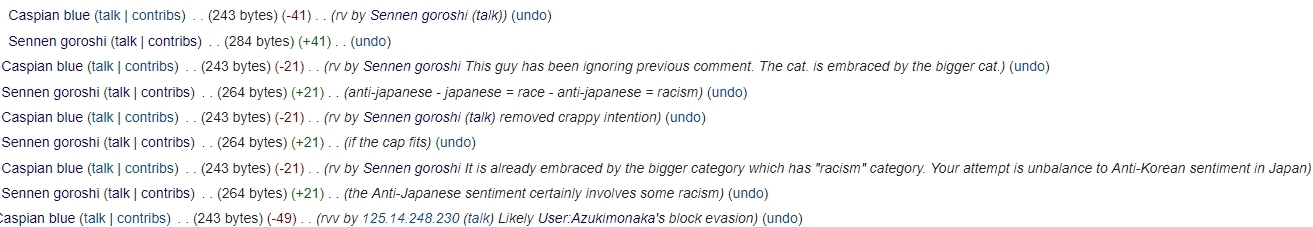
\includegraphics[width=0.95\textwidth,trim=4 4 4 4,clip]{images/wiki/sennen-caspian2.jpg}
  \caption*{(Screenshot by author. Source: ja.wikipedia.org)}
 \end{subfigure}
 \caption{\label{fig:caspian} Edit Skirmish on English Wikipedia Page 'Anti-Korean sentiment in Japan'.}
\end{figure}

Finally, another user, `Sennen goroshi' (which is when written in
Japanese, 千年殺し, a reference to a particular practical joke in the
animation Naruto) has made 4,837 edits on 1,588 English Wikipedia pages
between July 28, 2007 and June 16, 2019, dominantly on topics related to
Japanese and Korean nationalism. Yet this user does not appear to be
Japanese.\footnote{In order edits to the articles of `Comfort women',
  `Empress Myeongseong', `List of Nürburgring Nordschleife lap times'
  (the one exception in this list, a reference to a racking track in
  Germany), `Kimchi', `Korean cuisine', `Nanjing Massacre', `Kim Koo',
  `South Korea' and `Anti-Japanese sentiment in Korea'.} Nevertheless
does this user, on the English language Wikipedia page for `Anti-Korean
sentiment in Japan', engages in a brief edit-war with the aforementioned
user `Caspian blue', as seen on \textbf{figure \ref{fig:caspian}}.
Taking sides based arguably through the soft-power influence of both
South Korea and Japan,\footnote{This is of course not limited to
  controversial elements within Japan-Korea relations. On the English
  article for `Senkaku Islands', the American user `Washuotaku'
  (according to his Wikipedia profile a reference to the animation
  series `Tenchi Muyo!') has between September 2018 and January 2019
  regularly reverted edits in favor of Japan's asserted historical
  control.} two seemingly unrelated users thus attempt to tip the
balance in favor of a country they feel an imagined affiliation with.

\section{\texorpdfstring{Online Grassroots counter-Activism: `Ban
Matsuri'}{Online Grassroots counter-Activism: Ban Matsuri}}\label{online-grassroots-counter-activism-ban-matsuri}

As I have demonstrated in the first chapter, the world wide web and
social media platforms are increasingly relevant tools for shifting
public opinion. Moreover, this is done from the ideologically populist
stance that these media---\emph{bottom-up} media lacking so-called
gatekeepers---represent the people's will. In other words, a Habermasian
online public sphere on which counter-hegemonic ideologies have space to
develop and seep into civil society. In this chapter I demonstrated
several attempts to steer public opinion by those who reside in
2channel's most active echo-chambers. This was done on an active level
by using widespread tools as Wikipedia, but also passively through
reinforcement of what is framed as the people's voice on \emph{matome}
aggregation websites. Those aggregation websites should be noted for
being profit-driven and acting on a demand of (such-framed)
\emph{Japan-bashing}.

The consumption `anti-Japan' news serves discursive processes of
nationalist self-socialization through antagonistic Othering. In other
words, a construction of the self as being both morally superior to the
irrationality of the dehumanized Other, but also as the \emph{real}
victim of a greater anti-Japanese conspiracy driven by the leftist
elites, mainstream news and an imagined foreign enemy. This is further
framed in a cynicism adherent to these cyber-communities. Alongside the
blogs I have already mentioned, can the latter be deduced from the mere
names of certain aggregation blogs and channels: `Kimchi Newsflash'
(\emph{kimuchi sokuhō} 「キムチ速報」), `Traitor Newsflash'
(\emph{baikoku sokuhō}, 「売国速報(\^{}ω\^{})」), `Funny Anti-Japan
Channel' (\emph{omoshiro han'nichi chan'neru}
「おもしろ反日チャンネル」), `Zainichi Korean Crime Newsflash'
(\emph{zainichi hanzai sokuhō}, 「在日犯罪速報<丶`\(\forall\)´>」),
and `Mizuki's \emph{Girl Knowledge Korea Declaration}' (\emph{`Mizuki no
joshi chi Kan sengen'}, 「みずきの女子知韓宣言(´\(\forall\)`*)」). Of
note is the usage of \emph{emoji} signifiers in the latter three cases
here; another textual tool for making more accessible and appealing what
is in essence highly ideological rhetoric.\footnote{Blogger `Mizuki',
  who has over 221,000 followers on the aptly titled Twitter account
  @mizukikenkan (a transliteration of the Japanese \emph{kenkan} 嫌韓,
  `Hate Korea') holds a \emph{matome}-blog wherein she selectively
  translates Korean reactions to Naver news-articles. `Mizuki's twitter
  account states ``I love Japan. I hate anti-Japanese sentiment. I want
  to calmly keep an eye on the past and the future of this country while
  treating 'facts' as important.'' (\emph{Nihon ga daisukidesu.
  Han'nichi ga daikirai. 'Jijitsu' o daiji ni shite reisei ni kono kuni
  no kako to mirai o mitsumetai.},
  「日本が大好きです。反日が大嫌い。「事実」を大事にして冷静にこの国の過去と未来を見つめたい。」).
  The first article 'Mizuki' posted after an arson attack on an
  animation studio in Kyoto, Japan was on July 19, 2019 0:02 A.M.,
  titled ``{[}Korea's Reaction{]} `Die'. Splashed with gasoline\ldots{}
  The catastrophe of 33 deaths at Kyoto Animation Arson attack''
  (\emph{{[}Kankoku no han'nō{]} `shine' gasorin bukkake\ldots{} keiani
  hōka de 33-nin ga shibō no dai sanji'},
  「【韓国の反応】「死ね」ガソリンぶっかけ\ldots{}京アニ放火で33人が死亡の大惨事」)
  (Mizuki \protect\hyperlink{ref-mizuki_eng._2019}{2019}).}

Some of those media platforms have however reacted to those trends by
implemented specific terms of services that prohibit inciting violence
or hate. Users have the option to report content, and based on the
amount of reports will those platforms then automatically \emph{flag},
block or remove accounts and their associated content. The colloquial
`Netto-Uyoku ban' (ネトウヨBAN祭り \emph{neto-uyo ban matsuri}, lit.
`Netto-Uyoku Ban Festival') is one such instance of grassroots activism
based around those methods (In the context of \emph{2channel},
\emph{matsuri} 祭り refers to a large-scale online meeting with a
particular ideological purpose, such as `attacking' a self-perceived
other). The \emph{Asahi Shimbun} reported in 2018 a large scale deletion
of YouTube channels, including that of Toranomon News regular Takeda
Tsuneyasu (Shino \protect\hyperlink{ref-shino_eng:_2018}{2018}). A trend
amongst deleted videos was the usage of automated voices and text
scrolling over a black background or several images. Furthermore, a look
at the list of removed accounts reveals a slight majority of accounts
with unrelated Western usernames (such as the most recent deleted
accounts `Sandy Kerrigan', `Beauty Eansworth', `Erica Bray' and `Vickie
Cooper'), with a high ratio of uploaded videos in comparison to the
amount of subscribers (ハンJ Wiki
\protect\hyperlink{ref-j_wiki_completed_2019}{2019}), which strongly
suggests the usage of double accounts (\emph{sockpuppets}) and bots, as
referred to in chapter two by Schäfer, Evert, and Heinrich
(\protect\hyperlink{ref-schafer_japans_2017}{2017}).

This was followed by a \emph{Sankei Shimbun} tabloid reporting over 2000
YouTube channels and 2000 Twitter accounts suspended (including that of
Zaitokukai's Sakurai Makoto), with over 50 million tweets deleted and
cited damage to channels such as \emph{Bōkoku no ījisu}
(「某国のイージス」, lit. `A Certain Country's Isis'),\footnote{This
  user runs a Twitter-account @defendjapan and is the owner of the above
  mentioned YouTube accounts `Funny Anti-Japan Channel' (\emph{omoshiro
  han'nichi chan'neru} 「おもしろ反日チャンネル」) and the English
  「Good morning Korea channel」. Both channels remain as of 16-07-2019
  unaccessible. Moreover, this user has contributed writings to at least
  16 different volumes of Japanism.} that of Kazuya and Toranomon News
(Ogawa \protect\hyperlink{ref-ogawa_eng._2019}{2019}) and Tony Marano
(known as \emph{tekisasu oyaji} テキサス親父 or `Texas
Daddy').\footnote{As the content is not explicitly, verbally
  classifiable as inciting hate or violence, the accounts of Takeda
  Tsuneyasu, Kazuya and Toranomon News have since been restored.} In a
final diversion, the latter is worth expanding upon as another source of
`foreign' reconfirmation. Various publications have been accredited to
Tony Marano, including several columns in Japanism, a book co-authored
by Toranomon News associate Kent Gilbert (『素晴らしい国・日本に告ぐ!』
\emph{Subarashī kuni ・ Nihon ni tsugu!}, lit. ``Wonderful Country, I'll
Inform japan!'') and an article co-authored by Hyakuta Naoki
(「朝日の慰安婦報道を断罪する!」 \emph{Asahi no ianfu hōdō o danzai
suru!}, lit. ``We condemn the Asahi Comfort Women Report!'').\footnote{The
  latter was published by the monthly magazine \emph{WiLL}, whose
  regular contributors include Toranomon News hosts and regular guests
  Fujii Genki, Kent Gilbert, Seki Hei, Jōnen Tsukasa and Sakurai
  Yoshiko. It wouldn't be far-fetched to claim a pattern here.} On his
main English account `PropagandaBuster' Tony Marano writes ``In an
attempt to counter political correctness from the news media, I will
examine propaganda masquerading as truth in the America news media. Also
explore and expose the mental disorder of liberalism and political
correctness infecting Hollywood, academia, and the re-education camps
(public schools). Unchecked far left liberals in the United States are
the single cause for the rapid decline of this nation, we must counter
their leftist, anti-American ideology on every level.'' A textbook
example of neo-nationalism on the Internet, and if translated in a
Japanese context, a textbook example of Netto-Uyoku.\footnote{On
  2019-07-16, a YouTube Japan search (on an unrelated IP address and
  device, not logged in YouTube, to ensure my results were unaffected by
  my personal Google search queries.) for 「韓国」 (South Korea) and
  「日本」 (Japan) did respectively return his latest video
  「字幕【テキサス親父】 韓国に「恩を仇で返される」日本」 (\emph{jimaku
  {[}Tekisasu oyaji{]} Kankoku ni `on o kyū de kaesa reru' Nihon}, lit.
  ``Subtitled 【Texas daddy】 This is how South Korea repays Japan?'')
  as the \nth{3} and \nth{4} result.}

The users behind the `Netto-Uyoku ban' are users that identify
themselves with particular subcategories of \emph{2channel}, including
the aforementioned \emph{kenmō} board (「嫌儲」), the Korean-centered
board \emph{hanguru} (「ハングル」) and a board designed for the
discussion of baseball \emph{Nandemo jikkyō (jupitā)} 「なんでも実況
(ジュピター)」. Moreover, while discussion on their activities happens
on 2channel, they are they using MediaWiki software to organize
themselves and inform on grassroots-level methods to counter what they
deem to be Netto-Uyoku carriers of hate-speech. Those users have not
just reported and documented YouTube and Twitter accounts they deemed
belonging to Netto-Uyoku users, but by reporting blogs and other
websites using means like Google's Adsense, they effectively block the
income of such accounts. Furthermore, on their Wiki-homepage they have
explicitly called out for the revision of Netto-Uyoku leaning Wikipedia
articles (「ネトウヨのウィキペディアの偏向記事を改善するんだ」
``\emph{neto-uyo no wikipedia no henkō kiji o kaizen surunda}'', lit.
``We're improving the Wikipedia articles with Netto-Uyoku
inclinations'') (hangul.shoutwiki.com
\protect\hyperlink{ref-hangul.shoutwiki.com_wikipedia_2019}{2019}).

\section{Conclusion}\label{conclusion-2}

Like elsewhere in the world, Wikipedia as a platform and the software
structure behind it are increasingly relevant to Japanese Internet
users' methods for informing oneself. Nevertheless, as demonstrated on
the previous pages political topics are dominantly revised by a small
group of Wikipedia users in order to express political ideology and
influence the public opinion. I have further shown ties between editors
on the Japanese Wikipedia and 2channel, both in methods of organization
(high tendencies for editing anonymously as well as using MediaWiki
platforms for meta-discussions on Wikipedia) and in taking one's usage
of \emph{2channel} as a source of pride and identity. Neither are these
users expressing their interests on Wikipedia exclusively around
political topics either, with either having a history of editing topics
on popular culture, or explicitly referencing those topics on their
profile. The dominance of Japanese popular culture and the soft-power
strategy of Cool Japan is further proven by the high percentage of
articles\footnote{In a \emph{New York Times} interview, Wikipedia
  co-founder Jimmy Wales claimed that 80 percent of Japanese Wikipedia
  articles were devoted to pop culture (Cohen
  \protect\hyperlink{ref-cohen_wikipedia_2009}{2009}).} and edits
devoted to popular culture topics like Japanese animation and idol
formations. The time-line of increase in edits on contentious topics
then too generally falls in line with my hypothesis of populist
neo-nationalism becoming the hegemonic ideology during the crucial years
of 2009 - 2011. Moreover, due to the ease of intersection with other
language versions of Wikipedia, the most dedicated among those editors
attempt the same thing on a global scale. Something that is not done
solely as an expression of (Japanese) nationalism, either. The
international reach of soft-power strategies for disseminating the
hegemonic ideology lead to such phenomena of neither ethnically Korean
or Japanese citizens trying to tip the balance of information-making in
favor of either nation.

Channeling McLuhan, Azuma
(\protect\hyperlink{ref-azuma_otaku:_2001}{2001}) and Manovich
(\protect\hyperlink{ref-manovich_software_2013}{2013}) I've further
drawn attention to the technical structure of the software behind some
of these cyber-communities in which self-socialization and dispersion of
ideology occurs. That is to say, imagined cyber-communities build around
shared ideological values and utilizing normative rhetorical devices for
influencing public opinion on the Internet as a public sphere.
Capitalizing on the early growth of cyber-nationalism on the most active
of 2channel's boards, so called curated \emph{matome} blogs started
aggregating content as being representative of the online voice, adding
attractive titles to draw in clicks and increase profit through online
advertisements. In protest, parts of those sub-communities relocated and
started viewing the previous board as their imagined Other, resulting in
a polarizing effect amongst its users and enhancing the echo-chamber
effect of the communities \emph{matome} blogs aggregate. As illustrated,
this has the potential to spread like wildfire, enforcing political
biases on a global scale.

As cyber-nationalists normalized their ideology spread throughout civil
society, backed by politicians and capitalized on by populist right-wing
influencers such as those of Toranomon News, so too then did a
counter-ideological grassroots movement attempt to disrupt these trends.
One such expression, the `Ban Matsuri', while still rooted in the
contrarian `new frontier' ideology of the World Wide Web, was formed by
users of the same 2channel community, including those that were deterred
from being aggregated profit-seeking \emph{matome} blogs. Using
MediaWiki for the organization and administration of their
counter-activism, their actions have led to the removal of income for
influential news-aggregation websites and the deletion of thousands of
public YouTube and Twitter accounts, affecting Toranomon News affiliates
as well.

\newpage

\chapter*{Conclusion}\addcontentsline{toc}{chapter}{Conclusion}

In my introductory first chapter, I bring the phenomenon of the
Netto-Uyoku to a global level as a localized expression of what I call
cyber-nationalists, and draw parallels with other such online instances
in the United States and Belgium. I further made the argument that the
Internet has seen increasing politicization; ranging from populist usage
of big-data and paid propaganda campaigns operating as \emph{faux}
grassroots activism, to microcosmic counter-culture subcultures;
primarily built (under the influence of Japan's soft power) around the
discussion of Japanese pop-culture and disrupting the public discourse
on political issues. In that chapter I next listed several questions I
intended to answer during this paper:

\begin{itemize}
\tightlist
\item
  What is the \emph{modus operandi} of the Netto-Uyoku to disseminate
  ideology?
\item
  What are the structural processes of the media platforms that the
  Netto-Uyoku utilize?
\item
  How do the Netto-uyoku compare to other online-based neo-nationalist
  movements? Can we speak of a distinct Japanese character compared to
  contemporary movements, or should we view the Netto-Uyoku primarily as
  part of a greater trend of Internet-fueled populist neo-nationalism?
  Secondly, is there a common reaction to, for example, the Alt-Right
  and Trump-era politics?
\item
  How does the movement organize and mobilize, both online and in real
  life?
\item
  Is there possible space for furthering a Netto-Uyoku political
  ``agenda'' through influencing its international counterparts?
\end{itemize}

The term Netto-Uyoku was coined fifteen years ago. In my second chapter
I have reviewed a select amount of literature both from the early period
covering the Netto-Uyoku as a fringe element of greater topics, to more
recent literature covering the Netto-Uyoku and the Internet.

In the third chapter, I attempted to map the ideology behind the
right-wing reactionary voices utilizing the Internet, drawing on
Frankfurt School scholars' theorization of ideology and media. It is a
pitfall to apply theory rooted in western cultural traditions without
balancing the different socio-cultural contexts of the subject, and
arguments could be made against the continuous western hegemony of
academia. Yet, when we follow Anderson's and McLuhan's logic on media
and literacy as crucial to nationalism, and see the world as a `global
village' connected by the digital, it wouldn't be a far stretch to
consider the universal nature of the concepts presented in this chapter.

While I could never claim information warfare, populist demagoguery or
nationalism to be new tactics in politics, this is now done to great
success on the Internet; fueled by both the technological peculiarities
of the Internet itself and the rhetoric formed on Internet subcultures.
In the fourth chapter I covered the development of Japanese Internet
subcultures and the close ties of Otaku culture with the adaption of the
Internet.

https://www.buzzfeednews.com/article/ryanhatesthis/brazil-jair-bolsonaro-facebook-elections

In the third chapter, I found many of the ideological goals of the
Netto-Uyoku to fall in line with that of the current administration, who
have in turn done well in dog-whistling to the Netto-Uyoku. This could
be interpreted as one reason for a lack of political success for the
Netto-Uyoku-associated Makoto Sakurai and his Japan First Party.

I conclude that the Netto-Uyoku, like its counterparts across the world,
is on one hand a continuation of an ideological war

Whereas the rise in global right-wing populism shook the world in 2016,
which falls in line with the wide-spread counter-hegemonic narrative
disseminated in part by cyber-nationalists, I argued that this has
appeared much earlier in Japan. More specifically in an outburst of
public outrage after events occurring around 2011: scandals in politics,
public media and the 2011 Fukushima Nuclear Disaster (as suggested on
page \pageref{populism-gt} by \textbf{Figure \ref{fig:politictrends}}).
\emph{Interest}\footnote{Another interesting expression considering this
  very word is rooted in capitalist commodity fetishism.} in politics
has taken an increasingly large relative share of Google searches across
the world. In Japan, interest has remained relatively stable with the
exception of a massive peak in 2011; A massive peak noted by the way on
\textbf{Figure \ref{fig:nettouyoku}} (page \pageref{nettouyoku-gt}).

Following various contradictions in post-war Japan's society, The New
Left and student protests influenced by Marxist scholars shook civil
society. Now, anti-intellectual right-wing populists are
(sub-)consciously applying the same Marxist school of thought.
Contradictions in society, most notably the effects of alienation in the
wake of the Lost Decades, have renewed public distrust. Within this
sphere of alienation and crises of identity, digital natives built
intrinsic cyber-communities with a distinct anti-establishment
discourse---a cyber-discourse with vast ties to the libertarian mindset
that shaped the ideology behind the Internet in the first place.

As we see happening across the world, I argued these communities to be
ripe for political exploitation (in the form of a potential political
electorate) by those same right-wing populists. Whether its Donald
Trump's presidential campaigns, Duterte in the Philippines or the
Flemish right-wing populist Vlaams Belang in 2019, right-wing populists
have since the second half of the 2010 gained considerable support
throughout the world by including digital natives in their campaign
strategies. Distinct from national-scale politics in the United States
however, I conclude that in Japan the current iteration of the LDP
administration has successfully capitalized on this public distress.
Although perceived societal contradictions up to the `90s shook the core
of the LDP strong enough to bring about a massive reform of the voting
system, I next argued that from the '90s onwards societal contradictions
between the 'hegemonic ideology' and the perceived reality (seen to its
inevitable conclusion following the 2011 Fukushima Nuclear Disaster and
the reveal of the North Korean kidnappings) brought about a new
iteration of the LDP, or rather one that answered to the
counter-hegemonic narrative of the Japanese cyber-nationalists. The
actions of the Netto-Uyoku and the Zaitokukai have let to \emph{public}
disavowal by Abe Shinzo, yet on social media the prime minister uses
\emph{dog-whistling} methods to appeal to those groups by expanding
(\textbf{op inspelen}) upon those groups' rising concerns and
antagonizing enemies on common ground: established forms of media,
conservation of the ethnic-Japanese identity, and hostile positions
towards both the Korean peninsula and China. Perhaps in this sense Steve
Bannon had a point after all?

Finally I have demonstrated a higher awareness of group identity amongst
those who reject the Netto-Uyoku. If the Netto-Uyoku exist and are to be
named, then those who have become aware of this phenomenon and feel
rejection form a group identity too, both in the off-line public sphere
as on the Internet. Offline we have of course various counter protests
such as SealDs, C.R.A.C. and influenced by its Western counterparts, the
Antifa. Online we have seen communities form around exposing and
removing Netto-Uyoku means of radicalization (I refer in particular to
the 2018 - 2019 neto-uyo Ban Festival). It is premature to claim, but
perhaps this too can be seen as a trend of greater political shifts?

As hinted at throughout this paper, Netto-Uyoku are constantly fueled by
a source of perceived anti-Japanese sentiment coming from in particular
South-Korea and China; nations that are plagued by their own localized
expressions of cyber-nationalism and `troll-armies'. For future
research, this paper suggests a comparative analysis between those,
their \emph{modus operandi} and their interaction.

\newpage

\begingroup
\chapterstyle{thatcher}

\chapter*{References}\addcontentsline{toc}{chapter}{References}

\setlength{\parindent}{-0.2in} \setlength{\leftskip}{0.2in}
\setlength{\parskip}{0em} \noindent

This document utilizes the author-date citation system of The Chicago
Manual of Style 16th Edition (commonly referred to as \textbf{Chicago
B}).

\vspace{4mm} \setlength{\parskip}{0em} \footnotesize

\hypertarget{refs}{}
\hypertarget{ref-2021_summer_vs_2014}{}
2021 summer. 2014. 橋下徹vs在特会・桜井誠 【全】10/20.
\url{https://www.youtube.com/watch?v=ACRxHAC-tyg\&feature=youtu.be}.

\hypertarget{ref-5ch.net_eng._2016}{}
5ch.net. 2016. Eng. I'm Thinking About Bringing About a Labor Revolution
in This Rotten Country Japan. Violence Is Out of the Question. What Can
We Do?". \emph{Fox.5ch.net/Poverty/}.
\url{https://fox.5ch.net/test/read.cgi/poverty/1456058853/}.

\hypertarget{ref-5ch.net_eng._2019}{}
---------. 2019. Eng. Why Didn't the Hate Profit Board Didn't
Consistently Become Netto-Uyoku? I Think There Lies a Secret for Not
Become Netto-Uyoku. \emph{Leia.5ch.net/Poverty/}.
\url{http://2ch-ranking.net/cache.php?thread=leia.5ch.net/poverty/1563124016/\&res=100}.

\hypertarget{ref-abe_1_2012}{}
Abe, Shinzō. 2012. (1) Shinzo Abe-the Election to Decide the Future of
Japan Will Start Tomorrow. Rising China Will Not Hide from Japan Its
Territorial Ambitions ...
\url{https://www.facebook.com/photo.php?fbid=272889402834510\&set=a.131635893626529\&type=1\&theater}.

\hypertarget{ref-adachi_eng._2017}{}
Adachi, Yasushi. 2017. Eng. `Asahi Shimbun, Die.' (Editorial) Towards
the Educational Opening of 'Kake', It Is Not Settled with This. Tweet.
\emph{@Adachiyasushi}.
\url{https://twitter.com/adachiyasushi/status/929462477770723328?ref_src=twsrc\%5Etfw}.

\hypertarget{ref-noauthor_advertise_nodate}{}
Advertise - 4chan. 2019. Accessed June 13.
\url{https://www.4chan.org/advertise}.

\hypertarget{ref-alexa_alexa_2019}{}
Alexa. 2019. Alexa - Nicovideo Competitive Analysis, Marketing Mix and
Traffic. \emph{Alexa}.
\url{https://www.alexa.com/siteinfo/nicovideo.jp}.

\hypertarget{ref-noauthor_alexa_2019}{}
Alexa - Top Sites in Japan - Alexa. 2019. \emph{Alexa}.
\url{https://www.alexa.com/topsites/countries/JP}.

\hypertarget{ref-anderson_imagined_2006}{}
Anderson, Benedict R. O'G. 2006. \emph{Imagined Communities: Reflections
on the Origin and Spread of Nationalism}. Rev. ed. London ; New York:
Verso.

\hypertarget{ref-anonymous_post_eng._2019}{}
Anonymous Post. 2019. Eng. 【Korean Youtuber】 Destroying a Ticket for
Japan at the Airport `This Is What a Real Boycot Is Like', Ticket or
Hotel Can Not Be Canceled Either {[}7/11{]}~The Internet Reacts 'Nah,
If You've Paid the Purchase Is Already Settled, Right?w' 'Paying and Not
Coming... You're the Best'. \emph{アノニマスポスト}.
\url{https://anonymous-post.mobi/archives/10853}.

\hypertarget{ref-aoki_virtual_1994}{}
Aoki, Kumiko. 1994. VIRTUAL COMMUNITIES IN JAPAN. In.
\url{https://www.ibiblio.org/pub/academic/communications/papers/Virtual-Communities-in-Japan}.

\hypertarget{ref-arimoto_eng._2019}{}
Arimoto, Kaori. 2019. Eng. {[}Arimoto Kaori's Fighting Poison with
Poison{]} "the Cherry Blossom Viewing Party'' an Amazing Assertion by
Tokyo Shimbun! Right, Left, Netto-Uyoku ... This Scary Writing,
Somewhere...? Article.society.domestic. \emph{Zakzak}.
\url{https://www.zakzak.co.jp/soc/news/190419/soc1904190003-n1.html}.

\hypertarget{ref-audureau_les_2017}{}
Audureau, William. 2017. Les Trolls Sur Internet, Nouveaux « Colleurs
d'affiches » Du Front National, March.
\url{https://www.lemonde.fr/pixels/article/2017/03/31/les-trolls-sur-internet-nouveaux-colleurs-d-affiches-du-front-national_5103959_4408996.html}.

\hypertarget{ref-azuma_otaku:_2001}{}
Azuma, Hiroki. 2001. \emph{Otaku: Japan's Database Animals}. 講談社.

\hypertarget{ref-azuma__2007}{}
---------. 2007. \emph{ゲーム的リアリズムの誕生}. 東京: 講談社.

\hypertarget{ref-azuma_ippan_2011}{}
---------. 2011. \emph{Ippan Ishi 2.0: Rusō, Furoito, Gūguru}. Tōkyō:
Kōdansha.

\hypertarget{ref-barubora_eng:_2017}{}
Barubora, and Sayawaka. 2017. \emph{Eng: Our History of Internet}.
亜紀書房.

\hypertarget{ref-baudrillard_simulacra_1994}{}
Baudrillard, Jean. 1994. \emph{Simulacra and Simulation}. The Body, in
Theory. Ann Arbor: University of Michigan Press.

\hypertarget{ref-benedictus_invasion_2016}{}
Benedictus, Leo. 2016. Invasion of the Troll Armies: `Social Media Where
the War Goes on'. \emph{The Guardian}, November.
\url{https://www.theguardian.com/media/2016/nov/06/troll-armies-social-media-trump-russian}.

\hypertarget{ref-bo-gyung_youtube_2019}{}
Bo-gyung, Kim. 2019. YouTube, a New Conservative-Liberal Battle Ground.
\emph{The Korea Herald}.
\url{http://www.koreaherald.com/view.php?ud=20190106000203}.

\hypertarget{ref-brewster_after_2019}{}
Brewster, Thomas. 2019. After the New Zealand Terror Attack, Here's Why
8chan Won't Be Wiped from the Web. \emph{Forbes}.
\url{https://www.forbes.com/sites/thomasbrewster/2019/03/15/after-the-new-zealand-terror-attack-should-8chan-be-wiped-from-the-web/}.

\hypertarget{ref-bungeishunju_editorial_department_eng._2019}{}
Bungeishunjū editorial department. 2019. Eng. Shibata Shigeru Rages, LDP
Headquarters Distributes `Neto-Uyo Book' to All Members.
\emph{文春オンライン}. \url{https://bunshun.jp/articles/-/12725}.

\hypertarget{ref-buttigieg_gramsci_1995}{}
Buttigieg, Joseph A. 1995. Gramsci on Civil Society. \emph{Boundary 2}
22 (3): 1. doi:\href{https://doi.org/10.2307/303721}{10.2307/303721}.

\hypertarget{ref-cerulus_inside_2019}{}
Cerulus, Laurens. 2019. Inside the Far Right's Flemish Victory.
\emph{POLITICO}.
\url{https://www.politico.eu/article/inside-the-far-rights-flemish-victory/}.

\hypertarget{ref-ceulaer_6_2016}{}
Ceulaer, Joël De. 2016. 6 Ongemakkelijke Waarheden over Vlaams Belang.
\emph{De Morgen}. \url{https://www.demorgen.be/gs-b100aaff}.

\hypertarget{ref-chandler_act_1995}{}
Chandler, Daniel. 1995. \emph{The Act of Writing: A Media Theory
Approach}. Aberystwyth: University of Wales.

\hypertarget{ref-charity_why_2016}{}
Charity, Justin. 2016. Why Do Anonymous Twitter Trolls Use Anime
Avatars? \emph{The Ringer}.
\url{https://www.theringer.com/2016/8/9/16046698/anonymous-twitter-trolls-anime-avatars-harassment-4chan-8578d36b2920-8578d36b2920}.

\hypertarget{ref-chokshi_reddit_2019}{}
Chokshi, Niraj, and Neil Vigdor. 2019. Reddit Restricts Pro-Trump Forum
Because of Threats. \emph{The New York Times}, June.
\url{https://www.nytimes.com/2019/06/26/us/politics/reddit-donald-trump-quarantined.html}.

\hypertarget{ref-chosun.com_japanese_2011}{}
Chosun.com. 2011. Japanese March Against Korean Soap Operas, August.
\url{http://english.chosun.com/site/data/html_dir/2011/08/22/2011082200679.html}.

\hypertarget{ref-cnn_korean_2010}{}
CNN. 2010. Korean Cyber Attack on 2ch CNN Travel.
\emph{CNN}.\href{./}{/}.

\hypertarget{ref-cohen_wikipedia_2009}{}
Cohen, Noam. 2009. Wikipedia Looks Hard at Its Culture. \emph{The New
York Times}, August.
\url{https://www.nytimes.com/2009/08/31/business/media/31link.html}.

\hypertarget{ref-collins_anti-semitic_2019}{}
Collins, Ben, and Andrew Blankstein. 2019. Anti-Semitic Open Letter
Posted Under Name of Synagogue Shooting Suspect. \emph{NBC News}.
\url{https://www.nbcnews.com/news/us-news/anti-semitic-open-letter-posted-online-under-name-chabad-synagogue-n999211}.

\hypertarget{ref-daelyugnamtv_eng._2019}{}
daelyugnamTV. 2019. Eng. `I Tore a Ticket of 1.35 Million Won.'
\url{https://www.youtube.com/watch?v=sO7B6V0ho6M\&feature=youtu.be}.

\hypertarget{ref-darcy_obama_2016}{}
Darcy, Oliver. 2016. Obama on Trump: 'I Don't Think He's Ideological'.
\emph{Business Insider}.
\url{https://www.businessinsider.com/obama-trump-ideological-pragmatic-2016-11}.

\hypertarget{ref-davison_language_2012}{}
Davison, Patrick. 2012. The Language of Internet Memes. In, 120--34.

\hypertarget{ref-van_dijk_politics_2006}{}
Dijk, T A van, and Universitat Pompeu Fabra. 2006. Politics, Ideology,
and Discourse. \emph{The Encyclopedia of Language and Linguistics.}, no.
9: 13.

\hypertarget{ref-dong_ikon_2018}{}
Dong, Dong. 2018. iKON Member Under Fire for Backing Kitano Takeshi.
\url{https://m.koreatimes.co.kr/pages/article.asp?newsIdx=256071}.

\hypertarget{ref-dougherty_new_2016}{}
Dougherty, Michael Brendan. 2016. A New Nationalism Is Rising. Don't Let
Donald Trump Destroy It.
\url{https://theweek.com/articles/638440/new-nationalism-rising-dont-let-donald-trump-destroy}.

\hypertarget{ref-dower_peace_1993}{}
Dower, John W., GARY D. ALLINSON, SANDRA BUCKLEY, BRUCE CUHINGS, JOHN W.
DOWER, SHELDON GARDON, CAROL GLUCK, et al. 1993. Peace and Democracy in
Two Systems: External Policy and Internal Conflict. In \emph{Postwar
Japan as History}, 3--33. University of California Press.
\url{http://www.jstor.org/stable/10.1525/j.ctt1pp638.5}.

\hypertarget{ref-eagleton_ideology:_1991}{}
Eagleton, Terry. 1991. \emph{Ideology: An Introduction}. London ; New
York: Verso.

\hypertarget{ref-ellis_4chan_2018}{}
Ellis, Emma Grey. 2018. 4Chan Is Turning 15---And Remains the Internet's
Teenager. \emph{Wired}, June.
\url{https://www.wired.com/story/4chan-soul-of-the-internet/}.

\hypertarget{ref-fackler_new_2010-1}{}
Fackler, Martin. 2010. A New Wave of Dissent in Japan Is Openly and
Loudly Anti-Foreign. \emph{The New York Times}, August, Page A6.

\hypertarget{ref-fackler_japanese_2013}{}
---------. 2013. Japanese Court Fines Rightist Group over Protests at a
School in Kyoto:~{[}Foreign Desk{]}. \emph{New York Times,~Late Edition
(East Coast)}, October. New York, N.Y., United States, A.10.
\url{http://www.nytimes.com/2013/10/08/world/asia/japanese-court-fines-rightist-group-in-elementary-school-protest.html}.

\hypertarget{ref-fairclough_media_2010}{}
Fairclough, Norman. 2010. \emph{Media Discourse}. Repr. London:
Bloomsbury Academic.

\hypertarget{ref-feuer_founder_2018}{}
Feuer, Alan, and Ali Winston. 2018. Founder of Proud Boys Says He's
Arranging Surrender of Men in Brawl. \emph{The New York Times}, October.
\url{https://www.nytimes.com/2018/10/19/nyregion/the-proud-boys-gavin-mcinnes-arrested.html}.

\hypertarget{ref-flath_japanese_2005}{}
Flath, David. 2005. \emph{The Japanese Economy}. 2nd ed. Oxford,
England; New York: Oxford University Press.

\hypertarget{ref-freeman_meet_2016}{}
Freeman, Philip, ContributorClassics professor, and author. 2016. Meet
the Trump of Ancient Rome, a Populist Demagogue Who Helped Bring down
the Republic. \emph{HuffPost}.
\url{https://www.huffpost.com/entry/trump-rome-populist_b_9659660}.

\hypertarget{ref-fuchs_racism_2018}{}
Fuchs, Christian. 2018. Racism, Nationalism and Right-Wing Extremism
Online: The Austrian Presidential Election 2016 on Facebook. In,
157--206. University of Westminster Press.
doi:\href{https://doi.org/10.16997/book30.i}{10.16997/book30.i}.

\hypertarget{ref-furuta_eng:_2018}{}
Furuta, Daisuke, and Takumi Harimaya. 2018. Eng: The Reason Why I
Support `Hoshu Sokuho', We Lsten to the Assertion of a Blogging
Councilor. \emph{BuzzFeed}.
\url{https://www.buzzfeed.com/jp/takumiharimaya/hosyusokuhou-shinya-kotsubo}.

\hypertarget{ref-furuya_roots_2016}{}
Furuya, Tsunehira. 2016a. The Roots and Realities of Japan's
Cyber-Nationalism. \emph{Sasakawa USA}.
\url{https://spfusa.org/nippon-com/the-roots-and-realities-of-japans-cyber-nationalism/}.

\hypertarget{ref-furuya_can_2016}{}
---------. 2016b. Can Laws Control Japan's Hate Epidemic?
\emph{Nippon.com}. \url{http://www.nippon.com/en/currents/d00224/}.

\hypertarget{ref-gill_nativist_2018}{}
Gill, Tom. 2018. The Nativist Backlash: Exploring the Roots of the
Action Conservative Movement. \emph{Social Science Japan Journal} 21
(2): 175--92.
doi:\href{https://doi.org/10.1093/ssjj/jyy023}{10.1093/ssjj/jyy023}.

\hypertarget{ref-gotev_vlaams_2018}{}
Gotev, Georgi. 2018. Vlaams Belang Hosts Steve Bannon, Marine Le Pen in
Flemish Parliament. \emph{Euractiv.com}.
\url{https://www.euractiv.com/section/eu-elections-2019/news/vlaams-belang-hosts-steve-bannon-marine-le-pen-in-flemish-parliament/}.

\hypertarget{ref-gramsci_selections_1985}{}
Gramsci, Antonio, and Quintin Hoare. 1985. \emph{Selections from the
Prison Notebooks of Antonio Gramsci}. 8. pr. New York: International
Publ.

\hypertarget{ref-hachima_kiko_eng:_2019}{}
Hachima Kiko. 2019. Eng: `This Is What a Real Boycot Is Like!' Korean
Youtuber Takes the Effort to Destroy Plane-Ticket to Japan at the
Airport. \url{http://blog.esuteru.com/archives/9345531.html}.

\hypertarget{ref-hack_subculture_2016}{}
Hack, Brett. 2016. Subculture as Social Knowledge: A Hopeful Reading of
Otaku Culture. \emph{Contemporary Japan} 28 (March).
doi:\href{https://doi.org/10.1515/cj-2016-0003}{10.1515/cj-2016-0003}.

\hypertarget{ref-hangul.shoutwiki.com_wikipedia_2019}{}
hangul.shoutwiki.com. 2019. 【Wikipedia】改善対象記事 - ハンJ Wiki.
\url{http://hangul.shoutwiki.com/wiki/\%E3\%80\%90Wikipedia\%E3\%80\%91\%E6\%94\%B9\%E5\%96\%84\%E5\%AF\%BE\%E8\%B1\%A1\%E8\%A8\%98\%E4\%BA\%8B}.

\hypertarget{ref-harding_japan_2017}{}
Harding, Robin. 2017. Japan Passes Pre-Emptive Anti-Terrorism Law.
\emph{Financial Times}.
\url{https://www.ft.com/content/75130598-5181-11e7-bfb8-997009366969}.

\hypertarget{ref-hatachi__2018}{}
Hatachi, Kota. 2018. エプソンが保守速報への広告掲載をやめた
「嫌韓、嫌中の温床」との通報がきっかけに. \emph{BuzzFeed}.
\url{https://www.buzzfeed.com/jp/kotahatachi/hoshusokuho}.

\hypertarget{ref-he-rim_firebrand_2018}{}
He-rim, Jo. 2018. Firebrand Politician Hong Joon-Pyo Returns as
YouTuber. \url{http://www.koreaherald.com/view.php?ud=20181224000587}.

\hypertarget{ref-hess_how_2017}{}
Hess, Amanda. 2017. How the Trolls Stole Washington. \emph{The New York
Times}, February.
\url{https://www.nytimes.com/2017/02/28/magazine/how-the-trolls-stole-washington.html}.

\hypertarget{ref-hicap_ikons_2018}{}
Hicap, Jonah. 2018. iKON's Junhoe Apologises After Being Called Out by
Fan over Japanese Comedian. \emph{Metro}.
\url{https://metro.co.uk/2018/09/26/ikons-junhoe-apologises-after-being-called-out-by-fan-over-japanese-comedian-ahead-of-groups-comeback-7980418/}.

\hypertarget{ref-higuchi_japans_2014}{}
Higuchi, Naoto. 2014. Japan's Far Right in East Asian Geopolitics: The
Anatomy of New Xenophobic Movements. \emph{Social Science Research,
University of Tokushima} 28: 163--83.
\url{https://www.researchgate.net/profile/Naoto_Higuchi/publication/280727862_Japan's_Far_Right_in_East_Asian_Geopolitics_The_Anatomy_of_New_Xenophobic_Movements/links/55c337df08aeb975673e5d31.pdf}.

\hypertarget{ref-higuchi_japans_2016}{}
Higuchi, Naoto, and Teresa Castelvetere. 2016. \emph{Japan's
Ultra-Right}. Japanese Society Series. Melbourne: Trans Pacific Press.

\hypertarget{ref-hine_kek_2016}{}
Hine, Gabriel Emile, Jeremiah Onaolapo, Emiliano De Cristofaro, Nicolas
Kourtellis, Ilias Leontiadis, Riginos Samaras, Gianluca Stringhini, and
Jeremy Blackburn. 2016. Kek, Cucks, and God Emperor Trump: A Measurement
Study of 4chan's Politically Incorrect Forum and Its Effects on the Web.
\emph{arXiv:1610.03452 {[}Physics{]}}, October.
\url{http://arxiv.org/abs/1610.03452}.

\hypertarget{ref-hirsh_why_2016}{}
Hirsh, Michael. 2016. Why the New Nationalists Are Taking Over.
\emph{POLITICO Magazine}.
\url{https://www.politico.com/magazine/story/2016/06/nationalism-donald-trump-boris-johnson-brexit-foreign-policy-xenophobia-isolationism-213995}.

\hypertarget{ref-the_donga_ilbo_japans_2011}{}
Ilbo, The Donga. 2011. Japan's Right-Wing Groups Hold Rallies Vs. Korean
Pop Culture : The DONG-A ILBO, August.
\url{http://english.donga.com/List/3/all/26/401888/1}.

\hypertarget{ref-itagaki_anatomy_2015}{}
Itagaki, Ryuta. 2015. The Anatomy of Korea-Phobia in Japan.
\emph{Japanese Studies} 35 (1): 49--66.
doi:\href{https://doi.org/10.1080/10371397.2015.1007496}{10.1080/10371397.2015.1007496}.

\hypertarget{ref-ito_fandom_2012}{}
Itō, Mizuko, Daisuke Okabe, and Izumi Tsuji. 2012. \emph{Fandom Unbound:
Otaku Culture in a Connected World}.
\url{http://ebookcentral.proquest.com/lib/concordiaab-ebooks/detail.action?docID=3420822}.

\hypertarget{ref-j-cast_news_eng:_2014}{}
J-CAST News. 2014. Eng: Prime Minister Abe Introduces `Hoshu Sokuho' on
Facebook with Repercussions. \emph{J-Castニュース}.
\url{http://www.j-cast.com/2014/11/25221620.html}.

\hypertarget{ref-noauthor_japan_2019}{}
Japan : Tradition and Business Interests Reporters Without Borders.
2019. \emph{RSF}. \url{https://rsf.org/en/japan}.

\hypertarget{ref-japan_today_popular_2019}{}
Japan Today. 2019. Popular Korean YouTuber Boycotts Japan by Shredding
Flight Ticket to Pieces at Airport. \emph{Japan Today}.
\url{https://japantoday.com/category/entertainment/popular-korean-youtuber-boycotts-japan-by-shredding-flight-ticket-to-pieces-at-airport}.

\hypertarget{ref-johnston_chat_2014}{}
Johnston, Casey. 2014. Chat Logs Show How 4chan Users Created
\#GamerGate Controversy. \emph{Ars Technica}.
\url{https://arstechnica.com/gaming/2014/09/new-chat-logs-show-how-4chan-users-pushed-gamergate-into-the-national-spotlight/}.

\hypertarget{ref-johnston_net_2006}{}
Johnston, Eric. 2006. Net Boards Venue for Faceless Rightists the Japan
Times Online. \emph{The Japan Times}.
\url{https://web.archive.org/web/20090204010608/http://search.japantimes.co.jp/cgi-bin/nn20060314f1.html}.

\hypertarget{ref-k.c._how_2010}{}
K.C. 2010. How Le Pen Honours Japan's War Dead: Correspondent's Diary,
Day Three. \emph{The Economist}, August.
\url{https://www.economist.com/banyan/2010/08/15/how-le-pen-honours-japans-war-dead-correspondents-diary-day-three}.

\hypertarget{ref-kang_facebook_2018}{}
Kang, Cecilia, and Sheera Frenkel. 2018. Facebook Says Cambridge
Analytica Harvested Data of up to 87 Million Users. \emph{The New York
Times}, April.
\url{https://www.nytimes.com/2018/04/04/technology/mark-zuckerberg-testify-congress.html}.

\hypertarget{ref-katayama_2-channel_2007}{}
Katayama, Lisa. 2007. 2-Channel Gives Japan's Famously Quiet People a
Mighty Voice. \emph{WIRED}, April.
\url{http://archive.wired.com/culture/lifestyle/news/2007/04/2channel}.

\hypertarget{ref-kimura__2006}{}
Kimura, Masato. 2006. ポピュリズム再考:指導者民主制と決断主義,
『ポピュリズムとローカリズムの研究:東京の同化・統合のリソース』,,
97--107. \url{https://kimuramasato.wordpress.com/works/}.

\hypertarget{ref-kirkup_obituary:_1995}{}
Kirkup, James. 1995. Obituary: Ryoichi Sasakawa. \emph{The Independent}.
\url{http://www.independent.co.uk/news/people/obituary-ryoichi-sasakawa-1592324.html}.

\hypertarget{ref-kitada_eng._2019}{}
Kitada. 2019. Eng. {[}Video{]} Korean Youtuber Destroys Ticket to Japan
at the Airport = `This Is What a Real Boycot Looks Like'. \emph{Record
China}. \url{https://www.recordchina.co.jp/b728831-s0-c30-d52.html}.

\hypertarget{ref-kitada_eng:_2005}{}
Kitada, Akihiro. 2005. \emph{Eng: Sneering Japan's 'Nationalism'}.
NHKブックス.

\hypertarget{ref-kitada__2008}{}
---------. 2008. \emph{嗤う日本の「ナショナリズム」}.

\hypertarget{ref-kitada_owaranai_2018}{}
---------. 2018. \emph{Owaranai `Ushinawareta Nijūnen': Warau Nihon No
`Nashonarizumu' Sonogo}. Chikuma Sensho 161. Tōkyō: Chikuma Shobō.

\hypertarget{ref-kobori_populism_2013}{}
Kobori, Masahiro. 2013. Populism as Rhetorical Politics in Britain and
Japan : `Devil Take the Hindmost', Ritsumeikan law review,, July,
107--22. \url{http://r-cube.ritsumei.ac.jp/handle/10367/4851}.

\hypertarget{ref-komatsu_first_2017}{}
Komatsu, H. 2017. `First Past the Post' and the Decline of Japanese
Democracy. \emph{King's Law Journal} 28 (2): 163--66.
doi:\href{https://doi.org/10.1080/09615768.2017.1362868}{10.1080/09615768.2017.1362868}.

\hypertarget{ref-kovic_digital_2018}{}
Kovic, Marko, Marc Sele, Christian Caspar, and Adrian Rauchfleisch.
2018. Digital Astroturfing in Politics: Definition, Typology, and
Countermeasures. \emph{Studies in Communication Sciences}, no. 1
(November).
doi:\href{https://doi.org/10.24434/j.scoms.2018.01.005}{10.24434/j.scoms.2018.01.005}.

\hypertarget{ref-kurahashi_:_2018}{}
Kurahashi, Kohei. 2018. \emph{歴史修正主義とサブカルチャー:
90年代保守言説のメディア文化}. 東京: 青弓社.

\hypertarget{ref-laclau_populist_2005}{}
Laclau, Ernesto. 2005. \emph{On Populist Reason}. London ; New York:
Verso.

\hypertarget{ref-laurent_nordactu_2016}{}
Laurent, Samuel. 2016. Nordactu, Breizh Info, Info-Bordeaux... Les Vrais
Faux Sites d'infos Locales Des Militants Identitaires, November.
\url{https://www.lemonde.fr/les-decodeurs/article/2016/11/01/les-vrais-faux-sites-d-information-locale-des-militants-identitaires_5023675_4355770.html}.

\hypertarget{ref-lee_understanding_2016}{}
Lee, Oliver. 2016. Understanding Trump's Troll Army. \emph{Vice}.
\url{https://www.vice.com/en_us/article/bmvnq4/understanding-trumps-troll-army}.

\hypertarget{ref-lim_opinion_2018}{}
Lim, Audrea. 2018. Opinion the Alt-Right's Asian Fetish. \emph{The New
York Times}, August.
\url{https://www.nytimes.com/2018/01/06/opinion/sunday/alt-right-asian-fetish.html}.

\hypertarget{ref-manjoo_opinion_2019}{}
Manjoo, Farhad. 2019. Opinion the White-Extinction Conspiracy Theory Is
Bonkers. \emph{The New York Times}, March.
\url{https://www.nytimes.com/2019/03/20/opinion/new-zealand-great-replacement.html}.

\hypertarget{ref-manovich_software_2013}{}
Manovich, Lev. 2013. \emph{Software Takes Command: Extending the
Language of New Media}. International Texts in Critical Media
Aesthetics. New York ; London: Bloomsbury.

\hypertarget{ref-markoff_what_2005}{}
Markoff, John. 2005. \emph{What the Dormouse Said--: How the Sixties
Counterculture Shaped the Personal Computer Industry}. New York: Viking.

\hypertarget{ref-martens_rally_2017}{}
Martens, Todd. 2017. Rally White Men. Demean Women. Mock the Impact of
Misogyny. How Will Gamergate Values Play Out in Trump's America?
\emph{Latimes.com}.
\url{https://www.latimes.com/entertainment/la-et-hollywood-values-updates-how-will-gamergate-values-play-out-in-1483646871-htmlstory.html}.

\hypertarget{ref-matsutani__2009}{}
Matsutani, Mitsuru. 2009. 若者におけるポピュリズムの支持基盤 :
ミリュー・アプローチによる実証的検討: 茨城大学機関リポジトリ.
\emph{茨城大学地域総合研究所年報} 42 (March): 41--59.
\url{http://hdl.handle.net/10109/2804}.

\hypertarget{ref-matsutani_eng:_2010}{}
---------. 2010. Eng: The Logic and Sentiment of Japanese Populism: An
Empirical Study of Non-Partisans of Large Cities. \emph{KAKEN}.
\url{https://kaken.nii.ac.jp/grant/KAKENHI-PROJECT-21730428/}.

\hypertarget{ref-mcluhan_gutenberg_2011}{}
McLuhan, Marshall, W. Terrence Gordon, Elena Lamberti, and Dominique
Scheffel-Dunand. 2011. \emph{The Gutenberg Galaxy: The Making of
Typographic Man}. 1st ed. Toronto ; Buffalo: University of Toronto
Press.

\hypertarget{ref-mie_xenophobia_2013}{}
Mie, Ayako. 2013. Xenophobia Finds Fertile Soil in Web Anonymity.
\emph{The Japan Times Online}, January.
\url{http://www.japantimes.co.jp/news/2013/01/08/reference/xenophobia-finds-fertile-soil-in-web-anonymity/}.

\hypertarget{ref-miwa_fable_2010}{}
Miwa, Yoshiro, and J. Mark Ramseyer. 2010. \emph{The Fable of the
Keiretsu Urban Legends of the Japanese Economy}.

\hypertarget{ref-mizuki_eng._2019}{}
Mizuki. 2019. Eng. `Korea's Reaction' 'Die'. Splashed with Gasoline...
the Catastrophe of 33 Deaths at Kyoto Animation Arson Attack.
\emph{【韓国の反応】みずきの女子知韓宣言(´∀`*)}.
\url{http://oboega-01.blog.jp/archives/1075264814.html}.

\hypertarget{ref-morgan_analysis_2016}{}
Morgan, Jonathon. 2016. Analysis These Charts Show Exactly How Racist
and Radical the Alt-Right Has Gotten This Year. \emph{Washington Post},
September.
\url{https://www.washingtonpost.com/news/the-intersect/wp/2016/09/26/these-charts-show-exactly-how-racist-and-radical-the-alt-right-has-gotten-this-year/}.

\hypertarget{ref-morlin_study_2018}{}
Morlin, Bill. 2018. Study Shows Two-Thirds of U.S. Terrorism Tied to
Right-Wing Extremists. \emph{Southern Poverty Law Center}.
\url{https://www.splcenter.org/hatewatch/2018/09/12/study-shows-two-thirds-us-terrorism-tied-right-wing-extremists}.

\hypertarget{ref-morris-suzuki_freedom_2013}{}
Morris-Suzuki, Tessa. 2013. Freedom of Hate Speech; Abe Shinzo and
Japan's Public Sphere, The Asia-Pacific Journal, Volume 11, Issue 8,
Number 1 (February).
\url{http://apjjf.org/2013/11/8/Tessa-Morris-Suzuki/3902/article.html}.

\hypertarget{ref-morris-suzuki_beyond_2015}{}
---------. 2015. Beyond Racism: Semi-Citizenship and Marginality in
Modern Japan. \emph{Japanese Studies} 35 (1): 67--84.
doi:\href{https://doi.org/10.1080/10371397.2015.1014469}{10.1080/10371397.2015.1014469}.

\hypertarget{ref-mudde_oxford_2013}{}
Mudde, Cas. 2013. \emph{The Oxford Handbook of Political Ideologies}.
Edited by Michael Freeden, Lyman Tower Sargent, and Marc Stears. First
edition. Oxford Handbooks in Politics \& International Relations.
Oxford, United Kingdom: Oxford University Press.

\hypertarget{ref-murai_net_2012}{}
Murai, Shusuke. 2012. Net Uyoku: A Global Confrontation of Radical
Nationalism in the Borderless World. \emph{The Asian Conference on Media
and Mass Communication}, MediAsia,.
\url{http://iafor.org/archives/offprints/mediasia2012-offprints/MediAsia2012_0164.pdf}.

\hypertarget{ref-nagle_kill_2017}{}
Nagle, Angela. 2017. \emph{Kill All Normies: The Online Culture Wars
from Tumblr and 4chan to the Alt-Right and Trump}. Winchester, UK ;
Washington, USA: Zero Books.

\hypertarget{ref-net_norikoe_2015}{}
Net, Norikoe. 2015. Norikoe Net Co-Representatives. \emph{Norikoe Net}.
\url{https://norikoenet.jp/about_us/representative/}.

\hypertarget{ref-nikkei_news__2013}{}
News, Nikkei. 2013. デモ巡り乱闘、男女8人を暴行容疑で逮捕 東京・新宿,
June. \url{http://www.nikkei.com/article/DGXNASDG1601P_W3A610C1CC1000/}.

\hypertarget{ref-sankei_news__2016}{}
News, Sankei. 2016.
【東京都知事選】桜井誠氏が激白!「間違ったことはしていない」「来年の都議選に10~20人立候補させます」.
Premium. \emph{産経ニュース}.
\url{http://www.sankei.com/premium/news/160713/prm1607130011-n1.html}.

\hypertarget{ref-nikaido_eng:_2016}{}
Nikaido, Yuki. 2016. Eng: 1152 Cases of Hate Speech in 3 and Half Years
According to Governments First Survey. \emph{Asahi Shimbun Digital}.
\url{http://www.asahi.com/articles/ASJ3X7WYZJ3XUUPI004.html}.

\hypertarget{ref-niskanen_center_if_2019}{}
Niskanen Center. 2019. If Moderates Are Electable, Why Are Ideologues
Winning? \emph{Niskanen Center}.
\url{https://niskanencenter.org/blog/if-moderates-are-electable-why-are-ideologues-winning/}.

\hypertarget{ref-nws_van_2018}{}
NWS, VRT. 2018. Van `Redpill' Tot "Normies'': Dit Zijn de Basisbegrippen
van Schild \& Vrienden. \emph{Vrtnws.be}.
\url{https://www.vrt.be/vrtnws/nl/2018/08/31/schild-en-vrienden-woordenlijst/}.

\hypertarget{ref-noauthor_ochiais_nodate}{}
Ochiai's Channel. 2019. \emph{YouTube}. Accessed June 13.
\url{https://www.youtube.com/channel/UCsAnoWl2gEdRMlG0elaPZnQ}.

\hypertarget{ref-ogawa_eng._2019}{}
Ogawa, Eitarō. 2019. Eng. {[}National Breakthrough{]} Suspicious Mass
Deletion of `Net-Conservative Submissions' - Aiming at Posters Harsh to
China. Article.society.politics. \emph{Zakzak}.
\url{https://www.zakzak.co.jp/soc/news/190311/soc1903110003-n1.html}.

\hypertarget{ref-ohlheiser_analysis_2016}{}
Ohlheiser, Abby. 2016. Analysis `We Actually Elected a Meme as
President': How 4chan Celebrated Trump's Victory. \emph{Washington
Post}, November.
\url{https://www.washingtonpost.com/news/the-intersect/wp/2016/11/09/we-actually-elected-a-meme-as-president-how-4chan-celebrated-trumps-victory/}.

\hypertarget{ref-okamoto_eng:_2018}{}
Okamoto, Gen. 2018. Eng: Compensation Order for Hoshu Sokuho Confirmed,
Racism on Aggregation-Site. \emph{朝日新聞デジタル}.
\url{https://www.asahi.com/articles/ASLDD65DWLDDUTIL05P.html}.

\hypertarget{ref-onishi_shadow_2006}{}
Onishi, Norimitsu. 2006. Shadow Shogun Steps into Light, to Change
Japan. \emph{The New York Times}, February.
\url{https://www.nytimes.com/2006/02/11/world/asia/shadow-shogun-steps-into-light-to-change-japan.html}.

\hypertarget{ref-orsini_how_2015}{}
Orsini, Lauren. 2015. How the 4chan Sale Returns the Controversial Forum
to Its Anime Roots. \emph{Forbes}.
\url{https://www.forbes.com/sites/laurenorsini/2015/09/21/4chan-sale-2channel-moot-christopher-poole-hiroyuki-nishimura/}.

\hypertarget{ref-ota_saraba_2019}{}
Ota, Masakuni. 2019. \emph{Saraba Kensaku Saito Ota Masakuni No Gurutto
Sekai an'nai}. 東京: 現代書館.

\hypertarget{ref-otake__2003}{}
Otake, Hideo. 2003. \emph{日本型ポピュリズム―政治への期待と幻滅}. Chūkō
Shinsho 1708. Tōkyō: Chūō kōron shinsha.

\hypertarget{ref-otsujiki_eng._2019}{}
Otsujiki, Kanako. 2019. Eng. Matsui Spreading Fake News. This Is an Act
of Fooling the Prefectural People. Mr. Konishi Is Just Looking at the
Monitor Behind His Side. Tweet. \emph{@Otsujikanako}.
\url{https://twitter.com/otsujikanako/status/1109288284130168833/photo/1}.

\hypertarget{ref-parscale_reddit_2016}{}
Parscale, Brad. 2016. @Reddit Yes. Visit There Daily. Tweet.
\emph{@Parscale}.
\url{https://twitter.com/parscale/status/745988936028192768}.

\hypertarget{ref-pearson_scientists_2016}{}
Pearson, Jordan. 2016. Scientists Invented a Tool to Expose 4chan's
Racist Trolling Campaigns. \emph{Vice}.
\url{https://www.vice.com/en_us/article/9a3g97/block-4chan-to-stop-the-alt-right-from-spreading-racist-memes-scientists-say}.

\hypertarget{ref-phillips_bnp_2010}{}
Phillips, Leigh, and Justin McCurry. 2010. BNP Attends International
Far-Right Conference in Japan. \emph{The Guardian}, August.
\url{https://www.theguardian.com/politics/2010/aug/11/bnp-far-right-conference-japan}.

\hypertarget{ref-phillips_alt-right_2016}{}
Phillips, Whitney. 2016. The Alt-Right Was Conjured Out of Pearl
Clutching and Media Attention. \emph{Vice}.
\url{https://www.vice.com/en_us/article/jpgaeb/conjuring-the-alt-right}.

\hypertarget{ref-poppe_digitaal_2017}{}
Poppe, Stevie. 2017. Digitaal Populisme in Japan - Een Liefdesspel
Tussen de Rechtse Internetstem En Politiek Activist Sakurai Makoto.
\emph{Unpublished}.

\hypertarget{ref-rehmann_bernie_2016}{}
Rehmann, Jan. 2016. Bernie Sanders and the Hegemonic Crisis of
Neoliberal Capitalism: What Next? \emph{Socialism and Democracy} 30 (3):
1--11.
doi:\href{https://doi.org/10.1080/08854300.2016.1228874}{10.1080/08854300.2016.1228874}.

\hypertarget{ref-rennenberg_vlaams_2018}{}
Rennenberg, Ton. 2018. Vlaams Belang Jongeren Geilen Op Alt-Right
Activiste. \emph{Apache}.
\url{https://www.apache.be/2018/03/12/vlaams-belang-jongeren-geilen-op-alt-right-activiste/?sh=6c21326dab7c9100ee6fb-40021154}.

\hypertarget{ref-restuccia_get_2019}{}
Restuccia, Rew, Daniel Lippman, and Eliana Johnson. 2019. `Get Scavino
in Here': Trump's Twitter Guru Is the Ultimate Insider. \emph{POLITICO}.
\url{https://politi.co/2JJC2aE}.

\hypertarget{ref-rimmer_japanese_1999}{}
Rimmer, P J, and T Morris-Suzuki. 1999. The Japanese Internet:
Visionaries and Virtual Democracy. \emph{Environment and Planning A} 31
(7): 1189--1206.
doi:\href{https://doi.org/10.1068/a311189}{10.1068/a311189}.

\hypertarget{ref-robertson_donald_2016}{}
Robertson, Adi. 2016. Donald Trump's Reddit Q\&A Session Was
Surprisingly Bland. \emph{The Verge}.
\url{https://www.theverge.com/2016/7/27/12272254/donald-trump-reddit-ama-dnc}.

\hypertarget{ref-roose_youtube_2019}{}
Roose, Kevin, and Kate Conger. 2019. YouTube to Remove Thousands of
Videos Pushing Extreme Views. \emph{The New York Times}, June.
\url{https://www.nytimes.com/2019/06/05/business/youtube-remove-extremist-videos.html}.

\hypertarget{ref-rosenberg_how_2019}{}
Rosenberg, Matthew, Nicholas Confessore, and Carole Cadwalladr. 2019.
How Trump Consultants Exploited the Facebook Data of Millions. \emph{The
New York Times}, March.
\url{https://www.nytimes.com/2018/03/17/us/politics/cambridge-analytica-trump-campaign.html}.

\hypertarget{ref-sakamoto_koreans_2011}{}
Sakamoto, Rumi. 2011. 'Koreans, Go Home!' Internet Nationalism in
Contemporary Japan as a Digitally Mediated Subculture the Asia-Pacific
Journal: Japan Focus, The Asia-Pacific Journal, Volume 9, Issue 10,
Number 2 (March).
\url{http://apjjf.org/2011/9/10/Rumi-SAKAMOTO/3497/article.html}.

\hypertarget{ref-sakurai__2011}{}
Sakurai, Makoto. 2011. 『日本の電力を守ろう!
原発の火を消させないデモ行進のお知らせ』. \emph{Doronpaの独り言}.
\url{http://ameblo.jp/doronpa01/entry-10856127306.html}.

\hypertarget{ref-sankei_digital_inc_eng._2017}{}
SANKEI DIGITAL INC. 2017. Eng. {[}Tokyo MX Girls News Problem{]}
Publicity of Program's Inspection: Is the Question `Why Are Koreans
Doing a Counter-Movement?' Hate Speech? Entertainments. \emph{Sankei
News}.
\url{https://www.sankei.com/entertainments/news/170313/ent1703130013-n1.html}.

\hypertarget{ref-sasaki_netto-uyoku_2005}{}
Sasaki, Toshinao. 2005. `Netto-Uyoku' Is the New Conservative Voice.
\emph{Sankei Shimbun}, May.

\hypertarget{ref-schafer_japans_2017}{}
Schäfer, Fabian, Stefan Evert, and Philipp Heinrich. 2017. Japan's 2014
General Election: Political Bots, Right-Wing Internet Activism, and
Prime Minister Shinzō Abe's Hidden Nationalist Agenda. \emph{Big Data} 5
(4): 294--309.
doi:\href{https://doi.org/10.1089/big.2017.0049}{10.1089/big.2017.0049}.

\hypertarget{ref-schilling_japanese_2011}{}
Schilling, Mark. 2011. Japanese Rally Against Fuji TV. \emph{Variety},
August.
\url{http://variety.com/2011/tv/news/japanese-rally-against-fuji-tv-1118041653/}.

\hypertarget{ref-schreckinger_world_2017}{}
Schreckinger, Ben. 2017. World War Meme. \emph{POLITICO Magazine}.
\url{https://politi.co/2qK8kHH}.

\hypertarget{ref-schwartz_trump_2018}{}
Schwartz, Ian. 2018. Trump Addresses U.N.: We Reject the Ideology of
Globalism, Must Defend Sovereignty. \emph{RealClear Politics}.
\url{https://www.realclearpolitics.com/video/2018/09/25/trump_addresses_un_we_reject_the_ideology_of_globalism_must_defend_sovereignty.html}.

\hypertarget{ref-shim_hardcore_2015}{}
Shim, Kyujin. 2015. Hardcore Subcultures for Law-Abiding Citizens and
Online Nationalism: Case Study on the Korean Internet Community ILBE
Jeojangso. \emph{Panorama: Insights into Asian and European Affairs},
December, 165--75.
\url{https://ink.library.smu.edu.sg/lkcsb_research/4760}.

\hypertarget{ref-shino_eng:_2018}{}
Shino, Ken'ichiro. 2018. Eng: YouTube Is Deleting Expressions of
Discrimination One After Another, Users Reporting.
\emph{朝日新聞デジタル}.
\url{https://www.asahi.com/articles/ASL6W3WMYL6WUTIL011.html}.

\hypertarget{ref-sieg_under_2015}{}
Sieg, Linda. 2015. Under Abe's Reign, Media Self-Censorship in Japan Is
Rising. \emph{The Japan Times Online}, February.
\url{https://www.japantimes.co.jp/news/2015/02/25/national/media-national/japanese-media-self-censorship-seen-growing-abes-reign/}.

\hypertarget{ref-silverman_meet_2017}{}
Silverman, Craig, and Jane Lytvynenko. 2017. Meet the Online Porn
Pioneer Who Created A News Site for Internet Trolls. \emph{BuzzFeed
News}.
\url{https://www.buzzfeednews.com/article/craigsilverman/meet-the-online-porn-pioneer-who-created-a-news-site-for-int}.

\hypertarget{ref-soble_right-wing_2017}{}
Soble, Jonathan. 2017. Right-Wing Hoteliers in Japan Anger China with
Radical Historical Views. \emph{The New York Times}, January.
\url{https://www.nytimes.com/2017/01/19/business/japan-china-motoya-hotel-apa.html}.

\hypertarget{ref-soll_long_2016}{}
Soll, Jacob. 2016. The Long and Brutal History of Fake News.
\emph{POLITICO Magazine}. \url{http://politi.co/2FaV5W9}.

\hypertarget{ref-stack_trump_2019}{}
Stack, Liam. 2019. Trump Wants Your Tales of Social Media Censorship.
and Your Contact Info. \emph{The New York Times}, May.
\url{https://www.nytimes.com/2019/05/15/us/donald-trump-twitter-facebook-youtube.html}.

\hypertarget{ref-stein_jeff_2018}{}
Stein, Jeff. 2018. Jeff Stein Strategic Speech Tactics and Alt-Right
Metapolitics -- Praxis 13/13.
\url{http://blogs.law.columbia.edu/praxis1313/jeff-stein-strategic-speech-and-alt-right-metapolitics/}.

\hypertarget{ref-stewart_8chan_2019}{}
Stewart, Emily. 2019. 8chan, Explained. \emph{Vox}.
\url{https://www.vox.com/recode/2019/5/3/18527214/8chan-poway-synagogue-shooting-christchurch-john-earnest}.

\hypertarget{ref-sunstein_republic:_2017}{}
Sunstein, Cass R. 2017. \emph{\#Republic: Divided Democracy in the Age
of Social Media}. Princeton ; Oxford: Princeton University Press.

\hypertarget{ref-taggart_populism_2000}{}
Taggart, Paul A. 2000. \emph{Populism}. Open University Press.

\hypertarget{ref-taka_twitter_2015}{}
Taka, Fumiaki. 2015a.
日本語Twitterユーザーの中国人についての言説の計量的分析 :
コリアンについての言説との比較. \emph{人文学研究所報}, no. 53: 73--86.
\url{http://ci.nii.ac.jp/naid/120005860349/}.

\hypertarget{ref-taka_twitter_2015-1}{}
---------. 2015b.
Twitterにおけるコリアンに対する日本語でのレイシズム言説 :
高(2014)のさらなる分析
(日本人大学生における排外主義・ポピュリズム傾向の規定囚の検討).
\emph{龍谷大学国際社会文化研究所紀要}, no. 17 (June): 89--102.
\url{http://ci.nii.ac.jp/naid/40020680723/}.

\hypertarget{ref-takeda_eng._2016}{}
Takeda, Tsuneyasu. 2016. Eng. the Person Arrested for the Koganei Live
House Murder Attempt Is Reported as the 'Self-Proclaimed' Tomohiro
Iwasaki. 'Self-Proclaimed' Means It Is Not a Real Name. Why Not Report
Their Real Name? This Is a Strange Part of Japanese Media. There Is No
Need to Be Hesistant. the Media Should Report It Under Their Real Name.
This Is My Speculation, but the Suspect Seems Not to Be of Japanese
Nationality. Tweet. \emph{@Takenoma}.
\url{https://twitter.com/takenoma/status/734373237258260482}.

\hypertarget{ref-tamura_niggling_2014}{}
Tamura, Tetsuki, and Yasuko H. Kobayashi. 2014. Niggling New Democracies
in the Age of Individualization in Japan. \emph{Democratic Theory;
Oxford} 1 (2): 122--30.
doi:\href{https://doi.org/http://dx.doi.org.kuleuven.ezproxy.kuleuven.be/10.3167/dt.2014.010213}{http://dx.doi.org.kuleuven.ezproxy.kuleuven.be/10.3167/dt.2014.010213}.

\hypertarget{ref-tanaka_eng._2019}{}
Tanaka, Shino. 2019. Eng. A Mysterious Booklet Distributed by LDP
Headquarters to Parliamentarians Has Repercussions. `We Were Handed
These over for the Purpose of Speeches and Briefing Sessions,' Said the
Diet's Office. \emph{ハフポスト}.
\url{https://www.huffingtonpost.jp/entry/story_jp_5d105e35e4b0aa375f4f0458}.

\hypertarget{ref-the_huffington_post_jp_lee_2014}{}
The Huffington Post JP. 2014. Lee Sinhae Sues Zaitokukai and Hoshu
Sokuho. \emph{ハフポスト}.
\url{https://www.huffingtonpost.jp/2014/08/18/hate-speech_n_5689845.html}.

\hypertarget{ref-tokyo_shimbun_tokyo_2013}{}
Tokyo Shimbun. 2013. Tokyo Shimbun: LDP · Hirai Posted Online on the
Diet Party Debate - to Mr. Fukushima `Shut up, Hag'.
\url{https://web.archive.org/web/20130629083403/http://www.tokyo-np.co.jp/article/politics/news/CK2013062902000121.html}.

\hypertarget{ref-tsuji_eng:_2008}{}
Tsuji, Daisuke. 2008. Eng: Empirical Research on the ` Rightward Shift'
Phenomenon on the Internet.
\url{http://d-tsuji.com/paper/r04/index.htm}.

\hypertarget{ref-tsuji_eng._2017}{}
---------. 2017. Eng. Profile of `Netto-Uyoku' as Seen from Measurement
Surveys: Based on the Analysis Results of 2007/2014 Web Surveys.
\emph{Humanities Annual Report} 38 (March): P.211--P.224.
\url{https://ir.library.osaka-u.ac.jp/repo/ouka/all/60471/ahs38_211.pdf}.

\hypertarget{ref-vice_news_lot_2017}{}
VICE News. 2017. A Lot of White Supremacists Seem to Have an Asian
Fetish (HBO).
\url{https://www.youtube.com/watch?time_continue=2\&v=0gjXbywmlT4}.

\hypertarget{ref-wang_how_2019}{}
Wang, Selina. 2019. How Twitter Became Ubiquitous in Japan, May.
\url{https://www.bloomberg.com/news/articles/2019-05-16/how-twitter-became-ubiquitous-in-japan}.

\hypertarget{ref-watanabe_anti-populism_2012}{}
Watanabe, Tsuneo. 2012. \emph{Anti-Populism Theory}. Tokyo: Shinchosha
Publishing Co, Ltd.

\hypertarget{ref-weiss_opinion_2018}{}
Weiss, Bari, and Damon Winter. 2018. Opinion Meet the Renegades of the
Intellectual Dark Web. \emph{The New York Times}, May.
\url{https://www.nytimes.com/2018/05/08/opinion/intellectual-dark-web.html}.

\hypertarget{ref-wofford_is_2014}{}
Wofford, Taylor. 2014. Is GamerGate About Media Ethics or Harassing
Women? Harassment, the Data Shows. \emph{Newsweek}.
\url{https://www.newsweek.com/gamergate-about-media-ethics-or-harassing-women-harassment-data-show-279736}.

\hypertarget{ref-yamaguchi_xenophobia_2013}{}
Yamaguchi, T. 2013. Xenophobia in Action: Ultranationalism, Hate Speech,
and the Internet in Japan. \emph{Radical History Review} 2013 (117):
98--118.
doi:\href{https://doi.org/10.1215/01636545-2210617}{10.1215/01636545-2210617}.

\hypertarget{ref-yamamoto__2018}{}
Yamamoto, Ichiro. 2018.
百田尚樹『日本国紀』コピペ論争と歴史通俗本の果てなき戦い(山本一郎) -
Yahoo!ニュース. \emph{Yahoo!ニュース 個人}.
\url{https://news.yahoo.co.jp/byline/yamamotoichiro/20181222-00108643/}.

\hypertarget{ref-yasuda_eng:_2012}{}
Yasuda, Kōichi. 2012. \emph{Eng: The Internet and Patriotism: In Search
of Zaitokukai's `Darkness'}. G2 Book. Tōkyō: Kōdansha.

\hypertarget{ref-yasuda_:_2019}{}
Yasuda, Kōichi, and 倉橋耕平. 2019. \emph{歪む社会:
歴史修正主義の台頭と虛妄の愛国に抗う}. 東京: 論創社.

\hypertarget{ref-yasuda_:_2013}{}
Yasuda, Kōichi, 岩田温, 古谷 経衡, and 森鷹久. 2013.
\emph{ヘイトスピーチとネット右翼: 先銳化する在特会}. 東京: オークラ出版.

\hypertarget{ref-yoshida__2011}{}
Yoshida, Tōru. 2011. \emph{ポピュリズムを考える 民主主義への再入門}.
Enueichikē Bukkusu 1176. Tōkyō-to Shibuya-ku: NHKブックス.

\hypertarget{ref-zannettou_origins_2018}{}
Zannettou, Savvas, Tristan Caulfield, Jeremy Blackburn, Emiliano De
Cristofaro, Michael Sirivianos, Gianluca Stringhini, and Guillermo
Suarez-Tangil. 2018. On the Origins of Memes by Means of Fringe Web
Communities. \emph{arXiv:1805.12512 {[}Cs{]}}, May.
\url{http://arxiv.org/abs/1805.12512}.

\hypertarget{ref-zannettou_web_2017}{}
Zannettou, Savvas, Tristan Caulfield, Emiliano De Cristofaro, Nicolas
Kourtelris, Ilias Leontiadis, Michael Sirivianos, Gianluca Stringhini,
and Jeremy Blackburn. 2017. The Web Centipede: Understanding How Web
Communities Influence Each Other Through the Lens of Mainstream and
Alternative News Sources. In \emph{Proceedings of the 2017 Internet
Measurement Conference on - IMC '17}, 405--17. London, United Kingdom:
ACM Press.
doi:\href{https://doi.org/10.1145/3131365.3131390}{10.1145/3131365.3131390}.

\hypertarget{ref-zizek_mapping_2012}{}
Žižek, Slavoj, ed. 2012. \emph{Mapping Ideology}. Verso.

\hypertarget{ref-j_wiki_completed_2019}{}
ハンJ Wiki. 2019. Completed Bans Channel-Han J Wiki.
\url{http://hangul.shoutwiki.com/wiki/BAN\%E6\%B8\%88\%E3\%83\%81\%E3\%83\%A3\%E3\%83\%B3\%E3\%83\%8D\%E3\%83\%AB}.

\endgroup

\newpage

\appendix
\pagenumbering{Roman} \chapterstyle{thatcher}

\chapter{Appendix}\label{appendix}

\section{Images}\label{images}

\subsection{\texorpdfstring{\ref{fig:searchengine}}{}}\label{section}

The web-portal Yahoo! Japan (a joint venture between the American Yahoo!
and Son Masayoshi's SoftBank) retains a monopolistic grip on the
Japanese Internet market as its most visited website. Nevertheless, as
seen on \textbf{Figure \ref{fig:searchengine}}, Google is by far the
dominant search engine, more so when taking into account that Yahoo!
Japan's search engine has since 2010 implemented Google's search engine
algorithms (which may account for its increase in market share since).
Results based on Google's statistics can therefore be argued to
effectively reflect the overall interest of Internet users in Japan.

\begin{figure}[!htb]
 \centering
 \caption{\label{fig:searchengine} Search Engine Market Share Japan (10 Years).}
 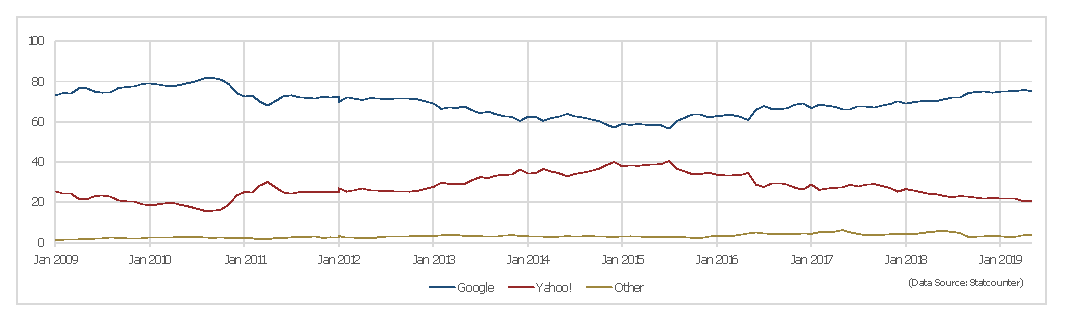
\includegraphics[width=0.95\textwidth,trim=4 4 4 4,clip]{images/searchengine.eps}
 \end{figure}

\subsection{Google Trends}\label{google-trends}

\label{appendix:googletrends}

This graph indicates peak interest over a duration of time and contrasts
interest thus on a relative scale; it does not scale Japanese results to
worldwide results quantitatively.

\subsection{\texorpdfstring{\ref{fig:politictrends}}{}}\label{section-1}

\textbf{Figure \ref{fig:politictrends}} suggests a global increase in
public awareness of politics (the frequency of searches in part of the
total amount of searches has practically doubled) and dominated by a
search interest in left-wing topics (crossed by right-wing topics one
only in November 2016, in the wake of the presidential elections). In
Japan however, interest in political topics as measured by Google Trends
remains however fairly stable throughout the line, with one significant
voorbarig

\begin{figure}[!htb]
 \caption{\label{fig:politictrends} The Google Trends of Right-Wing and Left-Wing Politics Worldwide \& Japan (15 Years).}
 \centering 
 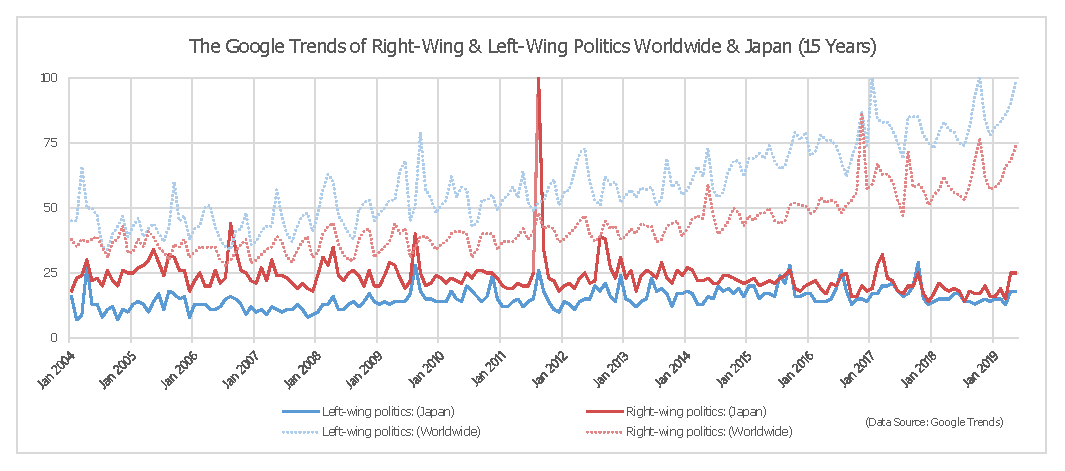
\includegraphics[width=0.95\textwidth,trim=4 4 4 4,clip]{images/politictrends.eps}
\end{figure}

\textbf{Figure \ref{fig:netto-altright}}

\begin{figure}[!htb]
 \caption{\label{fig:netto-altright} Google Trends Breakdown by Region of Netto-Uyoku \& Alt-Right as Topics (15 Years).}
 \centering
 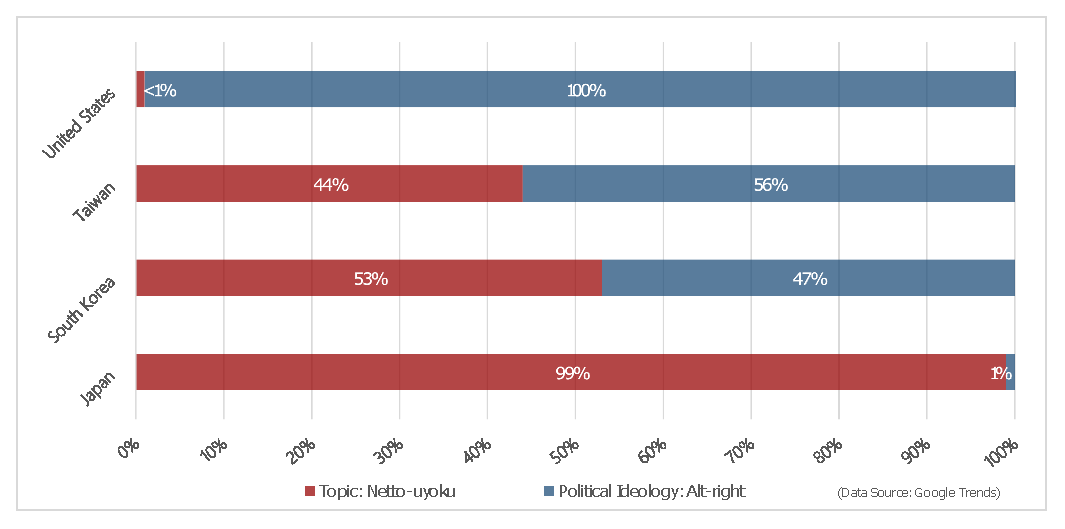
\includegraphics[width=0.95\textwidth,trim=4 4 4 4,clip]{images/netto-altright.eps}
\end{figure}

\textbf{Figure \ref{fig:netto-altright-kor}}

\begin{figure}[!htb]
 \caption{\label{fig:netto-altright-kor} The Google Trends of Netto-Uyoku \& South Korea Since 2010.}
 \centering
 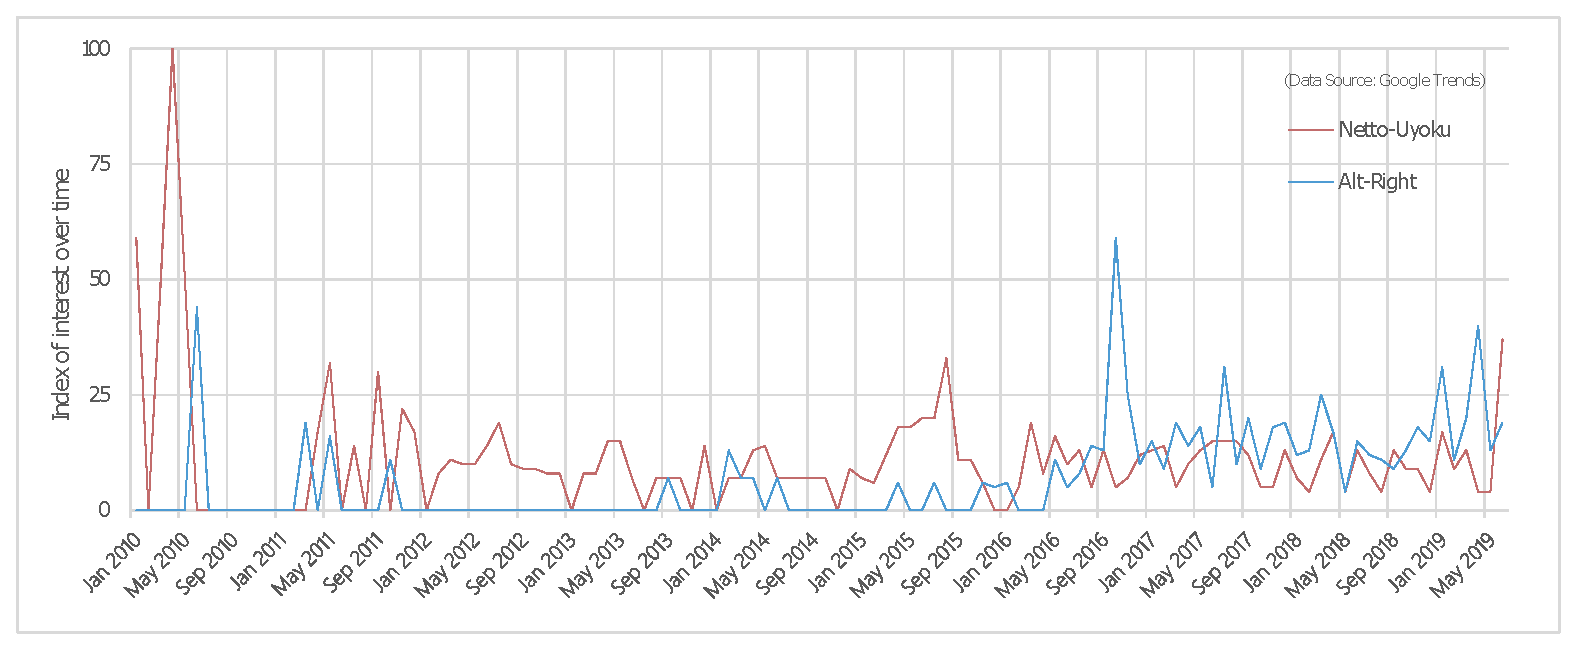
\includegraphics[width=0.95\textwidth,trim=4 4 4 4,clip]{images/netto-altright-kor.eps}
\end{figure}

\section{Other}\label{other}

Edit later

\section{Wikipedia}\label{wikipedia}

\subsection{Wikipedia Reverts}\label{wikipedia-reverts}

In order to calculate contentious Japanese Wikipedia pages I use a
rudimentary way of comparing the total amount of reverts to the total
amount of revisions on a page (limited to articles, I exclude
\emph{namespaces} for pages such as \emph{Userpages}). I wrote a script
in the Java programming language to obtain the top 1000 revised articles
(both in total and during a certain time span). My dataset is a 5GB
data-dump (\emph{jawiki-20190620-stub-meta-history.xml.gz}) obtained
from \url{https://dumps.wikimedia.org/jawiki/20190620/}. This compressed
file contains an XML file with meta-data of every Japanese Wikipedia
page (such as title, namespace, and revision information) up to
2019-06-20.\footnote{For more information on the elements of this XML
  dump, see
  \url{https://glimmerphoenix.github.io/WikiDAT/pages/meta-history/}.}
Reverts are then based on keywords (eg. `rv', `取り消し', `巻き戻し') in
the comments of revisions and are therefore not completely exhaustive
(this would most likely include reverts of acts of vandalism, but will
not include the actual act of vandalism in which one reverts parts of-
or even the complete article). While this methodologically requires
further attention, preliminary results undeniable show in quantifiable
ways particular political topics to be in the top of so-called
`\emph{Wiki edit-wars}'. I ran the script for each year between the
range of 2003 (the beginning of the data-dump) and 2019. Per year I
included levels of controversy based both on the total amount of
revisions and reverts up to that year, as well as solely on the
revisions and reverts committed in that particular frame of time.

\section{Tables}\label{tables}

\subsection{50 Most Popular Websites in Japan
(2019)}\label{most-popular-websites-in-japan-2019}

These statistics are calculated on a three-monthly basis, determined by
a combined page views and unique visitors of all pages belonging to one
particular domain (Alexa - Top Sites in Japan - Alexa
\protect\hyperlink{ref-noauthor_alexa_2019}{2019}).

\begin{table}[!htb]
\footnotesize
\centering
\setlength{\tabcolsep}{5pt}
\caption{50 Most Popular Websites in Japan (2019)}\label{tab:50mostpopjp}
\scalebox{0.8}{
\begin{tabular}{@{}p{0.1cm}lp{0.1cm}lp{0.1cm}lp{0.1cm}lp{0.1cm}lp{0.1cm}lp{0.1cm}lp{0.1cm}l@{}}
\toprule
1&Google.com&11&Fc2.com&21&Amazon.com&31&Blogspot.com&41&Msn.com\\
2&YouTube.com&12&T.co&22&Yahoo.com&32&Tmall.com&42&Nikkei.com\\
3&Yahoo.co.jp&13&Baidu.com&23&Qq.com&33&Apple.com&43&5ch.net\\
4&Amazon.co.jp&14&Instagram.com&24&Mercari.com&34&Microsoft.com&44&Naver.jp\\
5&Google.co.jp&15&Kakaku.com&25&Goo.ne.jp&35&Taobao.com&44&Dmm.com\\
6&Twitter.com&16&Livedoor.jp&26&Blog.jp&36&Netflix.com&46&Nhk.or.jp\\
7&Facebook.com&17&Livedoor.com&27&Weblio.jp&37&Pixiv.net&47&Line.me\\
8&Rakuten.co.jp&18&Ameblo.jp&28&Live.com&38&Japanpost.jp&48&Sohu.com\\
9&Wikipedia.org&19&Dmm.co.jp&29&Hatenablog.com&39&Github.com&49&Office.com\\
10&Nicovideo.jp&20&Pornhub.com&30&Xvideos.com&40&Impress.co.jp&50&Tabelog.com\\
\bottomrule
\end{tabular}
}
\end{table}

\subsection{Japanese Wikipedia Top 50 (as of
2019)}\label{japanese-wikipedia-top-50-as-of-2019}

\label{sec:wikiappendix}

Based on respectively my measurement of controversy (reverts divided by
revisions), the total amount of revisions and the total amount of
reverts, I compiled a list of the 50 highest ranking articles.

\begin{table}
\footnotesize
\centering
\setlength{\tabcolsep}{5pt}
\caption{50 most contentious, revised and reverted articles on the Japanese Wikipedia (2019)}\label{tab:50expanded}
\scalebox{0.9}{
\begin{tabular}{@{}p{0.1cm}lll@{}}
\toprule
&Top 50 contentious articles&Top 50 revised articles&Top 50 reverted articles\\
\midrule
1&南京事件&ZIP!&AKB48\\
2&ネット右翼&海賊戦隊ゴーカイジャー&安倍晋三\\
3&日本&ONE PIECEの登場人物一覧&日本\\
4&前田敦子&天才てれびくんシリーズのドラマ&ONE PIECE\\
5&王下七武海&ゲゲゲの鬼太郎の登場キャラクター&前田敦子\\
6&悪魔の実&WWEに所属する人物一覧&乃木坂46\\
7&ONE PIECE&オールスター感謝祭&創価学会\\
8&渡辺麻友&アニメ+&南京事件\\
9&乃木坂46&めざましテレビ&悪魔の実\\
10&AKB48&名探偵コナンの登場人物&王下七武海\\
11&安倍晋三&ちちんぷいぷい (テレビ番組)&ネット右翼\\
12&欅坂46&相棒の登場人物&けいおん!\\
13&鳩山由紀夫&ONE PIECEの登場人物一覧&ONE PIECEの登場人物一覧\\
14&創価学会&3年B組金八先生)&海賊 (ONE PIECE)\\
15&天皇&SASUKE&渡辺麻友\\
16&中華民国&青森放送&仮面ライダーシリーズ登場怪人一覧\\
17&おそ松さん&海賊 (ONE PIECE)&大韓民国\\
18&金妍兒&AKB48/log20110116&天皇\\
19&在日特権を許さない市民の会&イナズマイレブンの登場人物&嵐 (グループ)\\
20&指原莉乃&情報ライブ ミヤネ屋&海軍 (ONE PIECE)\\
21&在日韓国・朝鮮人&フジテレビジョン&モンキー・D・ルフィ\\
22&櫻井翔&福山潤&在日特権を許さない市民の会\\
23&上皇明仁&SMAP&鳩山由紀夫\\
24&YouTube&グルメチキンレース・ゴチになります!&在日韓国・朝鮮人\\
25&モンキー・D・ルフィ&新日本プロレス&プリキュアシリーズ\\
26&朝日新聞&仮面ライダーフォーゼ&仮面ライダーゴースト\\
27&本田圭佑&ゲームセンターCX&SMAP\\
28&スカパー! チャンネル一覧&めちゃ×2イケてるッ!&SKE48\\
29&ONE PIECEの用語一覧&スーパー戦隊シリーズ&水樹奈々\\
30&仮面ライダーシリーズ登場怪人一覧&AKB48&AKB48\\
31&けいおん!&読売ジャイアンツ&指原莉乃\\
32&艦隊これくしょん -艦これ-&相棒&中華民国\\
33&海軍 (ONE PIECE)&プリキュアシリーズ&福山潤\\
34&高橋みなみ&モーニング娘。&Hey! Say! JUMP\\
35&仮面ライダーゴースト&仮面ライダーディケイド&欅坂46\\
36&松本人志&24時間テレビ 「愛は地球を救う」&ドラえもん\\
37&動物戦隊ジュウオウジャー&成田国際空港&サザエさんの登場人物\\
38&朝鮮民主主義人民共和国&アニメ版ポケットモンスターの登場人物&ONE PIECEの用語一覧\\
39&有吉弘行&仮面ライダー電王&本田圭佑\\
40&HKT48&銀魂 (アニメ)&魔法少女まどか$\star$マギカ\\
41&大韓民国&BLEACHの登場人物&相棒\\
42&手裏剣戦隊ニンニンジャー&関西国際空港&B'z\\
43&初音ミク&安倍晋三&イチロー\\
44&魔法つかいプリキュア!&仮面ライダー鎧武/ガイム&朝鮮民主主義人民共和国\\
45&Fate/Grand Order&阪神タイガース&上皇明仁\\
46&魔法少女まどか$\star$マギカ&トリコ&織田信長\\
47&木村拓哉&龍が如くシリーズの登場人物&二宮和也\\
48&NARUTO -ナルト-の登場人物&ジャニーズJr.&ドラゴンボール\\
49&Minecraft&スーパーJチャンネル&櫻井翔\\
50&韓国起源説&SKE48&FAIRY TAILの登場人物\\
\bottomrule
\end{tabular}
}
\end{table}

\subsection{Methodology)}\label{methodology}

\label{sec:methodology}


\end{document}
